% ---- Document Class ----
\documentclass[sn-mathphys,Numbered]{sn-jnl}


% ---- Essential Packages ----
% FIX: Load xcolor ONCE with all necessary options to prevent "Option Clash"
\usepackage[table,dvipsnames,svgnames]{xcolor}
\usepackage{amsmath}
% FIX: Handle \Bbbk conflict before loading amssymb
\let\Bbbk\relax 
\usepackage{amssymb}
\usepackage{mathtools}
\usepackage{amsthm}
\usepackage{graphicx} % FIXED: Removed [demo] option
%\usepackage{hyperref}

% ---- Formatting & Layout ----
\usepackage{alltt}
\usepackage{paralist}
\usepackage{booktabs}
\usepackage{multirow}
\usepackage{arydshln}
%\usepackage{wrapfig}
\usepackage{hyperref}
\usepackage[capitalize]{cleveref}
\usepackage[export]{adjustbox}
\usepackage{enumitem}
\usepackage{float}
%\usepackage{caption}
%\usepackage{subcaption}
\usepackage{tcolorbox}
\usepackage{nicefrac}
\usepackage{subcaption}
% ---- Code Listings ----
\usepackage{listings}
\usepackage{verbatim}

% ---- Math & Symbols ----
\usepackage{mathpartir}
\usepackage{wasysym}
\usepackage{pifont}
\usepackage{stmaryrd}
\usepackage{bussproofs}
\usepackage{gensymb}
\usepackage[per-mode=symbol,detect-all]{siunitx}
\usepackage{makecell} % in preamble

% ---- Other Utilities ----
\usepackage{xspace}
\usepackage{url}
% FIXED: Removed svg package (requires Inkscape/external tools)
% \usepackage{svg}
\usepackage{ifthen}
\usepackage{etoolbox}
\usepackage[outline]{contour}

% ---- TikZ Graphics ----
\usepackage{tikz}
\usetikzlibrary{shapes.geometric,positioning,arrows}

% ---- Cleveref (Must be loaded after hyperref) ----
\usepackage[capitalize]{cleveref}

% ---- Custom Definitions & Macros ----
% Theorem environments
\newtheorem{theorem}{Theorem}[section]
\newtheorem{lemma}[theorem]{Lemma}
\newtheorem{proposition}[theorem]{Proposition}
\newtheorem{corollary}[theorem]{Corollary}
\theoremstyle{definition}
\newtheorem{definition}[theorem]{Definition}
\theoremstyle{remark}
\newtheorem{remark}[theorem]{Remark}

% Colors
\definecolor{brightyellow}{RGB}{255,247,192}
\definecolor{lightchacki}{RGB}{245,237,205}
\definecolor{darkorange}{RGB}{255,140,0}
\definecolor{headerbg}{RGB}{220,230,241}

% Symbols
\newcommand{\cmark}{\checkmark}
\newcommand{\xmark}{\textcolor{red}{\ding{55}}}
\newcommand{\greencmark}{\textcolor{green}{\ding{51}}}

% Math Macros
\newcommand{\cfg}[3]{\langle #1,\; #2,\; #3\rangle}
\newcommand{\update}[3]{#1[#2 \mapsto #3]}
\newcommand{\step}{\mathrel{\rightarrow}}
\newcommand{\pstep}{\mathrel{\Rightarrow}}
\newcommand{\Pre}{\mathsf{pre}}
\newcommand{\Post}{\mathsf{post}}
\newcommand{\toolname}{\textsc{Ser}}
\newcommand{\grammartag}[1]{\qquad\qquad\emph{(#1)}}

% Keywords
\newcommand{\kw}[1]{\textbf{#1}}
\newcommand{\nondet}{\kw{?}}
\newcommand{\ifkw}{\kw{if}}
\newcommand{\elsekw}{\kw{else}}
\newcommand{\whilekw}{\kw{while}}
\newcommand{\yieldkw}{\kw{yield}}
\newcommand{\requestkw}{\kw{request}}
\newcommand{\sat}{\texttt{SAT}}
\newcommand{\unsat}{\texttt{UNSAT}}
\newcommand{\Parikh}{\mathsf{Parikh}}

% Helper commands
\newcommand\blfootnote[1]{%
	\begingroup
	\renewcommand\thefootnote{}\footnote{#1}%
	\addtocounter{footnote}{-1}%
	\endgroup
}
\newcommand{\guy}[1]{\marginpar{\textcolor{orange}{Guy: #1}}}
\newcommand{\jules}[1]{\marginpar{\textcolor{red}{Jules: #1}}}
\newcommand{\markb}[1]{\marginpar{\textcolor{black}{Mark: #1}}}
\newcommand{\todo}[1]{\textcolor{red}{TODO: #1}}

% Listings Configuration
\lstdefinelanguage{CustomPseudoCode}{
	morekeywords={request, yield, return, if, else, while, and, or},
	morecomment=[l]{//},
	morestring=[b]",
	sensitive=true
}
\lstset{
	language=CustomPseudoCode,
	basicstyle=\ttfamily\small,
	keywordstyle=\color{blue}\bfseries,
	commentstyle=\color{gray}\itshape,
	stringstyle=\color{orange},
	numbers=left,
	numberstyle=\tiny,
	stepnumber=1,
	numbersep=5pt,
	backgroundcolor=\color{white},
	frame=single,
	rulecolor=\color{black},
	tabsize=2,
	captionpos=b,
	breaklines=true,
	breakatwhitespace=false,
	showstringspaces=false,
	escapeinside={(*@}{@*)},
}

% Hyperref fixes
%\makeatletter
%\renewcommand*{\theHsection}{\thesection}
%\renewcommand*{\theHsubsection}{\thesubsection}
%\renewcommand*{\theHsubsubsection}{\thesubsubsection}
%\patchcmd{\@sect}
%{\@tempskipa #5\relax}
%{\refstepcounter{#1}%
%	\Hy@raisedlink{\hyper@anchorstart{#1.\csname the#1\endcsname}\hyper@anchorend}%
%	\@tempskipa #5\relax}
%{}{}
%\makeatother

\let\Bbbk\relax


% ==========================================
%            DOCUMENT START
% ==========================================
\begin{document}
	
	\title{Verifying Unbounded Serializability in\\ Network Systems}
	
	\author*[1]{\fnm{Guy}\sur{Amir}}\email{gda42@cornell.edu}
	\author[1]{\fnm{Mark}\sur{Barbone}}\email{mlb494@cornell.edu}
	\author[2]{\fnm{Nicolas}\sur{Amat}}\email{nicolas.amat@onera.fr}
	\author[1,3]{\fnm{Jules}\sur{Jacobs}}\email{jj758@cornell.edu}
	
	\affil[1]{\orgname{Cornell University}, \orgaddress{\city{Ithaca}, \country{United States}}}
	
	\affil[2]{\orgname{DTIS, ONERA, Universit\'e de Toulouse}, \orgaddress{\city{Toulouse}, \country{France}}}
	
	\affil[3]{\orgname{Jane Street Capital}, \orgaddress{\city{New York City}, \country{United States}}}
	
	\abstract{
		We present the \toolname{} toolchain and modeling language for automatically verifying \textit{serializability} of concurrent programs, i.e., whether every concurrent execution of the program is equivalent to some serial execution.
		%
		\toolname{} programs are deliberately restricted in order to make this problem decidable, while allowing an unbounded number of concurrent threads, each potentially running for an unbounded number of steps.
		%
		Prior work has shown the theoretical decidability of this problem, but \toolname{} is the first to provide an end-to-end decision procedure and toolchain that proves serializability (generating a certificate) or non-serializability (generating a counterexample trace).
		%
		Our verifier translates network system programs into Petri nets, and curtails the search space by employing various optimizations, such as Petri net slicing, semilinear-set compression, and Presburger-formula manipulation.
		%
		We extensively evaluate our toolchain and demonstrate that, despite the theoretical hardness of the problem, it can successfully run on various models of real-world programs, including BGP routers, stateful firewalls,  online shopping backends, and more.
	}
	
	\keywords{Serializability, Concurrent programs, Network systems, Petri nets, Decision procedure}
	
	\maketitle
%	\pagestyle{plain}
%	\thispagestyle{plain}
	


	 \section{Introduction}
\label{sec:introduction}

\todo{Introduction goes here.}

\todo{We motivate the problem of deciding serializability in programmable networks.}

\todo{We talk about some related work if relevant.}

\todo{We show that it's interesting with an example.}

\todo{We describe our main results.}

\paragraph{Contributions:}
\begin{itemize}
    \item Novel notion of serializability (``atomicity'') applicable to network systems
    \item Decidability results (1 main theorem: \textbf{automatically proving unbounded serializability}, 2 extra theorems: ser=ser decidable, ser=int undecidable)
    \item Implementation of decision procedure
    \item Advances in semilinear sets, Petri net reachability heuristics that makes the decision procedure work
\end{itemize}
	 %\newpage


\section{Tour / examples}
\label{sec:tour}

Next, we will walk through a series of examples, in varying level of complexity. Each example will demonstrate different aspects of serializable vs non-serializable programs.
%
The first examples are relatively basic, while the last examples have higher complexity and are motivated by real word problems, e.g., BGP routing policy updates.
%
Global variables are depicted with upper-case characters, while local variables (per each request) are depicted with lower-case ones.
%
Unless explicitly state otherwise, all global and local variables are initialized to 0.
%
The ``\textit{?}'' symbol depicts a nondeterministic choice between ``0'' and ``1''. All other constructs (\textit{while}, \textit{yield} \textit{if}) have their common interpretation.

\guy{Is the above paragraph clear?}

\subsection{Example 1}

%\subsubsection{Example 1}

We start with a basic example, describing a single request {\color{ForestGreen}$\blacklozenge_\text{A}$}, a single local variable (``x'') per each request; and a single global variable (``FLAG'') shared among all in-flight requests. 
%
In Listing~\ref{lst:BasicSer} an in-flight request assigns to x the value of FLAG (hence, initially, [$x:=0$]). Then, the request non-deterministically chooses whether to yield, or to flip the value of $x$. Subsequently, FLAG is assigned 1 and the value of x is returned as the response to request {\color{ForestGreen}$\blacklozenge_\text{A}$}. 
%
Note that the presence of the \textit{else} branch renders the program serializable, as intuitively, the returned value of x does not depend on the assignment of FLAG.
%
However, this changes in  Listing~\ref{lst:BasicNonSer}. In which case there is no ``else'' branch and x is always assigned the value of FLAG.
%
It is straightforward to see that this update makes the program non-serializable. Any serial execution will afford the first request {\color{ForestGreen}$\blacklozenge_\text{A}$} the matching returned response {\color{red}$\blacklozenge_0$} (as $[x:=FLAG]$, which is initially 0). As the first request also assigns $[FLAG:=1]$ before exiting, any subsequent execution will assign $[x:=1]$ and hence return the response {\color{red}$\blacklozenge_1$}. Differently put, for any serial execution with i requests --- we have exactly one (first) request/response pair {\color{ForestGreen}$\blacklozenge_\text{A}$}/{\color{red}$\blacklozenge_0$}, and $(i-1)$ pairs of {\color{ForestGreen}$\blacklozenge_\text{A}$}/{\color{red}$\blacklozenge_1$}.
%
However, given that the first request can also \textit{yield}, it is possible for another request to subsequently run the program after the first request yields and before it returns. This, in turn, will allow two requests to have $[x=0]$, and hence, any number of arbitrary requests can have multiple {\color{ForestGreen}$\blacklozenge_\text{A}$}/{\color{red}$\blacklozenge_0$} pairs. Thus, Listing~\ref{lst:BasicNonSer} is not serializable.




%\vspace{2em}
%example - 2

% Second row
\noindent
\begin{minipage}[t]{0.45\textwidth}
	\begin{lstlisting}[caption={Serializable},
		label={lst:BasicSer}]
	request A: 
		x := FLAG
		
		if (?):
			yield
		else:
			x := 1 - x
		
		FLAG := 1
		return x
	\end{lstlisting}
\end{minipage}
\hfill
\begin{minipage}[t]{0.45\textwidth}
	\begin{lstlisting}[caption={Not serializable: {(A,0),(A,0)}},
	label={lst:BasicNonSer}]
			request A: 
			    x := FLAG 
			
			    if (?): 
			        yield
			    // no else
			
			
			    FLAG := 1 
			    return x
		\end{lstlisting}
\end{minipage}%

\subsection{Example 2}

%\subsubsection{Example 2}
The following program pairs have a single global variable ``X'', and two requests --- {\color{ForestGreen}$\blacklozenge_\text{incr}$} which increments X by 1, and {\color{ForestGreen}$\blacklozenge_\text{decr}$} which decrements X by 1. Both program have while loops which guarantee that X will always be assigned a value between 0 to 3, otherwise the while loop will yield an infinitum. Both requests return the value of X after updating it.
%
In the first case, Listing~\ref{lst:FredSer} presents a serializable execution, due to the absence of any yield between the increment/decrement of X, and its return. Equivalently, in each of the requests, the update of X and the returned value can be thought of as \textit{a single atomic execution}.
%
However, in Listing~\ref{lst:FredNonSer},we add an additional yield (and a local variable ``y''), occurring in each of the requests, between the update of X and it's return.
%
This updates allows request of the same type to update X to the same value --- something that is not possible in any serial execution. 

%\vspace{2em}
%\newpage
%example - 3

% Third row
\noindent
\begin{minipage}[t]{0.45\textwidth}
	\begin{lstlisting}[caption={Fred (serializable)},
		label={lst:FredSer}]
			request incr: 
			    while (X == 3):
			        yield
			        
			        
			    X := X + 1
				  return X		
			
			request decr: 
			    while (X == 0): 
			        yield
			        
			        
			    X := X - 1
				  return X
		\end{lstlisting}
\end{minipage}
\hfill
\begin{minipage}[t]{0.45\textwidth}
	\begin{lstlisting}[caption={Fred2 (not serializable)},
		label={lst:FredNonSer}]
			request incr:
			    while (X == 3):
			        yield
			    y := X
			    yield
			    X := y + 1
		      return X		
			
			request decr: 
			    while (X == 0):
			        yield
			    y := X
			    yield
			    X := y - 1
		      return X
		\end{lstlisting}
\end{minipage}
	
\subsection{Example 3}
%\subsubsection{Example 3}	
%\todo{continue}	
%example - 6

The next pair of examples cover a setting in which there is a single global variable (X) and a single local variable per each in-flight request. The {\color{ForestGreen}$\blacklozenge_\text{flip}$} requests flips the bit of the single initial variable X (initialized to 0); the {\color{ForestGreen}$\blacklozenge_\text{main}$} request attempts to decrement i five times.
%
It is straightforward to observe that the program in Listing~\ref{lst:ComplexWhileSer} is trivially serializable, as there are no yields.
%
However, by adding the two yields and updating the program (see Listing~\ref{lst:ComplexWhileNonSer}) it becomes non-serializable. This can be observed as follows --- given a single in-flight request, the value of X is either 0 or 1, and hence, exactly one of the while loops will run indefinitely. Thus, any serializable execution will result into a set without any {\color{ForestGreen}$\blacklozenge_\text{main}$}/{\color{red}$\blacklozenge_1$} pairs, but rather only, perhaps terminating {\color{ForestGreen}$\blacklozenge_\text{flip}$} requests.
%
However, given at least $i=5$ interleaving of in-flight {\color{ForestGreen}$\blacklozenge_\text{flip}$} requests, it is possible for a {\color{ForestGreen}$\blacklozenge_\text{main}$} request to terminate and bypass all while loops, something that cannot occur in serializable executions.


% Second row
\noindent
\begin{minipage}[t]{0.45\textwidth}
	\begin{lstlisting}[caption={Complex while (serializable)},
		label={lst:ComplexWhileSer}]
		    request flip: 
		        X := 1 - X 
		    
		    request main:
		        i := 5
		        while (i > 0):
		            while (X == 0):
		                pass
		            while (X == 1):
		                pass
		            i := i - 1
		        
		        return 1       
				\end{lstlisting}
\end{minipage}%
\hfill
\begin{minipage}[t]{0.45\textwidth}
	\begin{lstlisting}[caption={Complex while with yields (not serializable)},
		label={lst:ComplexWhileNonSer}]
		    request flip: 
		        X := 1 - X 
		
		    request main:
		        i := 5
		        while (i > 0):
		            while (X == 0):
		                yield
		            while (X == 1):
		                yield
		            i := i - 1
		
		        return 1        
					\end{lstlisting}
\end{minipage}
	
	
	
\subsection{Example 4}
%\subsubsection{Example 4: Banking System}

The next example emulates a simple banking system, as motivated by Chandy and Lamport's seminal paper~\cite{ChLa85}. The system operates on two accounts of the same user --- denoted with the global variables $A$ and $B$, and initialized to have $100\$$ and $50\$$ respectively. 
%
Each {\color{ForestGreen}$\blacklozenge_\text{transfer}$} request allocates $50\$$ from account $A$ to account $B$, and every {\color{ForestGreen}$\blacklozenge_\text{interest}$} request adds $t\%$ interest to each account. For simplicity, and without loss of generality, we chose $t=100\%$, hence doubling the funds in each account, per each such request. We also note that for simplicity we depict two accounts ($A$ and $B$), although this example is valid for any number of accounts.
%
Both requests return the sum of final client funds in both the accounts.  
%
Listing~\ref{lst:BankSer} depicts a serializable version of this banking system (without any yields), while Listing~\ref{lst:BankNonSer} includes yields in each of the requests, between the adjustment of accounts $A$ and $B$ (we note that this also represents real world systems in which the account can be sharded and partitioned across different nodes).
%


\noindent
\begin{minipage}[t]{0.45\textwidth}
	\begin{lstlisting}[caption={bank (serializable)},
		label={lst:BankSer}]
	    // initialize accounts
	    A := 100
	    B := 50
	    
	    request transfer: 
	        // transfer 50$
	        A := A - 50
	        // no yield
	        B := B + 50
	        return A + B
				
	    request interest: 
	        // add a 100% interest
	        A := A + A
	        // no yield
	        B := B + B
	        return A + B	      		        
			\end{lstlisting}
\end{minipage}
\hfill
\begin{minipage}[t]{0.45\textwidth}
	\begin{lstlisting}[caption={bank with yields (non serializable)},
		label={lst:BankNonSer}]
	    // initialize accounts
	    A := 100
	    B := 50
			
	    request transfer: 
	        // transfer 50$
	        A := A - 50
	        yield
	        B := B + 50
	        return A + B
	
	    request interest: 
	        // add a 100% interest
	        A := A + A
	        yield
	        B := B + B
	        return A + B	      		        
		\end{lstlisting}
\end{minipage}
	

Interestingly, in this setting, serializability also corresponds to correctness invariants pertaining to the program. Specifically, in every serializable execution, it holds that for $A_{\textit{before}},B_{\textit{before}}$ marking the funds before running a single {\color{ForestGreen}$\blacklozenge_\text{interest}$} request, and any number of {\color{ForestGreen}$\blacklozenge_\text{transfer}$} requests (and $A_{\textit{after}},B_{\textit{after}}$ marking the corresponding state after those requests), then:
\[
\bigl(A_{\mathit{after}} + B_{\mathit{after}}\bigr)
= (1 + t\%)\,\bigl(A_{\mathit{before}} + B_{\mathit{before}}\bigr).
\]

This invariant always holds for any such serial execution, while having the specific division \textit{between} accounts $A$ and $B$ depending on the actual order of the serial execution.
%
However, this correctness invariant does not hold for non serializable executions. For example, in a setting in which there is a single {\color{ForestGreen}$\blacklozenge_\text{transfer}$} request, which deduces $50\%$ from account $A$, and then yields (resulting to a temporary state in which $[A=50\$,B=50\$]$); subsequently followed by an  {\color{ForestGreen}$\blacklozenge_\text{interest}$} request which runs until completion, in which case  $[A=100\$,B=100\$]$, and then, the remainder of the yielded {\color{ForestGreen}$\blacklozenge_\text{transfer}$} request is executed, resulting finally to $[A=100\$, B=150\$]$.  This result in $50\$$ ``missing'' from our system, due to this non serializable behavior.
%
As mentioned, a serial execution of a these two request will always result to 
$A+B=2\cdot (100\$+50\$)=300\$$, with either a final state of $[A=150\$, B=150\$]$ or $[A=100\$, B=200\$]$, depending on the scheduled serializable order.




%\newpage
\subsection{Example 5}

The following example motivates our routing‐policy programs in software‐defined networking (SDN). In SDN, switches not only forward packets but can also be programmed in domain‐specific languages (e.g., P4). At runtime, a centralized controller node can adjust the global network control policy. The controller can also periodically send control packets to each switch, causing it to adopt its updated routing as dictated by the updates.
%
An instance of a simple network with two competing policies is shown in Fig.~\ref{fig:BgpRoutingPolicies}. This network consists of four nodes (numbered 0 through 3), with the two middle nodes --- node 1 (labeled \textit{WEST}) and node 2 (labeled \textit{EAST}), serving as ingress points from where traffic may nondeterministically enter the network. The controller selects one of two policies: a \textcolor{NavyBlue}{blue} policy, which routes traffic from West to East, or a \textcolor{darkorange}{orange} policy, which routes it in the opposite direction.


%// [WEST, switch 1] ---> [EAST, switch 2] ---> [out, switch 3] 
%else:
%B := 0 // red/orange policy
%// [out, switch 0] <--- [WEST, switch 1] <--- [EAST, switch 2] 

\begin{wrapfigure}{r}{0.45\textwidth}  % “r” = wrap on the right, width = 45% of line
	\centering
	\includegraphics[
	width=\linewidth,
	trim=10 15 15 5,   % {left bottom right top} — tweak as needed
	clip
	]{plots/east_west_routing_updated_colors.pdf}
	\caption{Routing policy in example 5.}
	\label{fig:BgpRoutingPolicies}
\end{wrapfigure}

%\begin{figure}[H]
%	\centering
%	\includegraphics[width=0.5\linewidth]{plots/east_west_routing_updated_colors.pdf}
%	\caption{Routing policy in example 5.}
%	\label{fig:BgpRoutingPolicies}
%\end{figure}

This SDN-controlled routing policy is realized in the pseudo code in Listing~\ref{lst:BgpNonSerializable}.
%
The program includes a single global variable $B$, indicating if the current routing policy is the  \textcolor{NavyBlue}{blue} policy ($[B=1]$) or the \textcolor{darkorange}{orange} policy ($[B=0]$).
%
The program has three types of requests:
%\begin{itemize}
%	
%	\item
	(i)
	{\color{ForestGreen}$\blacklozenge_\text{policy update}$}:
%	\textit{policy update}:
 represents a controller  update, which nondeterministically decides whether to update the policy (i.e., flip the value of  variable $G$) or not;
%	
%		\item
(ii)
	{\color{ForestGreen}$\blacklozenge_\text{route\_from\_west}$}:
	 this request represents a packet entering the network from the \textit{WEST} node (node 1); and 
%	
%		\item
(iii)
{\color{ForestGreen}$\blacklozenge_\text{route\_from\_east}$}: this request represents a packet entering the network from the \textit{EAST} node (node 2).
	
%\end{itemize}

Each of the routing requests represents a single packet entering the network. The request includes a local \textit{current} variable representing the index of the current node visited. This variable is initialized as the ingress node value, and updated to emulate the chosen routing path. There is also a \textit{visited\_east} variable (or a \textit{visited\_west} variable, depending on the request in question).
%
The return value of the {\color{ForestGreen}$\blacklozenge_\text{route\_from\_west}$} requests is the sum \textit{(current+current+visited\_east)}. This is an identifier encoding all possible \textit{(current\_switch, visited\_east)} pairs.
%
The program is not serializable, as witnessed by an interleaving that can give rise to final return value of \textit{(current+current+visited\_east)=1} (due to \textit{current=0} and \textit{visited\_east=1}). This represents a routing cycle in the network, which is possible only when updated the routing policy after a request has already been routed based on the previous policy.
Legal, acyclic routes of this request have either a return value of 0 (in the case of [\textit{current=0}, \textit{visited\_east=0}]) or 7 (in the case of [\textit{current=3}, \textit{visited\_east=1}]).
Potential routing cycles can also be observed via non serializable executions also for the  {\color{ForestGreen}$\blacklozenge_\text{route\_from\_east}$} requests.



\begin{minipage}[t]{1.0\textwidth}
	\begin{lstlisting}[caption={BGP (non serializable --- cycles can appear)},label={lst:BgpNonSerializable}]
	    // initialize accounts
	    B := 0
	    
	    request policy_update:
	    if (?):
	        B := 1  // blue policy 
	    else:
	        B := 0 // orange policy
			
	    request route_from_west:
	        visited_east := 0
	        current := 1
	        while (current == 2) or (current == 3): // still routing        
	            if (current == 1): // west (switch 1)
	                if (B == 1): // blue policy
	                    current := 2
	                else: // orange policy
	                    current := 1
	            if (current == 2): // east (switch 2)
	                visited_east := 1
	                if (B == 1): // blue policy
	                    current := 3
	                else: // orange policy
	                    current := 1
	 
	            yield
			
	        return current + current + visited_east
	        
	    request route_from_east:
	        ... // dual case     		        
		\end{lstlisting}
\end{minipage}






\subsection{Example 6}

We add an additional example for network monitoring and \textit{snapshot isolation} in Appendix~\ref{}.
%\guy{suddenly I'm not so sure about this example. It is indeed sound but maybe a bit silly?}


The next program is motivated by system monitoring.
The system has two nodes (represented by the global variables $N_1$ and $N_2$) which monitor ongoing traffic in the network, and are originally both active (as indicated by their initial values [$N_1=1,N_2=1$]).
%
The {\color{ForestGreen}$\blacklozenge_\text{main}$} request takes a ``snapshot'' of the system, i.e., locally records the current activation status of each of the two nodes.
%
Subsequently, in the first request, and any future ones in which both nodes are active, each in-flight request thread  non-deterministically decides which of the two nodes to deactivate, i.e. set [$N_i:=0$]. This policy is consistent with real-world settings for maintaining overall energy efficiency.
%
The {\color{ForestGreen}$\blacklozenge_\text{main}$} request eventually returns the current sum of active nodes in the system.
%
In order for the system to emulate multiple iterations, our setting also includes two additional requests, {\color{ForestGreen}$\blacklozenge_\text{activate\_n1}$},{\color{ForestGreen}$\blacklozenge_\text{activate\_n2}$} which activate the nodes $N_1$ and $N_2$, respectively.
%
We note that the program is non-serializable due to the yield operation that appears immediately after the recording (snapshot) of the node activity. One such example for a non-serializable behavior occurs when two {\color{ForestGreen}$\blacklozenge_\text{main}$} requests record two active monitor nodes and yield; Then, having each request turn off the complement node. As a result of each request operating based on its isolated ``snapshot'' of the initial global state, both monitor nodes can be turned off and we can attain a request with {\color{ForestGreen}$\blacklozenge_\text{main}$}/{\color{red}$\blacklozenge_0$} (for [$N_1+N_2=0+0=0$]).
%
We note that in any serializable execution, no two {\color{ForestGreen}$\blacklozenge_\text{main}$} requests can record both monitors as active, and hence, they cannot both have an interleaving in which each separate monitor is deactivated (hence, a response of {\color{red}$\blacklozenge_0$} is unattainable in serializable executions).




\begin{minipage}[t]{1.0\textwidth}
	\begin{lstlisting}[caption={Snapshot-based monitor deactivation (not serializable, as it can return a sum of 0 active monitors)}]
			// initialize both monitors to be active
			N_1_ACTIVE := 1
			N_2_ACTIVE := 1
			
			request main:
				// take snapshot
				n_1_active_snapshot := N_1_ACTIVE
				n_2_active_snapshot := N_2_ACTIVE
				yield
				
				if (n_1_active_snapshot == 1) and (n_2_active_snapshot == 1):
				// if both nodes active --- choose which one to deactivate 
					if (?): 
						  N_1_ACTIVE := 0
					else:
						  N_2_ACTIVE := 0
					
				return N_1_ACTIVE + N_2_ACTIVE  // total active nodes
				
			
			request activate_n1:
				    N_1_ACTIVE := 1
			
			request activate_n2:
				    N_2_ACTIVE := 1
			
			
		\end{lstlisting}
\end{minipage}

%only 0 in non-serializable runs!

%\todo{start}

%/snapshot_isolation_directly_as_NS_with_yields

%\begin{figure}[h]
%	\centering
%	\includegraphics[width=1.0\linewidth]{plots/snapshot\_isolation\_JSON\_with\_yields.pdf}
%	\caption{Snapshot Isolation with Yields.}
%	\label{fig:snapshotIsolationJsonWithYields}
%\end{figure}
%
%
%
%%/snapshot_isolation_directly_as_NS_without_yields
%
%\begin{figure}[h]
%	\centering
%	\includegraphics[width=1.0\linewidth]{plots/snapshot\_isolation\_JSON\_without\_yields.pdf}
%	\caption{Snapshot Isolation without Yields.}
%	\label{fig:snapshotIsolationJsonWithoutYields}
%\end{figure}


%\todo{maybe we have: (1) a copy of the global automaton; (2) a copy of the local automaton (with yields) with coloring of edges that don't exist in the one without yields}


%\begin{figure}[h]
%	\centering
%	\includegraphics[width=0.65\linewidth]{plots/BgpColoredRouting.pdf}
%	\caption{Routing policy in example 7.}
%	\label{fig:pdfimage}
%\end{figure}

%\newpage
%
%
%example – 8
%
%\noindent
%\begin{minipage}[t]{0.45\textwidth}
%	\begin{lstlisting}[caption={foo (serializable)}]
%	request foo: 
%	    if (?):
%	        X := (X + 2) % 3 
%	        // no yield
%	        return X
%	
%	    else:
%	        X := (X + 1) % 3
%	        // no yield
%	        return X
%		\end{lstlisting}
%\end{minipage}
%\hfill
%\begin{minipage}[t]{0.45\textwidth}
%\begin{lstlisting}[caption={foo (non serializable)}]
%request foo: 
%     if (?):
%         X := (X + 2) % 3 
%         yield
%         return X
%
%     else:
%         X := (X + 1) % 3
%         yield
%         return X
%	\end{lstlisting}
%\end{minipage}
%
%One output that is attainable only via non-serializable executions is 
%\[
%\{(foo,1),(foo,1),(foo,1),(foo,3)\}
%\]
%
%
%%\newpage
%
%
%example – 9
%
%\noindent
%\begin{minipage}[t]{0.45\textwidth}
%	\begin{lstlisting}[caption={foo (serializable)}]
%request foo:
%    if(STOP == 0):
%        X := (X + 1) % 4
%
%    yield
%
%    if(STOP == 0):
%        X := (X + 1) % 4
%
%        STOP := ?
%        
%        if(STOP == 1):
%	        return X
%        return 0
%	\end{lstlisting}
%\end{minipage}
%\hfill
%\begin{minipage}[t]{0.45\textwidth}
%	\begin{lstlisting}[caption={foo (non serializable)}]
%request foo:
%    if(STOP == 0):
%        X := (X + 1) % 4
%
%    yield
%
%    if(STOP == 0):
%        X := (X + 2) % 4
%
%        STOP := ?
%        
%        if(STOP == 1):
%	        return X
%        return 0
%	\end{lstlisting}
%\end{minipage}



	 %\newpage
%\vspace{-3.0pt}
\section{Background}
\label{sec:background}
%\guy{Can someone check Sections 3-4-5? Especially the formulations}


%\subsection{Background}
%\label{subsec:background}

%\textbf{Petri nets.} 
\subsection{Petri Nets}
A Petri net $N$ is defined as a five-tuple $N=(P,T,\mathsf{pre},\mathsf{post},M_0)$ with $P$ being a set of places, $T$ being a set of transitions, $\mathsf{pre},\mathsf{post}:T\to\mathbb N^P$ being flow functions, and  $M_0\in\mathbb N^P$ being an initial distribution (a.k.a. \textit{marking}) of tokens in places.  
Transition $t$ is said to be \textit{enabled} at marking $M \in \mathbb N^P$ iff coordinate-wise it holds that $M\ge \mathsf{pre}(t)$, i.e., marking $M$ has at least as many tokens as is required by the flow function $\mathsf{pre}(t)$.
%
A transition \(t\) that is enabled may or may not \textit{fire}. If it fires, it consumes tokens based on $\mathsf{pre}(t)$, and produces tokens based on $\mathsf{post}(t)$. Firing a transition results in a new marking $M'$ (denoted as $M\xrightarrow{t}M'$), and with $M'= M - \mathsf{pre}(t) + \mathsf{post}(t)$. Differently put, firing a transition consumes input tokens and produces output tokens.
%
A single firing can naturally be extended to a firing \textit{sequence} $\sigma = t_1\cdots t_k$ (denoted as $M \xrightarrow{\sigma} M'$), giving rise to a sequence of markings $M_0,\ldots,M_k$ such that $M=M_0$, $M'=M_k$, and for all $i$ it holds that $M_i \xrightarrow{t_{i}} M_{i+1}$. 
% 
We define the (possibly infinite) set $R(N)=\{M \mid \exists \sigma\in T^*. M_0 \xrightarrow{\sigma} M\}$ to include all the markings of the Petri net that are reachable from the initial marking $M_0$.
% 
Given a Petri net $N$ and a marking $M$, the \textit{reachability problem} asks  whether $M\in R(N)$. 
%
Specifically, in this work we focus on reachability of a linear-constraint formula $\mathcal {F}$ over tokens. The formula is \sat\ if there exists a reachable marking $M\in R(N)$ which satisfies the constraints of $\mathcal {F}$ (this is denoted as $M \models \mathcal {F}$); otherwise, the formula is said to be \unsat{}.
%
Surprisingly, the Petri net reachability problem is decidable even in the \textit{unbounded} case, in which the net's places may hold an arbitrary number of tokens~\cite{Ma81,Ko82,La92}. 

\medskip
\noindent
\textbf{Example: PN definition and reachability.} 
%
Observe the toy Petri net in Fig.~\ref{fig:toyPN}.

\begin{figure}[H]
	\centering
	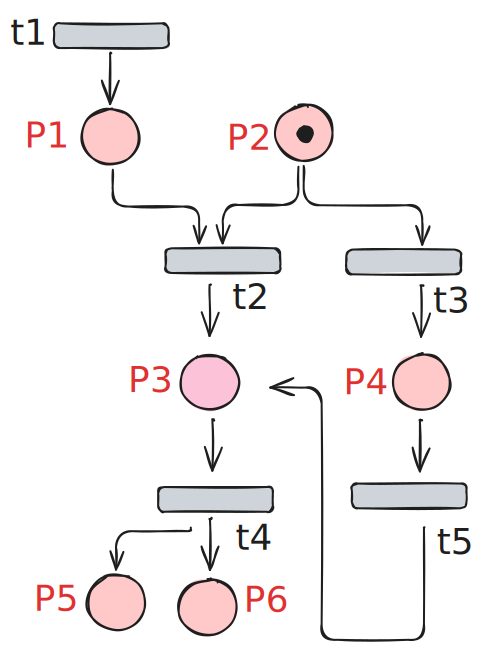
\includegraphics[width=0.3\textwidth]{plots/toy_PN_example.pdf}
	\caption{A toy Petri net.}
	\label{fig:toyPN}
\end{figure}



We formally define the net as follows:
%
\(N=(P,T,\mathsf{pre},\mathsf{post},M_0)\) with
\[
P=\{P_1,P_2,P_3,P_4,P_5,P_6\},\quad
T=\{t_1,t_2,t_3,t_4,t_5\},
\]
and the flow functions $\mathsf{pre}$,$\mathsf{post}$ are given as
\[
\begin{array}{c|cccccc}
	& P_1 & P_2 & P_3 & P_4 & P_5 & P_6 \\ \hline
	\mathsf{pre}(t_1)  & 0 & 0 & 0 & 0 & 0 & 0 \\
	\mathsf{post}(t_1) & 1 & 0 & 0 & 0 & 0 & 0 \\ \hline
	\mathsf{pre}(t_2)  & 1 & 1 & 0 & 0 & 0 & 0 \\
	\mathsf{post}(t_2) & 0 & 0 & 1 & 0 & 0 & 0 \\ \hline
	\mathsf{pre}(t_3)  & 0 & 1 & 0 & 0 & 0 & 0 \\
	\mathsf{post}(t_3) & 0 & 0 & 0 & 1 & 0 & 0 \\ \hline
	\mathsf{pre}(t_4)  & 0 & 0 & 1 & 0 & 0 & 0 \\
	\mathsf{post}(t_4) & 0 & 0 & 0 & 0 & 1 & 1 \\ \hline
	\mathsf{pre}(t_5)  & 0 & 0 & 0 & 1 & 0 & 0 \\
	\mathsf{post}(t_5) & 0 & 0 & 1 & 0 & 0 & 0
\end{array}
\]
The initial marking includes a single token in place $P_2$:
\[
M_0 = (0,1,0,0,0,0)^\top.
\]

%Differently put, there is .


\begin{itemize}
	\item An examples of a \emph{reachable} marking is
	\[
	M_f = (0,0,0,0,1,1)^\top,
	\]
	reached by the firing sequence
	\[
	M_0 \xrightarrow{t_1} M_1
	\xrightarrow{t_2} M_2
	\xrightarrow{t_4} M_f,
	\]
	where
	\[
	M_1 = (1,1,0,0,0,0)^\top,
	\quad
	M_2 = (0,0,1,0,0,0)^\top.
	\]
	\item An example of a \emph{non-reachable} marking is
	\[
	M_{nr} = (0,1,1,0,0,0)^\top.
	\]
	Since producing a token at \(P_3\) (via \(t_2\)) necessarily consumes the only token in \(P_2\) and, as no transition replenishes \(P_2\), it is impossible for these two places to \textit{simultaneously} hold a single token in any reachable firing. However, we note that if the initial marking were 
	
	\[
	M_0' = (0,2,0,0,0,0)^\top,
	\]
	then marking $M_{nr}$ \textit{would have} been reachable, by firing a single transition $t_1$, followed by a single transition $t_2$.
\end{itemize}



%\medskip
%\noindent
%\textbf{Verdict proofs.} 
\subsection{Verdict proofs}
If formula $\mathcal {F}$ is indeed \textit{reachable}, then there exists a witness sequence $\sigma\in T^*$ such that $M_0\xrightarrow{\sigma}M$ and also, $M\models \mathcal {F}$ serves as a proof that can be verified by simulating the Petri net firings.  
However, in the case that formula $\mathcal {F}$ is \textit{unreachable}, then there exists~\cite{Le09} a Presburger certificate $C$ that inductively proves non-reachability: 
(i) $M_0\models C$, (ii) $\forall t\in T \quad (M\models C \wedge M\xrightarrow{t}M')\Rightarrow M'\models C$, and (iii) $C\Rightarrow \neg \mathcal {F}$.

%\medskip
%\noindent
%\textbf{Semilinear sets and Parikh’s theorem.}

\subsection{Semilinear sets and Parikh’s theorem}
A set $S\subseteq\mathbb N^k$ is \textit{semilinear} if and only if it is a finite union of linear sets, i.e., for some $\mathbf b_i,\mathbf p_{i,j}\in\mathbb N^k$ it holds that:
\[S=\bigcup_{i=1}^m \{\mathbf b_i+\sum_{j=1}^{r_i} n_j\mathbf p_{i,j}\mid n_j\in\mathbb N\}.\]
Furthermore, semilinear sets coincide with sets that can be defined by \textit{Presburger arithmetic}~\cite{Pr29}. 
%
In the context of automata theory, Parikh’s theorem~\cite{Parikh66} proves that by applying the \textit{Parikh image} of any context-free language (CFL) --- we can obtain a semilinear set. 
%
The \emph{Parikh image} of a word $w$ over $\Sigma=\{a_1,\dots,a_k\}$ is defined as the vector:
\[
\mathsf{Parikh}(w)\;=\;\bigl(|w|_{a_1},\dots,|w|_{a_k}\bigr)\in\mathbb{N}^k,
\]
with $|w|_{a_i}$ counting occurrences of $a_i$ in $w$.
More generally, for a language $L\subseteq\Sigma^*$:
\[
\mathsf{Parikh}(L)\;=\;\{\mathsf{Parikh}(w)\mid w\in L\}\subseteq\mathbb{N}^k.
\]


%\medskip
%\noindent
%\textbf{Semilinear sets and Parikh’s theorem.} 
%A set $S\subseteq\mathbb N^k$ is \textit{semilinear} iff  
%$S=\bigcup_{i=1}^m \{\mathbf b_i+\sum_{j=1}^{r_i} n_j\mathbf p_{i,j}\mid n_j\in\mathbb N\}$,  
%for $\mathbf b_i,\mathbf p_{i,j}\in\mathbb N^k$.  
%Semilinear sets coincide with sets defined by \textit{Presburger arithmetic}~\cite{Pr29}.  
%By Parikh’s theorem~\cite{Parikh66}, the \textit{Parikh Image} of any context-free language is semilinear, with an effective construction.
%%
%For an alphabet $\Sigma=\{a_1,\dots,a_k\}$ and any word $w\in L\subseteq\Sigma^*$, the $\mathsf{Parikh}$ image is $\mathsf{Parikh}(w)=\{\,a_i^{|w|_{a_i}}\mid a_i\in\Sigma\,\}$, the multiset of symbols appearing in $w$ according to their number of occurrences.


%\med skip
%\noindent
%\textbf{Deciding serializability in unbounded systems.}
\subsection{Deciding serializability in unbounded systems}
Bouajjani et al.~\cite{BoEmEnHa13} have proved that, as a special case of \textit{bounded-barrier linearizability}, serializability in unbounded systems can be reduced to a Petri net reachability problem.


	 %\newpage
%\vspace{-3.0pt}
\section{Problem Definition}
\label{sec:problem-definition}
%\guy{Can someone check Sections 3-4-5? Especially the formulations}


\subsection{The SER Language}

\subsubsection{Syntax}
We define the syntax of our \toolname{} language as follows: 
%of Fig.~\ref{fig:syntax}.

\[
\begin{aligned}
	\mathbf{Expression}\quad e ::= &\ 0 \mid 1 \mid 2 \mid \dots            && \text{numeric constant}\\
	&\mid \nondet                            && \text{nondeterministic\ value (0/1)}\\
%	&\mid x := e
%	&&\text{write to local variable}\\
%	&\mid x
%	&&\text{read from local variable}\\
%	&\mid X := e
%	&&\text{write to global variable}\\
%	&\mid X
%	&&\text{read from global variable}\\
	&\mid x := e \mid x                      && \text{write/read local variable}\\
	&\mid X := e \mid X                      && \text{write/read global variable}\\
	&\mid e_1 == e_2                         && \text{equality test}\\
	&\mid e_1 ; e_2                          && \text{sequencing}\\
	&\mid \ifkw(e_1)\{e_2\}\elsekw\{e_3\}    && \text{conditional}\\
	&\mid \whilekw(e_1)\{e_2\}               && \text{while loop}\\
	&\mid \yieldkw                           && \text{yield to scheduler}
	\\[0.8em]
	\mathbf{Program}\quad P_0 ::= &\ \requestkw\ name_1\{e_1\}\;\dots\;\requestkw\ name_n\{e_n\}
	&& \text{set of handlers} 
\end{aligned}
\]

%
%\[
%\begin{aligned}
%	\mathbf{Expression}\quad e ::={}&{} \\
%	&0 \mid 1 \mid 2 \mid \dots 
%	&&\grammartag{Numeric constants}\\
%	&\nondet
%	&&\grammartag{Nondeterministic value: 0 or 1}\\
%	&x := e
%	&&\grammartag{Write to local variable}\\
%	&x
%	&&\grammartag{Read from local variable}\\
%	&X := e
%	&&\grammartag{Write to global variable}\\
%	&X
%	&&\grammartag{Read from global variable}\\
%	&e_1 == e_2
%	&&\grammartag{Equality test}\\
%	&e_1 ; e_2
%	&&\grammartag{Sequencing}\\
%	&\ifkw(e_1)\{e_2\}\elsekw\{e_3\}
%	&&\grammartag{Conditional}\\
%	&\whilekw(e_1)\{e_2\}
%	&&\grammartag{While loop}\\
%	&\yieldkw
%	&&\grammartag{Yields to scheduler}\\[1em]
%	\mathbf{Program}\quad p ::={}&{} \\
%	&\requestkw\ name_1\{e_1\}
%	&&\grammartag{Set of request handlers}\\
%	&\quad\vdots\\
%	&\requestkw\ name_n\{e_n\}
%\end{aligned}
%\]
%
%%
%
%\begin{figure}[!htbp]
%    \begin{align*}
%    \mathbf{Expression}\quad e ::= &&& \\
%       | & \quad 0 \mid 1 \mid 2 \mid \ldots                                && \grammartag{Numeric constants} \\
%       | & \quad \nondet                                 && \grammartag{Nondeterministic value: 0 or 1}\\
%       | & \quad x := e                            && \grammartag{Write to local variable field} \\
%       | & \quad x                                 && \grammartag{Read from local variable field} \\
%       | & \quad X := e                            && \grammartag{Write to global  variable} \\
%       | & \quad X                                 && \grammartag{Read from global  variable} \\
%       | & \quad e_1 == e_2                        && \grammartag{Equality test} \\
%       | & \quad e_1 ; e_2                         && \grammartag{Sequencing} \\
%       | & \quad \ifkw(e_1)\{\ e_2\ \}\elsekw\{\ e_3\ \} && \grammartag{Conditional} \\
%       | & \quad \whilekw(e_1)\{\ e_2\ \}              && \grammartag{While loop} \\
%       | & \quad \yieldkw                      && \grammartag{Yields to scheduler}\\[1em]
%    \mathbf{Program}\quad p ::=
%        & \quad \requestkw\ name_1\ \{\ e_1\ \}&&\grammartag{Set of request handlers}\\[-0.5em]
%        & \quad \qquad \vdots &&\\
%        & \quad \requestkw\ name_n\ \{\ e_n\ \}\ 
%    \end{align*}
%    \caption{Syntax of expressians and programs}
%    \label{fig:syntax}
%\end{figure}
    %
%    
%
%
%
%\guy{add other rebuttal promises}
%\guy{check semantics}
%
%
% SER small-step semantics with explicit guard (congruence) rules
% Requires: \usepackage{mathtools,amssymb,mathpartir}


%Given such a \(P_0\), we write \(name_i\{e_i\}\in P_0\).
%

Given a program \(P_0\), we write \(name_i\{e_i\}\in P_0\) for each of the handlers \(name_i\{e_i\}\).
%
Our semantics is standard and fully formalized in subsection~\ref{subsec:ser-semantics}. 
 %
 In addition, arithmetic extensions are supported in the tool~\cite{ArtifactRepository} but omitted here for brevity.
%Our semantics is straightforward, and fully formalized in Appendix~\ref{appendix:ser-semantics}.
%
%Furthermore, our syntax and semantics can also be extended with \textit{arithmetic operations} (as implemented in our tool~\cite{ArtifactRepository}), but we omit them for simplicity.
%
%Furthermore, we note that our syntax and semantics can both be extended to include \textit{arithmetic operations} (as in our implementation~\cite{ArtifactRepository}); however, we omit these for simplicity. 
    
\subsubsection{Small-Step Semantics}
\label{subsec:ser-semantics}
%
%
%\subsection{Semantics}
%
The set \(\texttt{V}\) is a finite set of numeric constants; booleans use $0/1$. We respectively denote with \(\texttt{VARS}\) and \(\texttt{vars}\) the (finite) sets of global and local variables. Mappings $\rho:{\texttt{vars}}\to \texttt{V}$ and $g:{\texttt{VARS}}\to \texttt{V}$ respectively map a local or global variable to its current value in \(\texttt{V}\).
%
Configurations are denoted as $\cfg{e}{\rho}{g}$, with \(e\) being a valid \toolname{} expression. 
%
Small steps are denoted $(\step)$, while big steps are denoted $(\pstep)$, and may comprise of a sequence of small steps (denoted $\step^{*}$).
%
%program configurations $\langle g , \Pi\rangle$ with \(g\) being a global state and \(\Pi\) being set of in-flight \((e,\ell)\) pairs.
%
%We denote with \(\ell_0\) the initial local state of every packet.

\smallskip
\noindent\textit{Small step} $(\step)$.
\begin{mathpar}
	\inferrule*[right=ND-0]{ }{\cfg{\nondet}{\rho}{g} \step \cfg{0}{\rho}{g}}
	\and
	\inferrule*[right=ND-1]{ }{\cfg{\nondet}{\rho}{g} \step \cfg{1}{\rho}{g}}\\
	
	\inferrule*[right=LOCAL-READ]{\rho(x)=v\quad v\in{\texttt{V}}}{\cfg{x}{\rho}{g} \step \cfg{v}{\rho}{g}}
	\and
	\inferrule*[right=GLOBAL-READ]{g(X)=v \quad v\in{\texttt{V}}}{\cfg{X}{\rho}{g} \step \cfg{v}{\rho}{g}}\\
	
	\inferrule*[right=LOCAL-WRITE-STEP]{\cfg{e}{\rho}{g} \step \cfg{e'}{\rho'}{g'}}{\cfg{x := e}{\rho}{g} \step \cfg{x := e'}{\rho'}{g'}}
	\and
	\inferrule*[right=LOCAL-WRITE-DONE]{v\in{\texttt{V}}}{\cfg{x := v}{\rho}{g} \step \cfg{v}{\update{\rho}{x}{v}}{g}}
	
	\inferrule*[right=GLOBAL-WRITE-STEP]{\cfg{e}{\rho}{g} \step \cfg{e'}{\rho'}{g'}}{\cfg{X := e}{\rho}{g} \step \cfg{X := e'}{\rho'}{g'}}
	\and
	\inferrule*[right=GLOBAL-WRITE-DONE]{v\in{\texttt{V}}}{\cfg{X := v}{\rho}{g} \step \cfg{v}{\rho}{\update{g}{X}{v}}}
	
	\inferrule*[right=EQ-L]{\cfg{e_1}{\rho}{g} \step \cfg{e_1'}{\rho'}{g'}}{\cfg{e_1 == e_2}{\rho}{g} \step \cfg{e_1' == e_2}{\rho'}{g'}}
	\and
	\inferrule*[right=EQ-R]{\cfg{e_2}{\rho}{g} \step \cfg{e_2'}{\rho'}{g'}}{\cfg{v_1 == e_2}{\rho}{g} \step \cfg{v_1 == e_2'}{\rho'}{g'}}
	\and
	\inferrule*[right=EQ-T]{v_1=v_2\quad v_1, v_2\in{\texttt{V}}}{\cfg{v_1 == v_2}{\rho}{g} \step \cfg{1}{\rho}{g}}
	\and
	\inferrule*[right=EQ-F]{v_1\neq v_2 \quad v_1, v_2\in{\texttt{V}}}{\cfg{v_1 == v_2}{\rho}{g} \step \cfg{0}{\rho}{g}}
\end{mathpar}

\begin{mathpar}
	\inferrule*[right=SEQ-STEP]{\cfg{e_1}{\rho}{g} \step \cfg{e_1'}{\rho'}{g'}}{\cfg{e_1 ; e_2}{\rho}{g} \step \cfg{e_1' ; e_2}{\rho'}{g'}}
	\and
	\inferrule*[right=SEQ-DONE]{v\in{\texttt{V}}}{\cfg{v ; e_2}{\rho}{g} \step \cfg{e_2}{\rho}{g}}
	
	\inferrule*[right=IF-GUARD]{\cfg{e_1}{\rho}{g} \step \cfg{e_1'}{\rho'}{g'}}{\cfg{\ifkw(e_1)\{e_2\}\elsekw\{e_3\}}{\rho}{g} \step \cfg{\ifkw(e_1')\{e_2\}\elsekw\{e_3\}}{\rho'}{g'}}
	\and
	\inferrule*[right=IF-T]{ }{\cfg{\ifkw(1)\{e_2\}\elsekw\{e_3\}}{\rho}{g} \step \cfg{e_2}{\rho}{g}}
	\and
	\inferrule*[right=IF-F]{ }{\cfg{\ifkw(0)\{e_2\}\elsekw\{e_3\}}{\rho}{g} \step \cfg{e_3}{\rho}{g}}
	
	\inferrule*[right=WHILE-UNFOLD]{ }{\cfg{\whilekw(e_1)\{e_2\}}{\rho}{g}
		\step
		\cfg{\ifkw(e_1)\{\,e_2 ; \whilekw(e_1)\{e_2\}\,\}\elsekw\{0\}}{\rho}{g}}
\end{mathpar}

\noindent\textit{Big step} $(\pstep)$ and scheduling.
\begin{mathpar}
	\inferrule*[right=YIELD]{\cfg{e}{\rho}{g} \step^{*} \cfg{\yieldkw ; e'}{\rho'}{g'}}{\cfg{e}{\rho}{g} \pstep \cfg{e'}{\rho'}{g'}}
	\\
	%	\inferrule*[right=START]{\cfg{e_i}{\rho}{g}\pstep \cfg{e'_i}{\rho'}{g'} \quad name_i\{e_i\}\in P_0}{\langle \requestkw\ name_i\{e_i\}, \rho, g \rangle \pstep  \cfg{e'_i}{\rho'}{g'} }
	%	\and
	\inferrule*[right=TERMINATE]{\cfg{e}{\rho}{g} \step^{*} \cfg{v}{\rho'}{g'} \quad v\in{\texttt{V}}}{\cfg{e}{\rho}{g} \pstep \cfg{v}{\rho'}{g'}}	
\end{mathpar}



\smallskip
\noindent
\textbf{Note.}
Instead of defining a \texttt{spawn} instruction, as exists in some languages --- \toolname{} captures \textit{external} spawning via requests.
%
This setting can equivalently capture self-spawning (by using additional global variables), while translating more naturally to the networking domain --- in which threads are captured by packets sent by an external user.


\subsection{Network System}    
Motivated by software-defined networks, we present our abstract network system (NS) abstraction model. Specifically, spawning a new request corresponds to sending a \textit{packet} in the SDN domain --- with each unique \textit{packet header field} representing a request-local \toolname{} variable;
shared variables on \textit{programmable switches}, correspond to global variables, as they are seen by all the requests (packets) visiting the switch. Furthermore, we note that throughout this paper, we use the term \emph{request} to refer to a thread of a concurrent computation unit. 
%
Formally, a network system $\mathcal{N}$ is defined as an eight-tuple $(G, L, \mathit{REQ},  \mathit{RESP}, g_0, \delta, \mathit{req}, \mathit{resp})$ where:
\begin{itemize}
\item $G$ is defined as the set of reachable \textit{global network states} (for example, the values of switch variables)

\item $L$ is defined as the set of reachable \textit{local packet states} (e.g., the values of packet header variables)

\item $\mathit{REQ}$ is a finite set of \textit{request label strings} (with each request label denoted as {\color{ForestGreen}$\blacklozenge_\text{req}$})

\item $\mathit{RESP}$ is a finite set of \textit{response label strings} (with each response label denoted as {\color{red}$\blacklozenge_\text{resp}$})

\item $g_0 \in G$ is the networks system's \textit{initial global state}

\item $\mathit{req} \subseteq \mathit{REQ} \times  L$ is a mapping from each request label to its corresponding (initial) local state; we note that this represents an external user that spawns a packet as part of the system interface

\item $\mathit{resp} \subseteq L \times \mathit{RESP}$ is a mapping from a final local state to the corresponding response; we note that this represents a packet that exits the network and returns a computation to the user

\item $\delta \subseteq  (L \times G) \times ( L \times G)$ is a mapping that corresponds to the atomic execution steps updating both (request) local and (system) global state; intuitively, this represents a single hop of a single packet in the network
%(and the corresponding SER expressions); as based on SER's small-step semantics
\end{itemize}

%\todo{new start}
%We refer to our transition rules in Fig.~\ref{fig:code2ExampleNS}.

%\smallskip
\noindent
\textbf{Request and response.}
A \emph{request} label ${\color{ForestGreen}\blacklozenge_\text{req}}\in\mathit{REQ}$ spawns a new request thread (i.e., a packet) which is computed concurrently based on the program; a \emph{response} label ${\color{red}\blacklozenge_\text{resp}}\in\mathit{RESP}$ is the returned value of this computation. Together, the $({\color{ForestGreen}\blacklozenge_\text{req}},{\color{red}\blacklozenge_\text{resp}})$ pair captures the observable input/output behavior of a single with regard to a single request from a single concurrent execution of the network system.



\smallskip
\noindent
\textbf{States.}
A \emph{network state} is a triple $(g,\mathcal{R},\mathcal{Z})$ in which $g \in G$ is the current global state of the network,
$\mathcal{R} \in \mathrm{Multiset}(L \times \mathit{REQ})$ is a multiset of requests threads that are currently \textit{in-flight}, i.e., local assignments of each thread in the current timestep, coupled with the original request label that spawned it; and $\mathcal{Z} \in \mathrm{Multiset}(\mathit{REQ} \times \mathit{RESP})$ is a multiset of request/response pairs that have terminated.
%
We denote with $\uplus$ the multiset union.
%
Furthermore, the initial global state of the network system is the triple $(g_0, \varnothing, \varnothing)$.




% Non-figure version of the state-transition rules (caption text inlined)
%\renewcommand{\arraystretch}{1.6}
%\medskip
\smallskip
\noindent
\textbf{Transition rules.}
The network system semantics define that a transition $\longrightarrow$ can either (1) spawn a new request; (2) advances one request via the $\delta$ mapping; or (3) return a response to an in-flight request. When no further steps remain, then $\mathcal{Z}$ is the final multiset of request/response pairs as induced by the interleaving of the network system's execution.




%\noindent\textbf{States and transitions.}
%A (global) \emph{network state} is a triple $(g,\mathcal{R},M)$ where
%$g \in G$ is the current global state,
%$\mathcal{R} \in \mathrm{Multiset}(L \times \mathit{REQ})$ is a multiset of in-flight requests (threads),
%and $M \in \mathrm{Multiset}(\mathit{REQ} \times \mathit{RESP})$ is a multiset of completed request/response pairs.
%%
%The initial state is $(g_0, \varnothing, \varnothing)$.


%\smallskip
%\noindent\textbf{Initial state.} $(g_0, \varnothing, \varnothing)$.

%\smallskip
%\noindent\textbf{Transition rules.}
\[
\text{(New Request)}\quad
\infer{({\color{ForestGreen}\blacklozenge_\text{req}},\ell)\in\mathit{req}}
{(g,\mathcal{R},\mathcal{Z}) \rightarrow (g,\; \mathcal{R}\uplus\{(\ell,{\color{ForestGreen}\blacklozenge_\text{req}})\},\; \mathcal{Z})}
\]
\[
\text{(Processing Step)}\quad
\infer{((\ell, g),(\ell', g'))\in\delta}
{(g,\; \mathcal{R}\uplus\{(\ell,{\color{ForestGreen}\blacklozenge_\text{req}})\},\; \mathcal{Z})
	\rightarrow
	(g',\; \mathcal{R}\uplus\{(\ell',{\color{ForestGreen}\blacklozenge_\text{req}})\},\; \mathcal{Z})}
\]
\[
\text{(Response)}\quad
\infer{(\ell,{\color{red}\blacklozenge_\text{resp}})\in\mathit{resp}}
{(g,\; \mathcal{R}\uplus\{(\ell,{\color{ForestGreen}\blacklozenge_\text{req}})\},\; \mathcal{Z})
	\rightarrow
	(g,\; \mathcal{R},\; \mathcal{Z} \uplus \{({\color{ForestGreen}\blacklozenge_\text{req}},{\color{red}\blacklozenge_\text{resp}})\})}
\]


\smallskip
\noindent
\textbf{Serializability.}
We define an \textit{interleaved run} as the complete execution 
\((g_0,\varnothing,\varnothing)\!\to^*\!(g_n,\varnothing,\mathcal{Z})\):
\[
(g_0,\varnothing,\varnothing) \;\to\; (g_1,\mathcal{R}_1,\mathcal{Z}_1) \;\to\; \cdots \;\to\; 
%(g_{n-1},\mathcal{R}_{n-1},\mathcal{Z}_{n-1}) \;\to\; 
(g_n,\mathcal{R}_{n},\mathcal{Z}_{n}),
\quad
\text{with } \mathcal{R}_{n}=\varnothing,\mathcal{Z}_n=\mathcal{Z}.
 %\varnothing,Z
\]
We says that an interleaved run is \textit{serial} if it adheres to the constraints that each $\mathcal{R}_i$ has \textit{at most} a single request in-flight.
%
Intuitively, serial runs process at every time-step a single request until completion.
%	,
%	whereas \emph{interleaved} runs may have multiple requests in flight at once.
	%
	%
	Given a network system \(\mathcal{S}\), we respectively denote by \(\mathsf{Int}(\mathcal{S})\) and \(\mathsf{Ser}(\mathcal{S})\) the (infinite) sets of request/response multisets, as induced by the interleaved and serial runs of \(\mathcal{S}\) accordingly:
%
\[
\mathsf{Int}(\mathcal{S})=\{\,\mathcal{Z}\mid \exists\text{ \textit{interleaved} run }(g_0,\varnothing,\varnothing)\rightarrow^{*}(g_n,\varnothing,\mathcal{Z})\,\},
\]
\[
\mathsf{Ser}(\mathcal{S})=\{\,\mathcal{Z}\mid \exists\text{ \textit{serial} run }(g_0,\varnothing,\varnothing)\rightarrow^{*}(g_n,\varnothing,\mathcal{Z})\,\}\subseteq \mathsf{Int}(\mathcal{S}).
\]
%\todo{old}
%\[
%\mathrm{Int}(\mathcal{N})
%= \bigl\{\, \mathcal{Z} \in \mathrm{Multiset}(\mathit{REQ}\times \mathit{RESP})
%\;\big|\; \exists\ \text{\textit{interleaved} run } (g_0,\varnothing,\varnothing)\rightarrow^{*}(g_n,\varnothing,\mathcal{Z}) \,\bigr\}
%\]
%%
%\[
%\mathrm{Ser}(\mathcal{N})
%= \bigl\{\, \mathcal{Z} \in \mathrm{Multiset}(\mathit{REQ}\times \mathit{RESP})
%\;\big|\; \exists\ \text{\textit{serial} run } (g_0,\varnothing,\varnothing)\rightarrow^{*}(g_n,\varnothing,\mathcal{Z}) \,\bigr\}.
%\]

The network system $\mathcal{S}$ is said to be \emph{serializable} if and only if \(\mathsf{Int}(\mathcal{S})=\mathsf{Ser}(\mathcal{S})\). Differently put, every multiset of request/response pairs that can be induced by an interleaved execution can also be induced by a serial one.


%
%\todo{old}
%\smallskip
%\noindent
%\textbf{Serializability.}
%We define an \textit{interleaving run} of the network system as a complete execution (also denoted \((g_0,\varnothing,\varnothing)\rightarrow^{*}(g_n,\varnothing,Z)\)):
%%\noindent\textbf{Complete runs.}
%\[
%(g_0,\varnothing,\varnothing) \rightarrow (g_1,\mathcal{R}_1,Z_1)
%\rightarrow \cdots \rightarrow (g_n,\mathcal{R}_{n-1},Z_{n-1}) \rightarrow (g_n,\varnothing,Z_n).
%\]
%
%\noindent
%%A full run is also denoted \((g_0,\varnothing,\varnothing)\rightarrow^{*}(g_n,\varnothing,Z)\), and is called an \textit{interleaved} run if the $\mathcal{R}_i$ may contain multiple requests and $\mathcal{R}_n=\varnothing$.
%%
%An interleaved run is said to be \textit{serial} if each $\mathcal{R}_i$ has \textit{at most} one request, and $\mathcal{R}_n=\varnothing$.
%%
%Intuitively, \textit{serial} runs have at most one request in flight at any time,
%whereas \emph{interleaved} runs may have multiple requests in flight at once.
%%
%For a network system \(\mathcal{N}\), we define \(\mathrm{Int}(\mathcal{N})\) and \(\mathrm{Ser}(\mathcal{N})\) to  represent the set of all multisets of request/response pairs, for interleaving and serializable runs respectively:
%
%\[
%\mathrm{Int}(\mathcal{N})
%= \bigl\{\, Z \in \mathrm{Multiset}(\mathit{REQ}\times \mathit{RESP})
%\;\big|\; \exists\ \text{\textit{interleaved} run } (g_0,\varnothing,\varnothing)\rightarrow^{*}(g_n,\varnothing,Z) \,\bigr\}
%\]
%\[
%\mathrm{Ser}(\mathcal{N})
%= \bigl\{\, Z \in \mathrm{Multiset}(\mathit{REQ}\times \mathit{RESP})
%\;\big|\; \exists\ \text{\textit{serial} run } (g_0,\varnothing,\varnothing)\rightarrow^{*}(g_n,\varnothing,Z) \,\bigr\}.
%\]
%
%
%
%A network system $\mathcal{N}$ is \emph{serializable} if $\text{Int}(\mathcal{N}) = \text{Ser}(\mathcal{N})$, i.e., every multiset of request/response pairs attainable through an interleaved execution can also be attained through a serial one.

\subsection{From SER Programs to Network Systems}
\label{subsec:SerToNsTranslation}
%
The network system abstraction does not merely encode concurrent behaviors in the SDN domain, but also can be naturally translated from \toolname{} programs. 
More formally, given an input \toolname{} program \(P_0\) with global variables (\texttt{VARS}), local variables (\texttt{vars}), mappings \(g,\rho\) from these global/local assignments to a finite number of elements from a value set \texttt{V} --- we define the initial global/local states, $g_0$ and $\rho_0$, which respectively assign $0$ to all global and local variables. 
Building on the small-step semantics ($\pstep$, defined in full in subsec.~\ref{subsec:ser-semantics}), we define the network system $(G, L, \mathit{REQ}, \mathit{RESP}, g_0, \delta, \mathit{req}, \mathit{resp})$ as follows:

%\todo{old}
%The NS abstraction is useful beyond its capability to capture concurrent behaviors in software-defined networks.
%%
%Specifically, another advantage is the natural translation from  \toolname{} programs to their corresponding NS.
%%, as we demonstrate next.
%%
%%
%%\smallskip
%%\noindent
%Given a \toolname{} program \(P_0\) with: (i) local variables (\texttt{vars}); (ii) global variables (\texttt{VARS}); (iii) mappings \(\rho\) and (iv) \(g\) from local/global variables to (v) a finite set of values \texttt{V}.
%%
%We define the initial (local) state $\rho_0$ and the initial (global) state $g_0$ to assign $0$ to all variables, respectively.
%%
%Furthermore, given the small steps semantics ($\pstep$ defined in App.~\ref{appendix:ser-semantics}), we construct the following NS $(G, L, \mathit{REQ},  \mathit{RESP}, g_0, \delta, \mathit{req}, \mathit{resp})$:

\[
\begin{aligned}
	G \;&=\; \{\, g : \texttt{VARS}\!\to\! \texttt{V} \,\},\\[0.3ex]
	L \;&=\; \bigl\{\, (e,\rho)\ \bigm|\ \rho:\texttt{vars}\!\to\! \texttt{V},\ \exists\,name_i\{e_i\}\!\in\! P_0\ \text{s.t.} \\[-0.2ex]
	&\qquad\quad\qquad\quad e=e_i \text{ or } e \text{ is a suffix of } e_i \text{ starting after a } \yieldkw \text{ statement}\,\bigr\},\\[0.3ex]
	REQ \;&=\; \{\, name_i \mid name_i\{e_i\}\!\in\! P_0 \,\},\quad RESP \;=\; \texttt{V},\\[0.3ex]
	req \;&=\; \{\, (r,\ell) \mid r=name_i\!\in\!REQ,\ name_i\{e_i\}\!\in\! P_0,\ \ell=(e_i,\rho_0)\!\in\!L\},\\[0.3ex]
	resp \;&=\; \{\, (\ell',r') \mid \exists v\!\in\!\texttt{V}.\ \ell'=(v,\rho')\!\in\!L,\ r'=v\!\in\!RESP \,\},\\[0.3ex]
	\delta \;&=\; \bigl\{\, ((e,\rho),g)\!\to\!((e',\rho'),g') \ \bigm|\ (e,\rho),(e',\rho')\!\in\!L,\ g,g'\!\in\!G,\ 
	\cfg{e}{\rho}{g} \pstep \cfg{e'}{\rho'}{g'} \,\bigr\}.
\end{aligned}
\]


%
%\begin{itemize}
%	\item The set of global states include all mappings from global variables to values:
%	\[
%	G = \{\, g \mid g : \text{VARS} \to V \,\}.
%	\]
%	
%	\item The set of local states include a pair of the local variable assignments coupled with the remaining \toolname{} program to execute, i.e., a sequence of expressions until: (i) the subsequent \(\yieldkw\); or (ii) termination
%	\[
%	L = \{\, (r,\rho) \mid \exists \rho : \text{vars} \to V \ \exists \, name_i\{e_i\} \in P_0 \ \exists k \ge 0 \,.\, (e_k';\yieldkw)^k ; e = e_i \in P_0 \,\}.
%	\]
%
%	
%	\item The set of requests are the handlers of the \toolname{} program:
%	\[
%	REQ = \{\, name_i \mid name_i\{e_i\} \in P_0 \,\}.
%	\]
%	
%	\item The set of responses include all possible numerical constants:
%	\[
%	RESP = V.
%	\]
%	
%	\item The request relation maps every request to a local state with the corresponding request handler and the initial local assignment:
%	\[
%	req = \{\, (r,\ell) \mid r = name_i \in REQ, \, \ell = (e_i,\rho_0) \in L \,\}.
%	\]
%	
%	\item The response relation maps the computed constant (attained prior to termination) with the corresponding response:
%	\[
%	resp = \{\, (\ell',r') \mid \exists v \in V \,.\, \ell' = (v',\rho') \in L, \, r' \in RESP \,\}.
%	\]
%	
%	\item The transition relation, defined according to the \toolname{} semantics:
%	\[
%	\delta = \bigl\{ \, 
%	(((e,\rho),g),((e',\rho'),g')) \,\bigm|\, 
%	(e,\rho),(e',\rho') \in L, \ g,g' \in G, \ 
%	\cfg{e}{\rho}{g} \pstep \cfg{v}{\rho'}{g'} 
%	\,\bigr\}.
%	\]
%\end{itemize}
%



% $\mathit{req} \subseteq \mathit{REQ} \times  L$ maps each request type to its corresponding local state
%initial SER expression and  local state
%
% $\mathit{resp} \subseteq L \times \mathit{RESP}$ maps final SER expressions and local states to response types
%
% $\delta \subseteq  (L \times G) \times ( L \times G)$ defines atomic execution steps that update both global and local state 
%(and the corresponding SER expressions); as based on SER's small-step semantics



%\smallskip
%\noindent
%\textbf{Assumptions.}
%%
%In addition to the assumption that the request and response sets are finite, we also assume that a program has a \textit{finite number of reachable states}. 
%%
%These states are enumerated when converting a \toolname{} program to a Network System. 
%%
%For convenience, the input program may be written with unbounded values as long as only a finite number are actually reached. 
%%
%If the program can reach an infinite number of states, then this initial Network System conversion times out. 
%
%If the input program is written with restricted syntax shown in the SER syntax, then the SER \(\step\) NS conversion always terminates. 


%\subsection{NS Example: Non-Serializability }
%\label{sec:ns-non-serializable}
%\medskip
%\noindent
%\textbf{Example: \toolname{} to NS.}
%
\begin{tcolorbox}[colback=black!5!white, colframe=black, boxrule=1pt]
\textbf{Example.}
We demonstrate the network system corresponding to the non-serializable \toolname{} program in Listing~\ref{lst:MotivatingExample2NonSer}:
%
\begin{itemize}
\item 
We define the set $G$ as $G=\{[\texttt{X=0}], [\texttt{X=1}]\}$.

\item 
We define the initial global state as $g_0 = [\texttt{X=0}]$.

\item 
We define the set $L$ as all the \textit{reachable} local states, i.e., pairs of assignments (in this case, $[\texttt{y=0}], [\texttt{y=1}]$) that are coupled with all reachable \toolname{} programs, i.e., continuations of a program at a given execution point.
%~\footnote{
%These are continuations of a \toolname{} program at a point of execution. Concretely, this can mean either (i) the suffix of the program when it is first initialized (the part that has not yet executed); or (ii) the continuation of the program after a \(\yieldkw\) statement, where execution may later resume.}.
For instance, the reachable programs for Listing~\ref{lst:MotivatingExample2NonSer} are depicted in the code snippets of Fig.~\ref{fig:code2ExampleNS}. 


\item 
We define the set of requests as $REQ = \{{\color{ForestGreen}\blacklozenge_\text{main}}\}$.

\item 
We define the set of responses as $RESP = \{{\color{red}\blacklozenge_0},{\color{red}\blacklozenge_1}\}$.

\item
Finally, we define the \(\delta\) function to capture the program behavior. This is depicted in Fig.~\ref{fig:code2ExampleNSSecondPart}.


\end{itemize}


Fig.~\ref{fig:code2ExampleNS} presents the explicit network system that
resulted from this translation. This NS can also be seen as a mapping from request labels ({\color{ForestGreen}$\blacklozenge_\text{main}$}) to response labels ({\color{red}$\blacklozenge_0$}, {\color{red}$\blacklozenge_1$}).
%
%We note that, for simplicity, we depict only \textit{reachable} states.
%
\end{tcolorbox}


\begin{figure}[!htbp]
	\centering
	%–––– Network system diagram ––––
	% \includegraphics[width=\textwidth]{plots/code_2_NS.png}\\[1ex]
	
	%–––– req, resp, and δ definitions ––––
	\[
	\begin{array}{@{}r@{\;}l}
		req \coloneq & 
		\big\{
		\big[
		\begin{array}{c c c}
			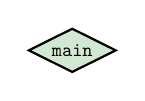
\begin{tikzpicture}[baseline=(textnode.base)]
				\node[
				draw=black,
				line width=0.8pt,
				fill=ForestGreen!20,
				text=black,
				diamond,
				aspect=2,
				inner sep=2pt,
				scale=0.7
				] (textnode) {\texttt{main}};
			\end{tikzpicture}
			&\!\!\rightarrow\!\!&
			\begin{array}{c}
				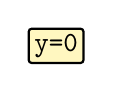
\begin{tikzpicture}[baseline=(ybox.base)]
					\node[
					draw=black,
					line width=0.8pt,
					fill=brightyellow,
					text=black,
					rectangle,
					rounded corners=1pt,
					inner sep=2pt
					] (ybox) {\texttt{y=0}};
				\end{tikzpicture}\vspace{-2pt}
				\\
				\begin{minipage}{0.20\linewidth}
					\begin{lstlisting}[language=CustomPseudoCode,numbers=none,basicstyle=\tiny\ttfamily]
X := 1 
yield 
y := X
X := 0
return y
					\end{lstlisting}
				\end{minipage}
			\end{array}
		\end{array}
		\big]
		\big\}
		\\[2em]
		resp \coloneq &
		\big\{
		\big[
		\begin{array}{c c c}
			\begin{array}{c}
				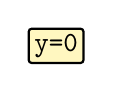
\begin{tikzpicture}[baseline=(ybox.base)]
					\node[
					draw=black,
					line width=0.8pt,
					fill=brightyellow,
					text=black,
					rectangle,
					rounded corners=1pt,
					inner sep=2pt
					] (ybox) {\texttt{y=0}};
				\end{tikzpicture}\vspace{-2pt}
				\\
				\begin{minipage}{0.11\linewidth}
					\begin{lstlisting}[language=CustomPseudoCode,numbers=none,basicstyle=\tiny\ttfamily]
return y
					\end{lstlisting}
				\end{minipage}
			\end{array}
			&\!\!\rightarrow\!\!&
			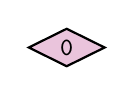
\begin{tikzpicture}[baseline=(textnode.base),scale=0.7]
				\node[
				draw=black,
				line width=0.8pt,
				fill=RedViolet!20,
				text=black,
				diamond,
				aspect=2,
				inner sep=2pt,
				font=\small
				] (textnode) {\texttt{0}};
			\end{tikzpicture}
		\end{array}
		\big]\,{},
		\big[
		\begin{array}{c c c}
			\begin{array}{c}
				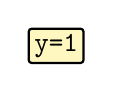
\begin{tikzpicture}[baseline=(ybox.base)]
					\node[
					draw=black,
					line width=0.8pt,
					fill=brightyellow,
					text=black,
					rectangle,
					rounded corners=1pt,
					inner sep=2pt
					] (ybox) {\texttt{y=1}};
				\end{tikzpicture}\vspace{-2pt}
				\\
				\begin{minipage}{0.11\linewidth}
					\begin{lstlisting}[language=CustomPseudoCode,numbers=none,basicstyle=\tiny\ttfamily]
return y
					\end{lstlisting}
				\end{minipage}
			\end{array}
			&\!\!\rightarrow\!\!&
			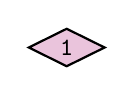
\begin{tikzpicture}[baseline=(textnode.base),scale=0.7]
				\node[
				draw=black,
				line width=0.8pt,
				fill=RedViolet!20,
				text=black,
				diamond,
				aspect=2,
				inner sep=2pt,
				font=\small
				] (textnode) {\texttt{1}};
			\end{tikzpicture}
		\end{array}
		\big]
		\big\}
		\\[2em]
		\delta \coloneq & 
		\big\{\big[(
		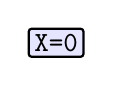
\begin{tikzpicture}[baseline=(ybox.base)]
			\node[
			draw=black,
			line width=0.8pt,
			fill=blue!10,
			text=black,
			rectangle,
			rounded corners=1pt,
			inner sep=2pt
			] (ybox) {\texttt{X=0}};
		\end{tikzpicture}\,{},
		\begin{array}{c}
			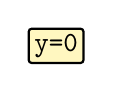
\begin{tikzpicture}[baseline=(ybox.base)]
				\node[
				draw=black,
				line width=0.8pt,
				fill=brightyellow,
				text=black,
				rectangle,
				rounded corners=1pt,
				inner sep=2pt
				] (ybox) {\texttt{y=0}};
			\end{tikzpicture}\vspace{-2pt}
			\\
			\begin{minipage}{0.14\linewidth}
				\begin{lstlisting}[language=CustomPseudoCode,numbers=none,basicstyle=\tiny\ttfamily]
X := 1
yield
y := X
X := 0
return y
				\end{lstlisting}
			\end{minipage}
		\end{array}
		)
		\;\rightarrow\;
		(
		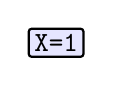
\begin{tikzpicture}[baseline=(ybox.base)]
			\node[
			draw=black,
			line width=0.8pt,
			fill=blue!10,
			text=black,
			rectangle,
			rounded corners=1pt,
			inner sep=2pt
			] (ybox) {\texttt{X=1}};
		\end{tikzpicture}\,{},
		\begin{array}{c}
			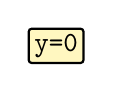
\begin{tikzpicture}[baseline=(ybox.base)]
				\node[
				draw=black,
				line width=0.8pt,
				fill=brightyellow,
				text=black,
				rectangle,
				rounded corners=1pt,
				inner sep=2pt
				] (ybox) {\texttt{y=0}};
			\end{tikzpicture}\vspace{-2pt}
			\\
			\begin{minipage}{0.14\linewidth}
				\begin{lstlisting}[language=CustomPseudoCode,numbers=none,basicstyle=\tiny\ttfamily]
y := X
X := 0
return y
				\end{lstlisting}
			\end{minipage}
		\end{array}
		)
		\big],
		\\[0.5em]
		& \phantom{\big\{}
		\big[(
		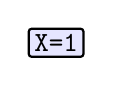
\begin{tikzpicture}[baseline=(ybox.base)]
			\node[
			draw=black,
			line width=0.8pt,
			fill=blue!10,
			text=black,
			rectangle,
			rounded corners=1pt,
			inner sep=2pt
			] (ybox) {\texttt{X=1}};
		\end{tikzpicture}\,{},
		\begin{array}{c}
			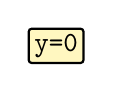
\begin{tikzpicture}[baseline=(ybox.base)]
				\node[
				draw=black,
				line width=0.8pt,
				fill=brightyellow,
				text=black,
				rectangle,
				rounded corners=1pt,
				inner sep=2pt
				] (ybox) {\texttt{y=0}};
			\end{tikzpicture}\vspace{-2pt}
			\\
			\begin{minipage}{0.14\linewidth}
				\begin{lstlisting}[language=CustomPseudoCode,numbers=none,basicstyle=\tiny\ttfamily]
y := X
X := 0
return y
				\end{lstlisting}
			\end{minipage}
		\end{array}
		)
		\;\rightarrow\;
		(
		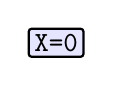
\begin{tikzpicture}[baseline=(ybox.base)]
			\node[
			draw=black,
			line width=0.8pt,
			fill=blue!10,
			text=black,
			rectangle,
			rounded corners=1pt,
			inner sep=2pt
			] (ybox) {\texttt{X=0}};
		\end{tikzpicture}\,{},
		\begin{array}{c}
			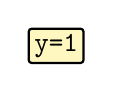
\begin{tikzpicture}[baseline=(ybox.base)]
				\node[
				draw=black,
				line width=0.8pt,
				fill=brightyellow,
				text=black,
				rectangle,
				rounded corners=1pt,
				inner sep=2pt
				] (ybox) {\texttt{y=1}};
			\end{tikzpicture}
			\vspace{-2pt}
			\\
			\begin{minipage}{0.11\linewidth}
				\begin{lstlisting}[language=CustomPseudoCode,numbers=none,basicstyle=\tiny\ttfamily]
return y
				\end{lstlisting}
			\end{minipage}
		\end{array}
		)
		\big],
		\ldots
		\big\}
	\end{array}
	\]
	\caption{The \(\delta\) transition function, and the \(req\) and \(resp\) mappings for the program in Listing~\ref{lst:MotivatingExample2NonSer}.}
	\label{fig:code2ExampleNSSecondPart}
\end{figure}



\begin{figure}[!htbp]
	\centering
	%–––– Network system diagram ––––
	% \includegraphics[width=\textwidth]{plots/code_2_NS.png}\\[1ex]

	\begin{tikzpicture}[
		node distance=1.5cm and 2.5cm,
		>=stealth,
		thick,
		every node/.style={font=\small}
	]
	  % [main request] -> [y=0][full program below that] ---[X=1 -> X=1][X=0 -> X=1 below that]--->[y=0][rest of program below that]
	  %   (first outgoing edge of last node on previous line)
      %   --[X=0 -> X=0]-->[y=0][empty program below that] ---> [0 response]
	  %   (second outgoing edge)
	  %   --[X=1 -> X=0]-->[y=1][empty program below that] ---> [1 response]
	  
	  % Main request node
	  \node[
		draw=black,
		line width=0.8pt,
		fill=ForestGreen!20,
		text=black,
		diamond,
		aspect=2,
		inner sep=2pt,
		scale=0.7
	  ] (main) {\texttt{main}};
	  
	  % First state node with full program
	  \node[right=0.7cm of main, align=center] (state1) {
		\begin{tikzpicture}[baseline=(ybox.base)]
			\node[
			draw=black,
			line width=0.8pt,
			fill=brightyellow,
			text=black,
			rectangle,
			rounded corners=1pt,
			inner sep=2pt
			] (ybox) {\texttt{y=0}};
		\end{tikzpicture}\\[-2.5pt]
		\begin{minipage}{1.0cm}
			\begin{lstlisting}[language=CustomPseudoCode,numbers=none,basicstyle=\tiny\ttfamily]
X := 1
yield
y := X
X := 0
return y
			\end{lstlisting}
		\end{minipage}
	  };
	  
	  % Second state node with rest of program
	  \node[right=of state1, align=center] (state2) {
		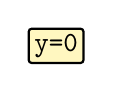
\begin{tikzpicture}[baseline=(ybox.base)]
			\node[
			draw=black,
			line width=0.8pt,
			fill=brightyellow,
			text=black,
			rectangle,
			rounded corners=1pt,
			inner sep=2pt
			] (ybox) {\texttt{y=0}};
		\end{tikzpicture}\\[-2.5pt]
		\begin{minipage}{1.0cm}
			\begin{lstlisting}[language=CustomPseudoCode,numbers=none,basicstyle=\tiny\ttfamily]
y := X
X := 0
return y
			\end{lstlisting}
		\end{minipage}
	  };
	  
	  % Final state y=0 with empty program
	  \node[above right=-0.5cm and 2.2cm of state2, align=center] (state3) {
		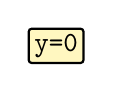
\begin{tikzpicture}[baseline=(ybox.base)]
			\node[
			draw=black,
			line width=0.8pt,
			fill=brightyellow,
			text=black,
			rectangle,
			rounded corners=1pt,
			inner sep=2pt
			] (ybox) {\texttt{y=0}};
		\end{tikzpicture}\\[-2.5pt]
		\begin{minipage}{1.0cm}
			\begin{lstlisting}[language=CustomPseudoCode,numbers=none,basicstyle=\tiny\ttfamily]
return y
			\end{lstlisting}
		\end{minipage}
	  };
	  
	  % Final state y=1 with empty program
	  \node[below right=-0.2cm and 2.2cm of state2, align=center] (state4) {
		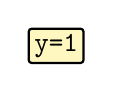
\begin{tikzpicture}[baseline=(ybox.base)]
			\node[
			draw=black,
			line width=0.8pt,
			fill=brightyellow,
			text=black,
			rectangle,
			rounded corners=1pt,
			inner sep=2pt
			] (ybox) {\texttt{y=1}};
		\end{tikzpicture}\\[-2.5pt]
		\begin{minipage}{1.0cm}
			\begin{lstlisting}[language=CustomPseudoCode,numbers=none,basicstyle=\tiny\ttfamily]
return y
			\end{lstlisting}
		\end{minipage}
	  };
	  
	  % Response 0
	  \node[
		right=0.6cm of state3,
		draw=black,
		line width=0.8pt,
		fill=RedViolet!20,
		text=black,
		diamond,
		aspect=2,
		inner sep=2pt,
		scale=0.7,
		font=\Large
	  ] (resp0) {\texttt{0}};
	  
	  % Response 1
	  \node[
		right=0.6cm of state4,
		draw=black,
		line width=0.8pt,
		fill=RedViolet!20,
		text=black,
		diamond,
		aspect=2,
		inner sep=2pt,
		scale=0.7,
		font=\Large
	  ] (resp1) {\texttt{1}};
	  
	  % Arrows
	  \draw[->] (main) -- (state1);
	  
	  % Transition labels for state1 to state2
	  \draw[->] (state1) -- node[above] {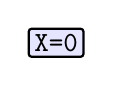
\begin{tikzpicture}[baseline=(a.base)]\node[draw=black,line width=0.8pt,fill=blue!10,rectangle,rounded corners=1pt,inner sep=2pt] (a) {\texttt{X=0}};\end{tikzpicture} $\to$ 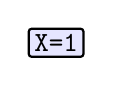
\begin{tikzpicture}[baseline=(b.base)]\node[draw=black,line width=0.8pt,fill=blue!10,rectangle,rounded corners=1pt,inner sep=2pt] (b) {\texttt{X=1}};\end{tikzpicture}} node[below] {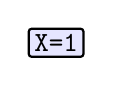
\begin{tikzpicture}[baseline=(c.base)]\node[draw=black,line width=0.8pt,fill=blue!10,rectangle,rounded corners=1pt,inner sep=2pt] (c) {\texttt{X=1}};\end{tikzpicture} $\to$ 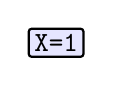
\begin{tikzpicture}[baseline=(d.base)]\node[draw=black,line width=0.8pt,fill=blue!10,rectangle,rounded corners=1pt,inner sep=2pt] (d) {\texttt{X=1}};\end{tikzpicture}} (state2);
	  
	  % From state2 to final states
	  \draw[->] ([yshift=4pt]state2.east) to[out=50,in=180] node[above, sloped] {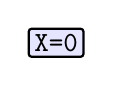
\begin{tikzpicture}[baseline=(a.base)]\node[draw=black,line width=0.8pt,fill=blue!10,rectangle,rounded corners=1pt,inner sep=2pt] (a) {\texttt{X=0}};\end{tikzpicture} $\to$ 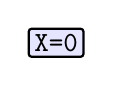
\begin{tikzpicture}[baseline=(b.base)]\node[draw=black,line width=0.8pt,fill=blue!10,rectangle,rounded corners=1pt,inner sep=2pt] (b) {\texttt{X=0}};\end{tikzpicture}} (state3.west);
	  \draw[->] ([yshift=-16pt]state2.east) to[out=-50,in=180] node[below, sloped] {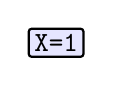
\begin{tikzpicture}[baseline=(a.base)]\node[draw=black,line width=0.8pt,fill=blue!10,rectangle,rounded corners=1pt,inner sep=2pt] (a) {\texttt{X=1}};\end{tikzpicture} $\to$ 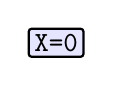
\begin{tikzpicture}[baseline=(b.base)]\node[draw=black,line width=0.8pt,fill=blue!10,rectangle,rounded corners=1pt,inner sep=2pt] (b) {\texttt{X=0}};\end{tikzpicture}} (state4.west);
	  
	  % To responses
	  \draw[->] (state3) -- (resp0);
	  \draw[->] (state4) -- (resp1);
	  
	\end{tikzpicture}
	\caption{
	The network system from the translated \toolname{} program in Listing~\ref{lst:MotivatingExample2NonSer}. 
	Local states (depicted by yellow rectangles \fcolorbox{black}{brightyellow}{\rule{0pt}{7pt}\rule{7pt}{0pt}}) present the request-local variable assignments coupled with the remaining code; edges indicate transitions of global states  (depicted by blue rectangles \fcolorbox{black}{blue!10}{\rule{0pt}{7pt}\rule{7pt}{0pt}}). 
	The request and response labels are denoted by {\color{ForestGreen!20}$\blacklozenge$} (green) and
		{\color{RedViolet!20}$\blacklozenge$} (red) diamonds, respectively.
		From left to right: a request label ${\color{ForestGreen}\blacklozenge_{\text{main}}}$ spawns a new request with initial local variable assignment \texttt{[y=0]} coupled with the full, remaining program to execute; after yielding, the $\delta$ transition steps with global state \texttt{[X=1]} and local state \texttt{[y=0]}, and subsequently updates the local variable \texttt{y} based on the global value of \texttt{[X]}, which is then returned as the final response to the user (either as {\color{red}$\blacklozenge_0$} or as {\color{red}$\blacklozenge_1$}).
		}
		%
%	\caption{The Network system for Listing~\ref{lst:MotivatingExample2NonSer}. 
%		Local states include (\textcolor{orange}{yellow}) local variable assignments and the remaining program; edges are labeled with (\textcolor{blue}{blue}) global state transitions. 
%		Requests and responses are shown as \textcolor{ForestGreen}{green} and \textcolor{red}{red} diamonds, respectively. 
%		From left to right: a \texttt{main} request spawns a thread with \texttt{[y=0]} and the full program; after yielding, $\delta$ advances to a step with global \texttt{[X=1]} and local \texttt{[y=0]} plus the remaining three expressions,; \texttt{y} is updated based on the global value, and \texttt{y}'s final assignment is the returned response.}

%		Network system for the program in Listing~\ref{lst:MotivatingExample2NonSer}. Local states consist of local variable assignments and a remaining program. Edges in the NS are labeled with their corresponding global state transition(s). Requests and responses are diamonds. 
	%
%	From left to right: a \texttt{main} request spawns a thread with \texttt{[y=0]} and the full program; after yielding, the $\delta$ transitions to a step in which  (globally) \texttt{[X=1]} and (locally) \texttt{[y=0]} with the remaining three expressions, etc.
	%	
%	For the explicit schemes of \(\delta\), \(req\), and \(resp\) see Appendix~\ref{appendix:delta-req-resp-examples}.
%}
\label{fig:code2ExampleNS}
\end{figure}



	 \section{Formal Results}
\label{sec:formal-results}

%\begin{itemize}
%	\item Results that we rely on (petri nets, semilinear sets)
%	\item The base algorithm described in math (without any optimizations)
%	\item Time complexity
%	\item proof for correctness of bidirectional pruning
%	\item mathematical description of optimizations
%\end{itemize}




\subsection{The Algorithm (without Optimizations)}

Given a network system, defined as \(\mathcal S= (G, L, \mathit{REQ},  \mathit{RESP}, g_0, \delta, \mathit{req}, \mathit{resp})\), our decision procedure runs the following steps:  

%\begin{enumerate}
%	\item  
\medskip
	\noindent
	\textbf{Step 1: Serializability automaton.} 
	We define the following NFA 
	\(
	\mathcal A_{\mathrm{ser}}(\mathcal S)=(Q,\Sigma,\delta^A,q_0,F)
	\), with
	\( Q=G,\;F=G,\;q_0=g_0,
	\)
	over the alphabet of all request/response pairs
	\(
	\Sigma=\{({\color{ForestGreen}\blacklozenge_{\mathit{req}}}/{\color{red}\blacklozenge_{\mathit{resp}}})
	\mid {\color{ForestGreen}\blacklozenge_{\mathit{req}}}\in\mathit{REQ},\;
	{\color{red}\blacklozenge_{\mathit{resp}}}\in\mathit{RESP}\}.
	\)
%	
%	\todo{old}
%	We define an NFA
%	\[
%	\mathcal A_{\mathrm{ser}}(\mathcal S)
%	= \bigl(Q,\Sigma,\delta,q_0,F\bigr),
%	\quad
%	Q = G,\quad F = G \;\;(\text{global states}),\quad
%	q_0 = g_0 \;\;(\text{initial state}),
%	\]
%	\[
%	\Sigma
%	= \Bigl\{
%	({\color{ForestGreen}\blacklozenge_{\mathit{req}}}\,/\,%
%	{\color{red}\blacklozenge_{\mathit{resp}}})
%	\;\Big|\;
%	{\color{ForestGreen}\blacklozenge_{\mathit{req}}}\in\mathit{REQ},\;
%	{\color{red}\blacklozenge_{\mathit{resp}}}\in\mathit{RESP}
%	\Bigr\}.
%	\]
%
Each transition of the NFA corresponds to a single character, i.e., a single request/response pair:
\(
\delta^A \subseteq Q \times \Sigma \times Q,
\quad q \xrightarrow{{\color{ForestGreen}\blacklozenge_{\mathit{req}}}/{\color{red}\blacklozenge_{\mathit{resp}}}} q'
\),
%old
%\(
%\delta \;\subseteq\; Q \times \Sigma_{	{\color{ForestGreen}\blacklozenge_{\mathit{req}}}\,/\,%
%	{\color{red}\blacklozenge_{\mathit{resp}}}} \times Q,
%\quad
%\bigl(q \xrightarrow{%
%	{\color{ForestGreen}\blacklozenge_{\mathit{req}}}\,/\,%
%	{\color{red}\blacklozenge_{\mathit{resp}}}%
%} q'\bigr),
%\)
%
%\;\Longleftrightarrow\;
%\begin{array}{l}
iff network system $\mathcal S$ is in global state $q$ and issues a request
$	{\color{ForestGreen}\blacklozenge_{\mathit{req}}}$, then upon some \textit{full serial execution} of $	{\color{ForestGreen}\blacklozenge_{\mathit{req}}}$ the network system finally transitions to the global state  $q'$ and returns to the user the response $	{\color{red}\blacklozenge_{\mathit{resp}}}$.
%\end{array}
%\]
%
%
%
%
%
%
%\begin{array}{l}
%	\mathcal S \text{ at global state } q
%	\;\text{issues}\;
%	{\color{ForestGreen}\blacklozenge_{\mathit{req}}},\\[0.5ex]
%	\text{after full completion of the request, it receives}\;
%	{\color{red}\blacklozenge_{\mathit{resp}}},\\[0.5ex]
%	\text{arriving at global state } q'
%\end{array}
%\]
%
%	
The NFA's language
	\(L(\mathcal A_{\mathrm{ser}}(\mathcal S))\subseteq\Sigma^*\) is the set of
	request/response traces induced by serial executions, from any reachable global state.
	Hence, by definition, applying the Parikh image on this regular language induces the (infinite) set of all (order-less) multisets of request/response pairs that are obtained by serial executions:
	\(
	\mathsf{Ser}(\mathcal S)
	\;=\;
	\mathsf{Parikh}\bigl(L(\mathcal A_{\mathrm{ser}}(\mathcal S))\bigr)
	\;\subseteq\;\mathbb N^{\Sigma}.
	\)
%	Finally,
%	\(
%	q_0 = g_0
%	\quad\text{(the initial global state of the NS)}
%	\).
	
	
%	\smallskip
\begin{tcolorbox}[colback=black!5!white, colframe=black, boxrule=1pt]
	\textbf{Example.} For Listing~\ref{lst:MotivatingExample2NonSer}, the network system in Fig.~\ref{fig:code2ExampleNS} gives rise to the Serial NFA that is presented in Fig.~\ref{fig:code2ExampleNFA}.
	%
	A trace of request/response pairs is accepted by the NFA iff there exists a serial execution of the network system that induces it.
	%	
In this case, serial executionsinduce only ({\color{ForestGreen}$\blacklozenge_\text{main}$}/{\color{red}$\blacklozenge_1$}), and the only reachable global state is [\texttt{X=0}].
%	Due to the aforementioned construction, a string of request/response pairs is accepted by the NFA iff there exists a serial execution of the NS that induces it.
%
%	As the states encode the global variable values, and the edges encode request/response pairs for all serial executions, the  
%Specifically, in this case --- serial executions can only produce request/response pairs of the type ({\color{ForestGreen}$\blacklozenge_\text{main}$/{\color{red}$\blacklozenge_1$}}). Furthermore, the only global state reachable in serial executions, is [\texttt{X=0}]. 
	%
%	Intuitively, this corresponds to [\texttt{X=0}] being the initial global state, as well as the system's global state after every single packet exits the network in a serial execution.
	\end{tcolorbox}
	%
%	\begin{figure}[!htbp]
%		\centering
%		% 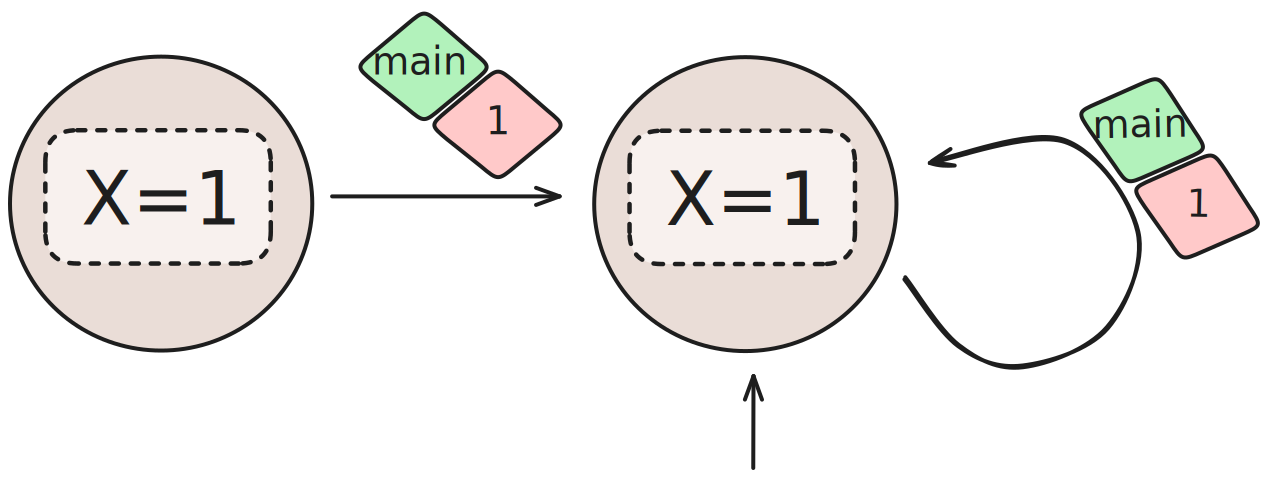
\includegraphics[width=0.48\textwidth,trim=0 0 0 0,clip]{plots/code_2_NFA_v3.pdf}
%		
%		\begin{tikzpicture}[
%			->,>=stealth,
%			thick,
%			node distance=2.5cm,
%			state/.style={
%				draw=black,
%				line width=0.8pt,
%				fill=blue!10,
%				rectangle,
%				rounded corners=1pt,
%				inner sep=2pt,
%				font=\small
%			},
%			every node/.style={font=\small}
%			]
%			% States using the same notation as section 3
%			\node[state] (X1) {\texttt{X=1}};
%			\node[state, right of=X1] (X0) {\texttt{X=0}};
%			
%			% Initial state arrow
%			\draw[->] ([yshift=-0.4cm]X0.south) -- (X0.south);
%			
%			% Transitions with proper colored notation from the paper
%			\draw[->] (X1) -- node[above] {${\color{ForestGreen}\blacklozenge_{\mathrm{main}}}/{\color{red}\blacklozenge_1}$} (X0);
%			\draw[->] (X0) edge[loop right] node[right] {${\color{ForestGreen}\blacklozenge_{\mathrm{main}}}/{\color{red}\blacklozenge_1}$} (X0);
%		\end{tikzpicture}
%		
%		\caption{Serial NFA of Listing~\ref{lst:MotivatingExample2NonSer}.}
%		\label{fig:code2ExampleNFA}
%	\end{figure}
	
	\begin{figure}[!htbp]
		\centering
		
		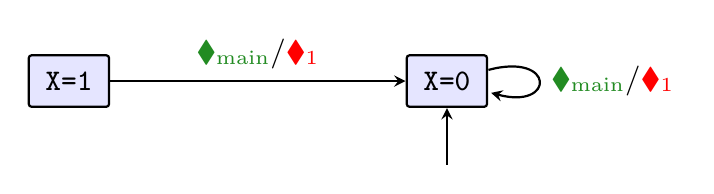
\begin{tikzpicture}[
			scale=1.2, transform shape,  % Scales the entire diagram and text
			->,>=stealth,
			thick,
			node distance=4cm, % Increased distance for better spacing
			state/.style={
				draw=black,
				line width=0.8pt,
				fill=blue!10,
				rectangle,
				rounded corners=1pt,
				inner sep=5pt, % Slightly more padding
				font=\small
			},
			every node/.style={font=\small}
			]
			% States using the same notation as section 3
			\node[state] (X1) {\texttt{X=1}};
			\node[state, right of=X1] (X0) {\texttt{X=0}};
			
			% Initial state arrow
			\draw[->] ([yshift=-0.6cm]X0.south) -- (X0.south);
			
			% Transitions with proper colored notation from the paper
			\draw[->] (X1) -- node[above] {${\color{ForestGreen}\blacklozenge_{\mathrm{main}}}/{\color{red}\blacklozenge_1}$} (X0);
			\draw[->] (X0) edge[loop right] node[right] {${\color{ForestGreen}\blacklozenge_{\mathrm{main}}}/{\color{red}\blacklozenge_1}$} (X0);
		\end{tikzpicture}
		
		\caption{Serial NFA of Listing~\ref{lst:MotivatingExample2NonSer}.}
		\label{fig:code2ExampleNFA}
	\end{figure}

	
%	\begin{wrapfigure}{r}{0.50\textwidth}  % “r” = right, width = 0.5\textwidth
%		\centering
%		% 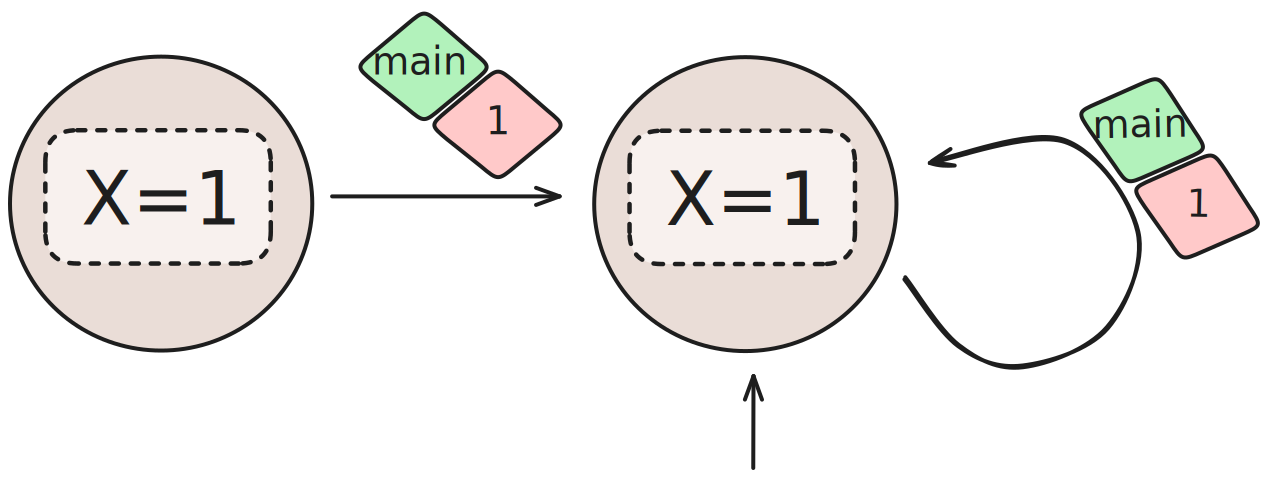
\includegraphics[width=0.48\textwidth,trim=0 0 0 0,clip]{plots/code_2_NFA_v3.pdf}
%		
%		\begin{tikzpicture}[
%			->,>=stealth,
%			thick,
%			node distance=2.5cm,
%			state/.style={
%				draw=black,
%				line width=0.8pt,
%				fill=blue!10,
%				rectangle,
%				rounded corners=1pt,
%				inner sep=2pt,
%				font=\small
%			},
%			every node/.style={font=\small}
%			]
%			% States using the same notation as section 3
%			\node[state] (X1) {\texttt{X=1}};
%			\node[state, right of=X1] (X0) {\texttt{X=0}};
%			
%			% Initial state arrow
%			\draw[->] ([yshift=-0.4cm]X0.south) -- (X0.south);
%			
%			% Transitions with proper colored notation from the paper
%			\draw[->] (X1) -- node[above] {${\color{ForestGreen}\blacklozenge_{\mathrm{main}}}/{\color{red}\blacklozenge_1}$} (X0);
%			\draw[->] (X0) edge[loop right] node[right] {${\color{ForestGreen}\blacklozenge_{\mathrm{main}}}/{\color{red}\blacklozenge_1}$} (X0);
%		\end{tikzpicture}
%		
%		\caption{Serial NFA of Listing~\ref{lst:MotivatingExample2NonSer}.}
%		\label{fig:code2ExampleNFA}
%	\end{wrapfigure}
	%
	%
	%Intuitively, this corresponds to the Listing~\ref{lst:MotivatingExample2NonSer} program updating [X:=1] as an intermediate assignment before yielding.
	
	
	
%\medskip
\noindent
%	\item 
	\textbf{Step 2: Interleaving Petri net.}
%	
Next, we translate the network system into a Petri net \(N_{\mathrm{int}}(\mathcal S)\). Each \textit{non-sink place} of the Petri net represents either a global state assignment or a local states of in-flight packets. Each \textit{sink place} represents request/response pairs of terminated packets.
%
The \textit{transitions} between states are defined to correspond to the \(\delta\), \(req\), and \(resp\) mappings of the network system. We note that the \(req\) transitions can fire without any input tokens in order to correspond to external spawning of arbitrarily-many requests.
%
Finally, we define \(M_0\) to be an initial marking encoding a single token in the non-sink place corresponding to \(g_0\), i.e., the initial global state of the network system.
%
This construction is formalized in full in  Appendix~\ref{appendix:NS-to-PN-formulation}, and guarantees that each multiset of all markings \(M\) (with \(M_0 \xrightarrow{}^{*} M\)) when projected (via \(\pi\)) to the sink places, corresponds to a multiset of (${{\color{ForestGreen}\blacklozenge_{\mathit{req}}}/{\color{red}\blacklozenge_{\mathit{resp}}}}$) pairs, as induced by a network system interleaving, i.e., \(\mathsf{Int}(\mathcal S)=\{\pi(M) \mid M \in R(N_{\mathrm{int}}(\mathcal S))\}\).



\begin{tcolorbox}[colback=black!5!white, colframe=black, boxrule=1pt]
	\textbf{Example.}
%	\textit{Notation.}
Continuing our running example, the network system induces the Petri net presented in Fig.~\ref{fig:code2ExamplePN}, encoding all possible interleavings. The places \textcolor{blue}{$P_2$} and \textcolor{blue}{$P_3$} respectively correspond to the global states \textcolor{blue}{[X=1]} and \textcolor{blue}{[X=0]}, and places $P_1$, $P_4$, $P_5$, and $P_6$ correspond to the local states of in-flight requests, i.e., the assignments to each request’s local variables, coupled with the remaining \toolname{} program code to execute. Similarly, places \textcolor{red}{$P_7$} and \textcolor{red}{$P_8$} correspond to responses {\color{red}$\blacklozenge_1$} and {\color{red}$\blacklozenge_0$}, respectively. Thus, each token models either an active (in-flight) request, a completed request/response pair, or --- when the token resides in a place denoting the global state --- the current global state of the network system. Finally, transitions are induced by the network system’s mappings ($\delta/req/resp$): they either advance the program by a single step (e.g., \(t_2,t_3,t_4,\) and \(t_5\), based on $\delta$), represent external spawning of a new request (e.g., transition $\textcolor{ForestGreen}{t_1}$, which corresponds to request {\color{ForestGreen}$\blacklozenge_{\mathrm{main}}$} based on $req$),
or return a response (e.g., transitions $\textcolor{red}{t_6}$ and $\textcolor{red}{t_7}$, based on $resp$).
\end{tcolorbox}

%Finally, the NS gives rise to the PN in Fig.~\ref{fig:code2ExamplePN}, encoding all possible interleavings.
%%
%The places represent either the global state
%(e.g., places \textcolor{blue}{$P_2$} and \textcolor{blue}{$P_3$} correspond to the global states \textcolor{blue}{[X=1]} and \textcolor{blue}{[X=0]}), while others ($P_1,P_4,P_5,P_6$) correspond to the local state of an in-flight request, i.e., combinations of ``remaining'' programs  assignments to local variables of in-flight requests.
%%
%Furthermore, some requests correspond to responses, e.g., places \textcolor{red}{$P_7$} and \textcolor{red}{$P_8$} corresponds to {\color{red}$\blacklozenge_1$} and {\color{red}$\blacklozenge_0$}.
%%
%Each token corresponds either to a single in-flight request, a single terminated pair of request/response, or (in the case of the global-variable-encoding places), to the current global state.
%%
%Finally, transitions represent the network system's $\delta$ mapping --- encoding either a ``step'' of our program, or spawning a request ($t_1$, which  corresponds to spawning {\color{ForestGreen}$\blacklozenge_\text{main}$}), or returning a response (e.g. transitions $t_6,t_7$).
%


\begin{figure}[!htbp]
	\centering
	\includegraphics[width=1.0\textwidth]{plots/code_2_PN_with_annotation_fixed.png}
	\caption{The Petri net encoding interleaved executions of the \toolname{} program in Listing~\ref{lst:MotivatingExample2NonSer}.}
	\label{fig:code2ExamplePN}
\end{figure}


	\clearpage
%	\pagebreak
%	\medskip
	\noindent
%	\item 
	\textbf{Step 3: Non-serializable set.}  
	We define
	\(\;\mathsf{NonSer}(\mathcal S)=\mathbb N^{|\Sigma|}\setminus \mathsf{Ser}(\mathcal S)\), i.e., the (possibly empty) set of all multisets of (${{\color{ForestGreen}\blacklozenge_{\mathit{req}}}/{\color{red}\blacklozenge_{\mathit{resp}}}}$) pairs that \textit{cannot} be obtained by any serial execution of the network system $\mathcal S$.
	
	\begin{tcolorbox}[colback=black!5!white, colframe=black, boxrule=1pt]
	\textbf{Example.}
	In our running example, we automatically generate the following reachability query\footnote{Note that, if not for the equality constraints, the problem would have been a PN \textit{coverability} query, which is easier~\cite{Ra78} that general reachability.} for the Petri net presented in Fig.~\ref{fig:code2ExamplePN}. The query encodes a target semilinear set by imposing on the tokens the following constraints:
	%
	%Regarding the aforementioned program, we automatically generate the following reachability query~\footnote{If not the equality constraints, the problem would have been considered a \textit{coverability} query which is easier~\cite{Ra78}.} for the Petri net in Figure~\ref{fig:code2ExamplePN} we encode a target semilinear set with the following constraints on the token distribution:
	%
	\[
	\mathcal {F}: \quad P_1 = 0 \wedge 
	\textcolor{blue}{P_2} \ge 0 \wedge \textcolor{blue}{P_3} \ge 0  \wedge P_4 = 0
	\wedge P_5 = 0 \wedge P_6 = 0 \wedge \textcolor{red}{P_7} \ge 0 \wedge \textcolor{red}{P_8} \ge 1.
	\]
	
	Specifically, this constrains places $P_1,P_4,P_5,P_6$ to include no tokens, and requires at least a single token on place $\textcolor{red}{P_8}$ (which corresponds to response {\color{red}$\blacklozenge_0$}). Furthermore, there are no constraints on the token count
	of places $\textcolor{blue}{P_2},\textcolor{blue}{P_3},\textcolor{red}{P_7}$. 
	%
%	Note that \(\textcolor{red}{P_8} \ge 1\) requires at least one {\color{red}$\blacklozenge_0$}, as expected (see \Cref{sec:introduction}).
	\end{tcolorbox} 
	
	
%	\item \textbf{Reachability encoding.}  
	
	\medskip
	\noindent
%	\item 
	\textbf{Step 4: Decision \& validation.}
	Finally, after encoding the Petri net and the reachability query, we ask whether there \textit{exists} a reachable marking \(M\) of \(N_{\mathrm{int}}(\mathcal S)\) such that \(M \models \mathcal {F}\) holds. As \(\mathcal {F}\) encodes \(\mathsf{NonSer}(\mathcal S)\), this is equivalent to obtaining a marking \(M\) such that \(	M_0 \xrightarrow{}^{*} M\) and also
	\[
	\pi(M) \in \mathsf{Int}(\mathcal S)
	\quad\wedge\quad
	\pi(M)\in \mathsf{NonSer}(\mathcal S).
	\]
	
	\begin{itemize}
		\item [\sat]: induces a counterexample interleaving \(M\) with
		\(\pi(M)\notin \mathsf{Ser}(\mathcal S)\), which can further be validated by simulating the network system \(\mathcal S\).
%		We validate a reachable trace and embed it into the NS semantics, yielding a valid interleaving that produces request/response pairs unattainable under any serial execution.
		
		\item [\unsat]: induces an inductive invariant of
		\(N_{\mathrm{int}}(\mathcal S)\), which we then back-translate to a network-system-level proof of serializability 
%		(Appendix~\ref{appendix:ns-serializable}).
%		
%		which back-translates to an NS-level proof of
%		serializability 
%		for \(\mathcal S\)
		%
%		back-translated to a validated by synthesizing an inductive invariant over the interleaving PN, thereby proving that the corresponding semilinear set cannot be realized by any interleaving 
(see an example of such a proof in Appendix~\ref{appendix:ns-serializable}).
	\end{itemize}

\begin{tcolorbox}[colback=black!5!white, colframe=black, boxrule=1pt]
	\textbf{Example.}
	In the running example, the target semilinear set \(\mathcal {F}\) is reachable (this is not surprising, as it corresponds to a non-serial \toolname{} program). For examples, the following marking is included in \(\mathcal {F}\):
	
	\[
	M^* = \{\textcolor{blue}{P_3}(1),\;\textcolor{red}{P_7}(1),\;\textcolor{red}{P_8}(1)\}
	\]
	
and is also reachable by the Petri net depicted in Fig.~\ref{fig:code2ExamplePN}. 
%
We also present in Table~\ref{tab:PetriNetFiringCounterexample} the full, step-by-step firing sequence leading to marking $M^*$.
	%
%	As the target set encodes request/response pairs that are \textit{unattainable} via serial executions, and as the PN encodes all possible interleavings, this firing sequence also corresponds as a counterexample demonstrating the program is non-serializable. 
	%
	Specifically, this reachable marking encodes $\{{\color{ForestGreen}\blacklozenge_\text{main}}/{\color{red}\blacklozenge_0},{\color{ForestGreen}\blacklozenge_\text{main}}/{\color{red}\blacklozenge_1}\}$ which, indeed, can only be induced by a non-serial execution of Listing~\ref{lst:MotivatingExample2NonSer}.
\end{tcolorbox} 




\begin{table}[!htbp]
	\centering
	%
	\small
	\begin{tabular}{c l c c c c c c}
		\toprule
		\textbf{Step} 
		& \textbf{Firing} 
		& \multicolumn{3}{c}{\textbf{Marking (after firing)}} 
		& \multicolumn{3}{c}{\textbf{Description (after firing)}} \\
		\cmidrule(lr){3-5} \cmidrule(lr){6-8}
		& & \textbf{Global} & \textbf{Local} & \textbf{Responses} 
		& \textbf{Global state} & \textbf{In-flight requests} & \textbf{Responses} \\
		\midrule
		0 & -- & {\color{blue}$P_3$(1)} & -- & -- & {\color{blue}[X=0]} & -- & -- \\
		\midrule
		1 & $\textcolor{ForestGreen}{t_1}$ & {\color{blue}$P_3$(1)} & $P_1$(1) & -- & {\color{blue}[X=0]} & {\color{ForestGreen}$\blacklozenge_\text{main}$} & -- \\
		\midrule
		2 & $\textcolor{ForestGreen}{t_1}$ & {\color{blue}$P_3$(1)} & $P_1$(2) & -- & {\color{blue}[X=0]} & \begin{tabular}[t]{@{}c@{}}{\color{ForestGreen}$\blacklozenge_\text{main}$}, \\ {\color{ForestGreen}$\blacklozenge_\text{main}$}\end{tabular} & -- \\
		\midrule
		3 & $t_3$ & {\color{blue}$P_2$(1)} & \begin{tabular}[t]{@{}c@{}}$P_1$(1),\\$P_4$(1)\end{tabular} & -- & {\color{blue}[X=1]} & \begin{tabular}[t]{@{}c@{}}{\color{black}$\blacklozenge_\text{until yield}$},\\{\color{ForestGreen}$\blacklozenge_\text{main}$}\end{tabular} & -- \\
		\midrule
		4 & $t_2$ & {\color{blue}$P_2$(1)} & $P_4$(2) & -- & {\color{blue}[X=1]} & \begin{tabular}[t]{@{}c@{}}{\color{black}$\blacklozenge_\text{until yield}$},\\{\color{black}$\blacklozenge_\text{until yield}$}\end{tabular} & -- \\
		\midrule
		5 & $t_4$ & {\color{blue}$P_3$(1)} & \begin{tabular}[t]{@{}c@{}}$P_5$(1),\\$P_4$(1)\end{tabular} & -- & {\color{blue}[X=0]} & \begin{tabular}[t]{@{}c@{}}{\color{black}$\blacklozenge_\text{after yield}$},\\{\color{black}$\blacklozenge_\text{until yield}$}\end{tabular} & -- \\
		\midrule
		6 & $\textcolor{red}{t_6}$ & {\color{blue}$P_3$(1)} & $P_4$(1) & {\color{red}$P_7$(1)} & {\color{blue}[X=0]} & {\color{black}$\blacklozenge_\text{until yield}$} & {\color{red}$\blacklozenge_1$} \\
		\midrule
		7 & $t_5$ & {\color{blue}$P_3$(1)} & $P_6$(1) & {\color{red}$P_7$(1)} & {\color{blue}[X=0]} & {\color{black}$\blacklozenge_\text{after yield}$} & {\color{red}$\blacklozenge_1$} \\
		\midrule
		8 & $\textcolor{red}{t_7}$ & {\color{blue}$P_3$(1)} & -- & \begin{tabular}[t]{@{}c@{}}{\color{red}$P_7$(1)},\\{\color{red}$P_8$(1)}\end{tabular} & {\color{blue}[X=0]} & -- & \begin{tabular}[t]{@{}c@{}}{\color{red}$\blacklozenge_0$},\\{\color{red}$\blacklozenge_1$}\end{tabular} \\
		\bottomrule
	\end{tabular}
	\caption{The firing sequence reaching marking $M^*$ which is in our target semilinear set $\mathcal{F}$. 
		The marking $P_i(n_j)$ indicates that there are $n_j$ tokens in place $P_i$. 
		The initial marking has a single token in place \textcolor{blue}{$P_3$}, encoding $g_0$ (\textcolor{blue}{[X=0]}).}
	\label{tab:PetriNetFiringCounterexample}
\end{table}



%\item \textbf{Validation.}  
%
%	\begin{itemize}
%		
%		\item[\sat]: 
%		See the example in subsec.~\ref{subsec:ns-not-serializable}.
%		
%%		\item[\unsat]: 
%		
%		
%	\item \sat: we validate the reachable trace and project it to the NS semantics to represent a valid interleaving that results into request/response pairs which cannot be attained in serial executions.
%	See example in subsec.~\ref{subsec:ns-not-serializable}.
	
%	\item \unsat:
%	we generate an inductive invariant over the interleaving PN, proving that the semilinear set cannot be attained via an interleaving.
%	See example in subsec.~\ref{subsec:ns-serializable}.
%\end{itemize}

%\end{enumerate}

%\medskip
%\noindent
%\textbf{Complexity analysis.}
%\clearpage
\subsection{Complexity Analysis}

Our core decision procedure reduces serializability to checking Petri net reachability over a target semilinear set. 
As the serial executions form a regular language (step 1), their Parikh image is semilinear by Parikh's theorem, with size that is exponential in the NFA.
The PN encoding the interleavings (step 2) has $O(|G| + (|\mathit{REQ}| \times |L|) + (|\mathit{REQ}| \times |\mathit{RESP}|))$ places and has $O(|\mathit{REQ}|\times (1+ |\delta| + |\mathit{RESP}|))$ transitions.
The reachability query (step 3) asks whether the Petri net can reach a marking in the semilinear set of the outputs that cannot be obtained by non-serial executions. This is decidable, but with \texttt{Ackermann}-complete~\cite{CzWo22,Le22} complexity.
Thus, without further optimizations, even simple examples can generate queries that are intractable in practice. 
Our optimizations (see \Cref{sec:optimizations}) \textit{drastically} reduce both the time and space complexity, as elaborated next.


%\guy{should we add/prove the following?}
%
%\begin{proposition}
%	Let $N_{\mathrm{int}}(\mathcal S)=(P,T,\mathsf{pre},\mathsf{post},M_0)$ be the interleaving Petri net constructed above, and let
%	\[
%	\pi\colon\mathbb N^P\to\mathbb N^{P_R}
%	\]
%	be the projection onto the request/response places $P_R$.  Then
%	\[
%	\mathsf{Int}(\mathcal S)
%	\;=\;
%	\{\;\pi(M)\;\mid\;M_0\xrightarrow{*}M\}.
%	\]
%\end{proposition}


	 \todo{from here}
	 \section{Optimizations}
\label{sec:optimizations}


%\todo{check}

We apply four optimizations to the base algorithm to control intermediate blow‐up in the size of both the PN and the constructed semilinear set. 
%
An extensive empirical evaluation of these optimizations appears in Appendix~\ref{appendix:full_results}.

%\medskip
%\noindent
%\textbf{(1) Bidirectional slicing.} 
\subsection{Bidirectional slicing} 
When solving Petri net reachability, many places and transitions might be irrelevant to the specific target set~\cite{Ra12}.  
	We slice them before symbolic reasoning by combining forward and backward passes:  
	the forward pass over-approximates the places reachable from $M_0$; and symmetrically,   
	the backward pass traverses in reverse from any place that can influence a target constraint (hence over-approximating the places that can contribute to it).
	We iteratively remove non-forward-reachable and
	non-backward-relevant places and transitions, to a fixed point.  
	This process is illustrated in Fig.~\ref{fig:bidirectional_pruning}, and its soundness is proven in Theorem~\ref{thm:bidirectional-pruning}.




\begin{figure}[h]
	\centering
	
	% Top row: (a), (b)
	\begin{subfigure}[b]{0.45\textwidth}
		\centering
		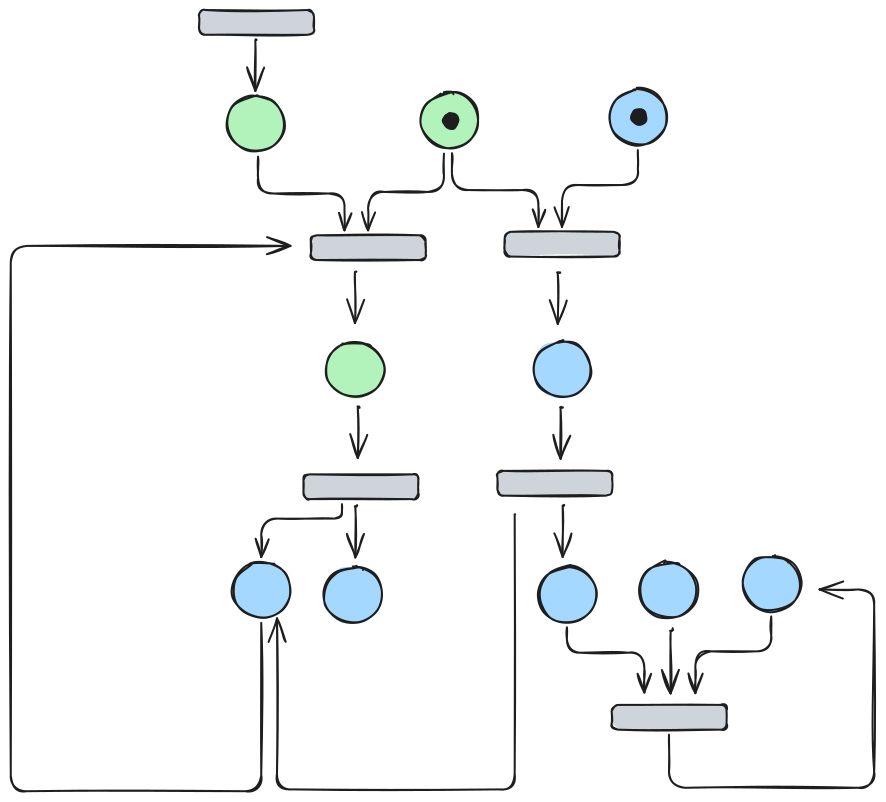
\includegraphics[width=\textwidth]{plots/bidirectional_pruning_step_a_updated.pdf}
		\caption{Step 0: initial Petri net, before slicing.}
		\label{fig:step:a}
	\end{subfigure}\hfill
	\begin{subfigure}[b]{0.45\textwidth}
		\centering
		\includegraphics[width=\textwidth]{plots/bidirectional_pruning_step_b_updated.pdf}
		\caption{Step 1: first forward pass.}
		\label{fig:step:b}
	\end{subfigure}
	
	\vspace{1em}
	
	% Bottom row: (c), (d), (e)
	\begin{subfigure}[b]{0.30\textwidth}
		\centering
		\includegraphics[width=\textwidth]{plots/bidirectional_pruning_step_c_updated.pdf}
		\caption{Step 2: first backward pass.}
		\label{fig:step:c}
	\end{subfigure}\hfill
	\begin{subfigure}[b]{0.23\textwidth}
		\centering
		\includegraphics[width=\textwidth]{plots/bidirectional_pruning_step_d_updated_2.pdf}
		\caption{Step 3: second forward pass.}
		\label{fig:step:d}
	\end{subfigure}\hfill
	\begin{subfigure}[b]{0.23\textwidth}
		\centering
		\includegraphics[width=\textwidth]{plots/bidirectional_pruning_step_e_updated_2.pdf}
		\caption{Step 4: final Petri net.}
		\label{fig:step:e}
	\end{subfigure}
	
	\caption{A Petri net during three rounds of bidirectional slicing: two forward passes and one backward pass. Black dots represent initial token markings; green places represent places that are allowed to be reachable in our constraints (i.e., aren't fixed to zero tokens in the final marking). Dashed shapes represent places and transitions that are identified as removable in the current iteration, and will be removed after it ends.}
	\label{fig:bidirectional_pruning}
\end{figure}


%\guy{check with mark (M0 projected on P or P'?)}

\begin{theorem}[Bidirectional Slicing Soundness]
	\label{thm:bidirectional-pruning}
	Let $N = (P, T, \Pre, \Post, M_0)$ be a Petri net and $S$ a target set.  
	Let $N' = (P',T',\,\Pre|_{P'\times T'},\,\Post|_{P'\times T'},\,M_0|_{P'})$ be the sliced net.  
	Then $S$ is reachable from $N$ iff it is reachable from $N'$.
\end{theorem}
%
%We depict this in Fig.~\ref{fig:bidirectional_pruning}, and prove Theorem~\ref{thm:bidirectional-pruning} in Appendix~\ref{appendix:BidirectionalProof}.
% (see the proof in Appendix~\ref{appendix:BidirectionalProof}).
%

% \medskip
% \noindent\textit{\textbf{Intuition.}}
% Before any heavy symbolic reasoning takes place, we apply bidirectional pruning on the underlying PN.  In the forward pass, we traverse from the initial marking to identify an over-approximation of all places and transitions that could ever fire; in the backward pass, we traverse backward from any place that can influence a target constraint, and identify over-approximations on transitions and places that cannot contribute to reaching it.  By iteratively repeating forward passes and backward passes until convergence, we remove every component of the net that cannot both originate and contribute to the reachable target set.  This dramatically shrinks the net in practice, often converting an intractably large model into one small enough for exhaustive analysis.

%\medskip
%\noindent
\subsection{Semilinear set pruning}  
A semilinear set $S=\bigcup_{i=1}^m L_i$ with 
	$L_i=\{\,\mathbf{b}_i+\sum_{\mathbf{p}\in P_i}n_p \mathbf{p} \mid n_p\in\mathbb N\}$ may contain redundant 
	period vectors or components.  
	Thus, during construction, we:
	(1) remove any period vector $\mathbf{p}\in P_i$ expressible as a nonnegative combination of $P_i\setminus\{\mathbf{p}\}$; 
	and (2) drop $L_i$ when $L_i\subseteq L_j$ (for \(i \neq j\)).  
	This pruning keeps formulas compact and solver calls tractable.




% it is common for some inequalities or disjuncts to add no new coverage beyond what other constraints already guarantee.  The redundant‐constraint elimination pass inspects each linear inequality and each disjunct in a disjunctive normal form, testing whether it is implied by the rest.  Any constraint or disjunct found redundant is dropped, ensuring that subsequent intersection, union, and projection operations work on the smallest necessary formula.  This streamlines the logic formula and prevents unnecessary size blow‐ups during solver invocations.

% %
% We replace each period‐basis \(P_i\) by
% \[
% P_i \;:=\;\{\,p\in P_i \mid p\notin\mathsf{Span}(P_i\setminus\{p\})\}
% \],
% Dropping any ``redundant'' periods, and removing any \(L_j\subseteq L_i\) for \(i\neq j\), iterating to a fixed point so no two components subsume one another.

%\medskip
%\noindent
\subsection{Generating fewer constraints}  
When computing the Parikh image of a regular expression as a semilinear set,
	most regex operations can be implemented without an exponential blow-up.
	However, the Kleene star is a notable exception. Given $S=\bigcup_{i=1}^m L_i$,  the Kleene closure $S^\ast$ can be expressed as a semilinear set by: 
	\[
	S^\ast=\bigcup_{I \subseteq \{1,...,m\}} 
	\Big\{\sum_{i \in I} \mathbf{b}_i + \sum_{\mathbf{p} \in \bigcup_{i \in I} (P_i\cup \{\mathbf{b}_i\})} n_p \mathbf{p}\Big\},
	\]
	yielding $2^m$ components. To mitigate this:
	(i) if $L_i=\{\mathbf{b}_i\}$ (period-less component), factor it out, star the rest, then add $\mathbf{b}_i$ as a period;  
	(ii) if $L_i=\{\sum_{\mathbf{p}\in P_i}n_p\mathbf{p}\}$ (zero base), likewise star the rest and add each $\mathbf{p}\in P_i$ as a period vector to the resulting set.  
	Each such case halves the component count and circumvents exponential blow-ups.




% Let $\mathrm{comp}(S)=\{L_1,\dots,L_m\}$ 
% be the multiset of linear components of the semilinear set 
% \(\displaystyle S=\bigcup_{i=1}^m L_i\), where each 
% \(\;L_i=b_i+\langle P_i\rangle\) with \(b_i\in\mathbb N^d\) and 
% \(P_i\subseteq\mathbb N^d\).  Define the pruning operator
% \[
% \mathrm{new}(\mathcal C)
% \;=\;
% \bigcup\bigl\{\,L\in\mathcal C \;\bigm|\;\nexists\,L'\in\mathcal C\setminus\{L\}:\;L'\subsetneq L\bigr\},
% \]
% which removes any component strictly containing another.  
% %
% \guy{Nicolas is it clear we mean that we fix their semilinear "meaning" of the regex operations? For example, + is union etc..}
% Then, we replace the naive semilinear‐set operations by
% \[
% S\;+\;T
% \;=\;
% \mathrm{new}\bigl(\mathrm{comp}(S)\,\cup\,\mathrm{comp}(T)\bigr),
% \]
% \[
% S\;\cdot\;T
% \;=\;
% \mathrm{new}\Bigl(\{\,L_i\cdot L'_j \mid L_i\in\mathrm{comp}(S),\;L'_j\in\mathrm{comp}(T)\}\Bigr),
% \]
% where for
% \(\;L_i=b_i+\langle P_i\rangle,\;L'_j=b'_j+\langle P'_j\rangle\) we set
% $
% L_i\cdot L'_j
% =\;(b_i+b'_j)\;+\;\langle\,P_i\cup P'_j\,\rangle.
% $
% Finally, for Kleene‐star and plus on the regex side one similarly applies
% \(\mathrm{new}(\cdot)\) to the collection of ``folded” components instead of
% building all intermediate ones:
% \[
% S^*
% =\mathrm{new}\Bigl(\bigcup_{k\ge0}\bigl(\mathrm{comp}(S)\bigr)^k\Bigr),
% \qquad
% S^+
% =S\cdot S^*.
% \]

% \medskip
% \noindent\textit{\textbf{Intuition.}}
% %
% During set construction --- especially when introducing new existentially‐quantified variables or combining transition effects, we selectively avoid generating any marking that would strictly dominate an already‐seen solution.  In effect, whenever a candidate disjunct would yield a superset of an existing one, it is skipped entirely.  This ``generate‐less” heuristic stops the proliferation of large, overlapping regions in the semilinear description.  In benchmarks with large state spaces, it can reduce the number of intermediate branches by orders of magnitude.

%\medskip
%\noindent
\subsection{Strategic Kleene elimination order} 
%
We use \textit{Kleene's algorithm}~\cite{Kl56} to translate the serializability NFA into a regex.
% 
The size of the generated semilinear set is not only impacted by how the
	semilinear set operations are implemented, but also by what \textit{specific} regular
	expression is given as input: a single regular language may be represented by a
	number of equivalent regexes, each of different complexity.
	%
	In particular, as Kleene star can cause a large blow-up in the semilinear set size,
	we are especially sensitive to the \emph{star height} of the generated regex.
	%
	Naive Kleene elimination may introduce many nested stars.  
	We reduce this by strategically choosing to eliminate lower-degree states first:
	\[
	q^*=\arg\min_{q\in Q}\bigl(|\delta^A_{\mathrm{in}}(q)|+|\delta^A_{\mathrm{out}}(q)|\bigr).
	\]
	 
	
	\smallskip
	\noindent
	As we demonstrate in Appendix~\ref{appendix:full_results}, our optimizations expedite the search procedure and make the representations \textit{significantly} more compact. This, in turn, enables deciding serializability for instances that are otherwise intractable.


%\medskip
%\noindent
%\textbf{(4) Strategic Kleene elimination order.}  
%The size of the generated semilinear set is not only impacted by how the
%semilinear set operations are implemented, but also by what specific regular
%expression is given as input: a single regular language may be represented by a
%number of equivalent regexes, each of different complexity.
%%
%In particular, as Kleene star can cause a large blow-up in the semilinear set size,
%we are especially sensitive to the \emph{star height} of the generated regex.
%%
%We use Kleene's algorithm to convert an NFA $\mathcal A=(Q,\Sigma,\delta,q_0,F)$ to a regex, which works by repeated state elimination, choosing one state at a time.
%Naively, when eliminating states in an arbitrary order, Kleene's algorithm may generate regexes with a much greater star height than necessary---a problem
%when converting to semilinear sets.
%%
%Therefore, we heuristically optimize the state elimination order to end up with a smaller regex. Formally, we pick the next state:
%\[
%q^* = 
%\arg\min_{q\in Q'}\bigl(|\delta_{\mathrm{in}}(q)|+|\delta_{\mathrm{out}}(q)|\bigr)
%\]
%where \(Q'\subseteq Q\) are the states remaining to be eliminated, choosing to
%eliminate states with a smaller total degree first.
%%
%This empirically keeps the resulting regexes small.

% \medskip
% \noindent\textit{\textbf{Intuition.}}
% When converting an NFA to a single regex, we pick the next state to eliminate by heuristically choosing the  state with the fewest incoming and outgoing edges.
% This optimization allows for circumventing 
% overblown expressions resulting in naive translations, especially with regard to  Kleene closures (the “\(\mathsf{*}\)” operator).  Instead, we analyze the structure of sub-expressions under the various operators --- estimating their branching factor, and reordering them so that simpler, low‐branching components are expanded first.  
%This adaptive ordering often leads to early detection of fixed points or dead‐ends, preventing the combinatorial explosion that arises when complex loops are expanded prematurely.  

	 

\section{Implementation}
\label{sec:implementation}

%\begin{wraptable}[11]{r}{0.32\textwidth}
%	\vspace{-1.5em} 
%	\centering
%	\begin{tabular}{@{} l S[table-format=5.0] @{}}
%		\toprule
%		\textbf{Module}                & {\textbf{LoC}} \\
%		\midrule
%		Input \& Parsing               &  1723          \\
%		Model Construction             &  5561          \\
%		Petri--Net Conversion           &   843          \\
%		Reachability          &  2628          \\
%		Proof Checking                 &  3240          \\
%		Utilities                      &  2160          \\
%		Testing \& Evaluation          &  2118          \\
%		\midrule
%		\textbf{Total}                 & \textbf{18273} \\
%		\bottomrule
%	\end{tabular}
%	\caption{Lines of Code}
%	\label{tab:loc_summary2}
%\end{wraptable}
%\vspace{-1.5\baselineskip} % nudge following text up a bit
%We implemented our approach in \toolname{}~\cite{ArtifactRepository}, a publicly available toolchain 
%%consisting of over $18{,}200$ LoC 
%written mostly in \texttt{Rust}. 
%(see Table~\ref{tab:loc_summary2})
%
%
%We next elaborate on the architecture of our tool and the various optimizations we added to allow it to run efficiently.
%For the underlying Petri Net model checker, we use SMPT~\cite{AmDa23},though other off-the-shelf solvers can be used as well.
%For the underlying Petri Net model checker, we use SMPT~\cite{AmDa23} which supports \textit{unbounded} reachability queries (see Appendix~\ref{appendix:smpt}).
%, and which uses Z3 as an underlying SMT solver~\cite{DeBj08}. 
%and which we extended to support our setting (for example, we needed to extend the solver to support proof generation). 
%
%We note that other off-the-shelf solvers can be used as well.

%The implementation..

%\begin{enumerate}
%	\item The extra things we did to make the thing actually run
%	\item Code architecture
%	\item Optimizations
%\end{enumerate}

%\newpage
\subsection{Code Architecture}

%\begin{tabular}{|l|r|}
%	\hline
%	\textbf{Module} & \textbf{LoC} \\
%	\hline
%	Input \& Parsing                             & 1723  \\
%	\hline
%	Model Construction                           & 5561  \\
%	\hline
%	Petri-Net Conversion                         & 843   \\
%	\hline
%	Reachability Checking                        & 2628  \\
%	\hline
%	Proof Checking                               & 3240  \\
%	\hline
%	Utilities                                       & 2160  \\
%	\hline
%	Testing \& Evaluation               & 2118  \\
%	\hline
%	\textbf{Total}                               & \textbf{18273} \\
%	\hline
%\end{tabular}


%
%\begin{table}[ht]
%	\centering
%	\label{tab:loc_summary}
%	\begin{tabular}{@{} l S[table-format=5.0] @{}}
%		\toprule
%		\textbf{Module}                & {\textbf{LoC}} \\
%		\midrule
%		Input \& Parsing               &  1723          \\
%		Model Construction             &  5561          \\
%		Petri–Net Conversion           &   843          \\
%		Reachability Checking          &  2628          \\
%		Proof Checking                 &  3240          \\
%		Utilities                      &  2160          \\
%		Testing \& Evaluation          &  2118          \\
%		\midrule
%		\textbf{Total}                 & \textbf{18273}          \\
%		\bottomrule
%	\end{tabular}
%	\caption{Lines of Code by Module}
%\end{table}
%

% Then, where you want the table wrapped to the right:
%
% this table summarizes the values without whitespaces/comments and without the code for SMPT (or the wrapper) or the carfo and toml files
%
%\begin{wraptable}[8]{r}{0.32\textwidth}
%	\centering
%	\begin{tabular}{@{} l S[table-format=5.0] @{}}
%		\toprule
%		\textbf{Module}                & {\textbf{LoC}} \\
%		\midrule
%		Input \& Parsing               &  1723          \\
%		Model Construction             &  5561          \\
%		Petri–Net Conversion           &   843          \\
%		Reachability          &  2628          \\
%		Proof Checking                 &  3240          \\
%		Utilities                      &  2160          \\
%		Testing \& Evaluation          &  2118          \\
%		\midrule
%		\textbf{Total}                 & \textbf{18273} \\
%		\bottomrule
%	\end{tabular}
%	\caption{Lines of Code (LoC)}
%	\label{tab:loc_summary2}
%\end{wraptable}
%
%\noindent

Our decision procedure is implemented in \toolname{}~\cite{ArtifactRepository}, a publicly available toolchain 
%consisting of over $18{,}200$ LoC 
written mostly in \texttt{Rust}. 
%
The toolchain receives an input program (which can be written in the \toolname{} syntax), and runs the end-to-end serializability checker on it. If the program is serializable, the toolchain returns a network-system level proof thereof; otherwise, if it is not serializable, the toolchain provides a counterexample, i.e., a specific interleaving that induces a multiset of request/response pairs that cannot be obtained in \textit{any} serial execution.
%
Our toolchain reduces the problem of deciding the networks system's serializability to an equivalent Petri net reachability problem over an unbounded number of tokens. Our construction guarantees that (i) the Petri net represents every possible request/response multiset that is induced by an interleaving of the original program; and (ii) the reachability query encodes multisets of request/response pairs that \textit{cannot} be induced by serial executions.
%
In order to cope with the \texttt{Ackermann}-completeness of unbounded Petri net reachability~\cite{CzWo22,Le22}, we implemented the various optimizations that expedite the search procedure, both at the Petri net level, and also, at the property-encoding level.
%
We illustrate the pipeline of \toolname{} in Fig.~\ref{fig:full_program_flow}. Furthermore, \toolname{} includes the following modules:
 

\begin{enumerate}
	\item \textbf{Input \& parsing.} 
	Our toolchain receives as input either a \toolname{} program with the syntax described in~\Cref{sec:problem-definition}, or alternatively, a \texttt{JSON} file that directly encodes a network system. In the case of the former, the toolchain does an additional step in which it parses the input %(using the \texttt{parser.rs} module) 
	to an expression tree that is then translated into the equivalent network system.
%	, represented as a struct in the \texttt{ns.rs} module. 
	
	\item \textbf{Petri net conversion.} The network system is subsequently translated into a Petri net 
%	(see the \texttt{petri.rs} module) 
representing all possible interleavings of the original program as depicted, for example, in Fig.~\ref{fig:code2ExamplePN}.
	Each place represents a state (either global or local) or a response. Each token that is not in a place encoding a global state, represents a single in-flight request or a terminated response. 
Furthermore, we note that the Petri net is encoded in the de facto standard \texttt{NET} format, to allow support by off-the-shelf Petri net model checkers. 
	
	\item \textbf{Semilinear conversion.} 
%	This includes a set of modules (\texttt{kleene.rs}, \texttt{semilinear.rs}, and \texttt{presburger.rs}) which 
We construct a semilinear set that encodes all the request/response multisets that cannot be induced by any serial exection.
This step is done via translation of the serialized NFA (e.g., Fig.~\ref{fig:code2ExampleNFA}) to a regular expression, which is then projected (using the Parikh image) and complemented. 
%	This conversion is done by the following pipeline: (1) the NS is translated to an NFA encoding all possible request/response pairs of the input program; (2) This NFA is translated to a regex (via Kleene's Theorem) and then projected (via the Parikh Image) to a semilinear set. The (finite) encoding of the semilinear set symbolically represents all outputs attained via serializable executions of the program, running for an unbounded number of steps; (3) finally, we complement the semilinear set to encode all outputs unattainable via serial executions. 
	After this stage, our toolchain generates an \texttt{XML}-formatted file encoding a reachability query over the token distribution of the Petri net.
	
	
	\item \textbf{Reachability engine.} Both the Peri net and the accompanying reachability query are fed to a Petri net model checker, which combines techniques such as \textit{bounded model checking} (BMC)~\cite{BiCiClZh99} in search of a counterexample; and \textit{state equation reasoning}~\cite{Mu77} in order to prove non-reachability. 
%	This engine is implemented in the \texttt{reachability.rs} and \texttt{reachability\_with\_proofs.rs}  modules.
	%
	Furthermore, in order to curtail the search space, we replace ``large'' (Petri net, reachability query) pairs with multiple sliced Petri nets, with each sliced Petri net coupled with a sub-query encoding a separate disjunct in the original, full query. 
%	of the original query.
	We iteratively solve the 
	disjuncts on the fly, until either \texttt{SAT} is reached, in which case, we have a concrete counterexample; or otherwise, if all disjuncts are found to be \texttt{UNSAT}, we deduce that the original program is serializable.
	
	
	\item \textbf{Proof \& certification.} 
	If the query is \texttt{SAT}, we reconstruct the reachable marking and validate a network-system level counterexample. Otherwise, if the query is \texttt{UNSAT}, we extract an inductive, per-disjunct proof for non-satisfiability, and then ``stitch'' these to a single inductive serializability certificate. This certificate is then projected to the network system, over which we validate (i) initiation, (ii) inductiveness, and (iii) query refutation.
	%
%	If the query is \texttt{SAT}, we reconstruct a non-serializable NS-level execution and validate its correctness. Otherwise, if all disjuncts are \texttt{UNSAT}, our proof module extracts a separate proof for each disjunct. We subsequently ``stitch'' these proofs to a single inductive invariant, and project it to the NS-level, representing a full inductive proof certificate for serializability. Our checker also validates that the inductive invariant is correct, i.e., (i) includes the initial state; (ii) is inductive with regard to the transitions; and (iii) implies that the reachability query is \texttt{UNSAT}.
	%, and hence, implying serializability. 
	
	
	\item \textbf{Instrumentation \& logging.} Throughout execution, we record various 
%	intermediate representations and performance metrics.  
	input size and performance metrics, such as number of places, transitions, constraint complexity, timings and more.
%
%
We generate \texttt{CSV} and \texttt{JSON} analysis logs, and we also assemble 
an \texttt{HTML} report embedding the original net, symbolic constraints, reachability results, proofs, etc.

\item \textbf{Debug report generation.} Finally, a human-readable \texttt{HTML} report is assembled: it embeds the original net, symbolic constraints, reachability results, proof outlines, and profiling graphs. This interactive report allows users to drill down into each transition firing, constraint check, and proof obligation.
	
	\item \textbf{Output delivery.} The toolchain exposes a simple CLI and library API. Users obtain either a Boolean reachability verdict, raw log files, or a full \texttt{HTML} debug report, depending on invocation flags.
	
%	\item \textbf{Optimizations.} As formalized in the previous section, we implement multiple optimizations throughout the process.
%	, both for representing the semilinear sets succinctly and for pruning the Petri Nets. These optimizations significantly reduce the search space and expedite the model-checking process.
\end{enumerate}



%\noindent
%This linear pipeline - \emph{parse} -> \emph{model} -> \emph{normalize} -> \emph{analyze} -> \emph{prove} -> \emph{report} --- ensures a clear separation of concerns, easy extensibility (e.g., swapping backends), and comprehensive traceability from input to certified result.```


\begin{figure}[!htbp]
	\centering
	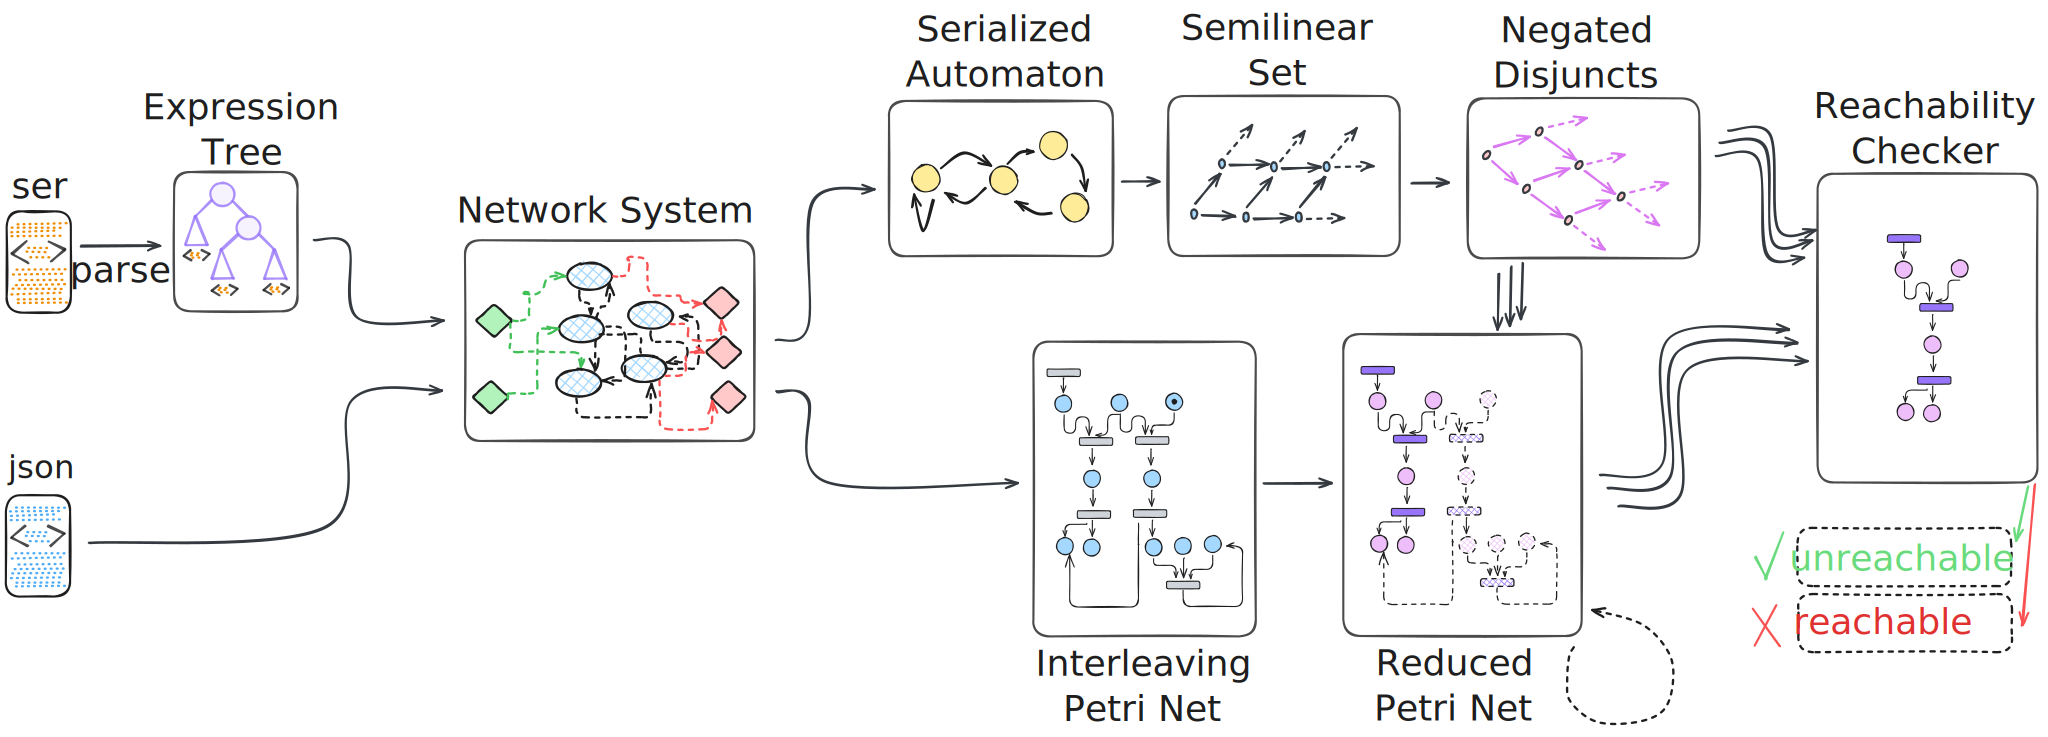
\includegraphics[width=1.0\textwidth]{plots/full_program_flow.pdf}
	\caption{The full decision procedure scheme 
%		If the target set is unreachable --- a serializability proof is produced; otherwise, if it is reachable --- a counterexample trace is generated.
	(simplified version, excluding backward arrows 
%	translating invariants (if serializable) or counterexample traces (if non-serializable) back 
	to the network system level).}
	\label{fig:full_program_flow}
\end{figure}


%\subsection{Optimizations}

%\paragraph{Bidirectional Pruning of the Petri Net}
%Before any heavy symbolic reasoning takes place, we apply bidirectional pruning on the underlying PN.  In the forward pass, we traverse from the initial marking to identify all places and transitions that could ever fire; in the backward pass, we traverse backward from any place that can influence a target constraint, and identify transitions and places that cannot contribute to reaching it.  By iteratively repeating forward passes and backward passes until convergence, we remove every component of the net that cannot both originate and contribute to the reachable target set.  This dramatically shrinks the net in practice, often converting an intractably large model into one small enough for exhaustive analysis.
%%
%We depict this in Fig.~\ref{fig:bidirectional_pruning}, and give a formal proof of correctness in Appendix~\ref{appendix:BidirectionalProof}.

%\paragraph{Redundant‐Constraint Elimination}
%When manipulating Presburger sets or their semilinear representations, it is common for some inequalities or disjuncts to add no new coverage beyond what other constraints already guarantee.  The redundant‐constraint elimination pass inspects each linear inequality and each disjunct in a disjunctive normal form, testing whether it is implied by the rest.  Any constraint or disjunct found redundant is dropped, ensuring that subsequent intersection, union, and projection operations work on the smallest necessary formula.  This streamlines the logic formula and prevents exponential blow‐up of case distinctions during solver invocations.
%
%Every time you build or star a semilinear set, you prune out any “period” vectors that are rendered useless by earlier steps:. nce you’ve accumulated a bunch of LinearSet components, you try to merge any that mathematically subsume one another:

%\paragraph{Generating Fewer Constraints}
%During set‐construction--- especially when introducing new existentially‐quantified variables or combining transition effects, we selectively avoid generating any marking that would strictly dominate an already‐seen solution.  In effect, whenever a candidate disjunct would yield a superset of an existing one, it is skipped entirely.  This ``generate‐less” heuristic stops the proliferation of large, overlapping regions in the semilinear description, trading off completeness of intermediate case‐enumeration for concise final representations.  In benchmarks with large state‐spaces, it can reduce the number of intermediate branches by orders of magnitude.

%in both the Regex and SemilinearSet Kleene-algebra instances. Concretely, instead of always building the full new structure and pruning it later, operations like union (plus) and concatenation (times) do a quick check for trivial cases and drop “zero” or “one” elements on the spo

%\paragraph{Executing Kleene Elimination in a Strategic Order:}
%When converting an NFA to a single regex, we pick the next state to eliminate by heuristically choosing the  state with the fewest incoming and outgoing edges.
%This optimization allows circumventing 
%overblown expressions resulting in naive translations, especially with regard to  Kleene closures (the “\(\mathsf{*}\)” operator).  Instead, we analyze the structure of sub-expressions under the various operators --- estimating their branching factor, and reorder them so that simpler, low‐branching components are expanded first.  This adaptive ordering often leads to early detection of fixed points or dead‐ends, preventing the combinatorial explosion that arises when complex loops are expanded prematurely.  



\subsection{SMPT}
For the underlying Petri net model checker, we use \texttt{SMPT}~\cite{AmDa23}, though other off-the-shelf solvers can be used as well.
%
\texttt{SMPT} incorporates a portfolio of symbolic model checking techniques --- including bounded model checking (BMC)~\cite{BiCiClZh99}, state equation reasoning~\cite{Mu77}, $k$-induction~\cite{BeDaWe18,ShSiSt20}, property directed reachability (PDR)~\cite{Br11,AmDaHu22,ViGu14,BjGa15,BlLa23,CiGrMoTo14,CiGrMoTo16,DuRo17}, and random state space exploration. It acts as a front-end to an \texttt{SMT} solver (\texttt{Z3}~\cite{DeBj08}, although other solvers could also be used, e.g., \texttt{cvc5}~\cite{BaCoDeHaJoKiReTi11,BaBaBrKrLaMaMoMoNiNo22}, \texttt{MathSAT}~\cite{CiGrScSe13}, etc.), while also incorporating domain-specific knowledge from Petri net theory, such as invariants and structural properties. \texttt{SMPT} has also participated in the last five editions of the \textit{Model Checking Contest} (MCC), an international competition for model-checking tools. In its most recent participation, it achieved a bronze medal and a confidence level score of  $\texttt{100\%}$, indicating it never returned an incorrect verdict~\cite{mcc:2025}.

\medskip
\noindent
\texttt{SMPT} distinguishes itself from other tools in two ways that are particularly relevant to our setting and motivate its adoption. First, to the best of our knowledge, it is the only model checker for Petri nets that provides a proof of its verdict, regardless of the underlying verification technique. This means it either produces a witness trace when the property is reachable, or, more interestingly, a certificate of non-reachability~\cite{AmDaHu22} when the property is found to be unreachable.
%
The second distinguishing feature relates to our ongoing work on polyhedral reductions~\cite{AmBeDa21,amat2022polyhedral}, as elaborated further in~\Cref{sec:discussion}.


\subsection{Benchmarks} 
\label{subsec:benchmarks}
To the best of our knowledge, ours is the first and only tool capable of (i) checking serializability on programs running \textit{unbounded} threads; and (ii) \textit{proving that serializability holds}.
%
Thus, we have found a lack of standard serializability benchmarks for evaluating our tool. Towards this end, we bridged this gap in the literature by assembling a suite of dozens of benchmarks (which we also uploaded online~\cite{ArtifactRepository}).
% additional part (from rebuttal to R4) - END
%Typically, automatically generated $\toolname$ programs do not represent real-world applications or recognizable concurrency patterns. Thus, 
We believe that this is the first benchmark suite for serializability, and includes instances of \toolname{} programs that are motivated by practical, real-world analogues.
% additional part (from rebuttal to R4) - END
Specifically, our suite includes both \texttt{SER} and \texttt{JSON} formatted programs, with both serializable and non-serializable instances.
%
Furthermore, our benchmarks (see Table~\ref{tab:benchmarks-all}) cover a broad range of features, including loops, branching, arithmetic, locks, non-determinism, and more.
%
While the benchmarks are not the paper’s primary focus, we believe they stand on their own, given their strong relevance to a range of real-world systems and applications of interest.
%
In particular, we highlight our benchmark suite encoding \textit{network \& system protocols}, which includes models of real-world BGP routing programs, stateful firewalls, asynchronous network monitors, and additional
%highlighting the serializability challenges inherent in real-world distributed programs.
%
%Here, we were motivated by 
examples motivated by real-world concurrency problems. 
%
For example, our \textit{routing-cycle benchmark} in SDN is motivated by a recent networking paper~\cite{NaGhSa24}. Another interesting example is illustrated by our \textit{snapshot isolation benchmark} --- motivated by a reported duplicate-key bug~\cite{cockroach-issue-14099} in the \texttt{CockroachDB} system~\cite{cockroachdb-si-docs}.
%
In both cases and others, the unwanted behavior was expressed by serializability violations that our toolchain successfully and automatically identified.
%
%Our benchmarks include both serializable and non-serializable instances, and their features and categorization appears in Table~\ref{tab:benchmarks-all}. 



%As there are no standard benchmarks for evaluating serializability, we wrote dozens of programs in our abstract NS language. These benchmarks span a wide range of complexity --- covering branching, looping constructs, arithmetic, non-deterministic choice, and multi-request workflows that manipulate both shared (global) variables and per-request (local) state. 
%
%We include both serializable and non-serializable instances and summarize the benchmarks' features and categorizations in Table~\ref{tab:benchmarks-all}. 
%
%In particular, our most sophisticated examples are drawn from realistic networking and system-protocol scenarios, including stateful firewalls, BGP routing, network monitoring, and more --- highlighting the serializability challenges inherent in real-world distributed programs.
%
%As there are no official benchmarks for evaluating serializability, we hand-coded dozes of programs in our abstract network-system language.
%%
%The benchmarks vary in the complexity, and have multiple features: branching, loops, arithmetic, non-determinism, and multiple requests and responses, operating on both shared (global) variables and per-request (local) variables.
%%
%The benchmarks include both serializable and non-serializable instances, as we summarize in Table.~\ref{tab:benchmarks-all}, based on a category and feature-wise breakdown.
%%
%Especially, we wish to note the final category of complex examples as motivated by real-world systems and networking programs.
%%
%These include a stateful firewall, BGP routing, network monitoring and additional examples.
%
%\begin{itemize}
%		
%	\item \todo{update benchmark overview and category names}
%	\item \textbf{Core expressions \& multi request workflows}: Benchmarks testing arithmetic, boolean, and simple control expression.
%	\item \textbf{Fred (mixed arithmetic)}: Mixed control and arithmetic transformations (Fred series).
%	\item \textbf{Stop (circular-increment) series}: Circular increment loops and variants.
%	\item \textbf{Concurrency \& locking loops}: Concurrent looping patterns with locking and tricky interactions.
%	\item \textbf{Non-deterministic choice \& randomness}: Random choice and non-deterministic branching benchmarks.
%	\item \textbf{Networking \& system protocols}: Networking protocols and system-level monitoring.
%	\item \textbf{JSON state-machine examples}: Example JSON-encoded state machine workflows.
%\end{itemize}
%
%
%
%The benchmarks differ in their complexity and in the various features pertaining to them --- branching, loops, randomness, multiple requests, etc. 
%

	

%\newpage
	 \section{Evaluation}
\label{sec:evaluation}

%\begin{enumerate}
%    \item Benchmarks (describe our benchmarks)
%    \item Results (total time, split out SMPT time from our rust code time)
%    \item Analysis of optimizations (how much time they save, petri net sizes, semilinear set sizes)
%    \item Limitations (examples we cannot solve, future work that would help)
%\end{enumerate}


\noindent
\textbf{Experimental setup.}
All experiments were run on a Lenovo ThinkPad P16s, with 16 AMD CPU cores and 64 GB of RAM, running Ubuntu 24.04.2.
%
%We plan on making all our code, benchmarks raw results publicly available with the final version of this paper.
%
We use \texttt{SMPT}~\cite{AmDa23} (built upon \texttt{Z3}~\cite{DeBj08}) as our backend Petri net model checker.
 %
Our code and benchmarks are publicly available~\cite{ArtifactRepository}.



%
\begin{table}[t]
	\vspace{-1.2\baselineskip} % pulls table upward (adjust if needed)
	\centering
	\small
	\begin{table}[H]
	\centering
	\begin{tabular}{l r r r r}
		\toprule
		& \multicolumn{2}{c}{Average (ms)} 
		& \multicolumn{2}{c}{Median (ms)} \\
		\cmidrule(lr){2-3} \cmidrule(lr){4-5}
		Category
		& \shortstack{cert.}
		& total
		& \shortstack{cert.}
		& total \\
		\midrule
		\textcolor{ForestGreen}{Serializable}      &   2{,}273 &  25{,}531 &  1{,}178 &  2{,}238 \\
		\textcolor{red}{Not serializable}  &  42{,}076 &  42{,}980 &   773 &   830 \\
		All               &  39{,}613 &  52{,}858 &   797 &  2{,}080 \\
		\bottomrule
	\end{tabular}
\end{table}

	\caption{Runtime for generating certificates (\texttt{cert.}) and the overall runtime (\texttt{total}), including for validation.}
	\label{tab:stats-summary}
	\vspace{-0.6\baselineskip} % adjusts spacing below
\end{table}
\medskip
%\subsection{Results}
\noindent
\textbf{Results.}
%
We ran \toolname{} on all 47 benchmarks, out of which 27 are serializable, and the remaining 20 are non-serializable. 
For each benchmark, we measured the time for deciding the reachability query, as well as the overall time, including validation of the invariant proof (if serializable) or of the counterexample (if not serializable). These experiments ran in parallel on $16$ cores with all four optimizations and a \texttt{TIMEOUT} threshold of $500$ seconds.
%
Within this time limit, \toolname{} solved 26 of the 27 serializable benchmarks and 19 of the 20 non-serializable benchmarks (see summary in Table~\ref{tab:stats-summary} and the full results in Table~\ref{tab:benchmarks-all}).
%
% As can be seen by our results (summarized in Table~\ref{tab:benchmarks-all}), withing this time limit, our tool fully solved 26/27 serializable benchmarks 
%and 19/20 non serializable benchmarks. 
%
The \textit{median} total runtime was $1{,}909$ ms across all benchmarks, and $2{,}238.5$ ms ($830$ ms) when  solely focusing on serializable (non-serializable) benchmarks.
%, as reported in Table~\ref{tab:stats-summary}.
%
The \textit{average} total runtime was $32{,}898.38$ ms across all benchmarks, and $25{,}530.69$ ms ($42{,}980.47$ ms) when solely focusing on serializable (non-serializable) benchmarks.
%
We also observe a clear runtime split based on serializability: 
%For serializable benchmarks, certificate validation takes much longer than proof generation. 
among non-serializable benchmarks, counterexample generation takes much longer than validation, and dominates the overall runtime; whereas among serializable benchmarks the validation time dominates the overall runtime. This is not surprising, as validating a given counterexample only requires a polynomial-time simulation of the network system to confirm its feasibility.
%
%We also note that when analyzing the benchmarks based on their serializability, there is a clear difference in their average runtime --- while in the serializable benchmarks the validation of the certificate takes significantly longer than generating the certificate (i.e., the proof) --- in the non serializable benchmarks this trend is reversed, with the overall time being dominated by the generation of the counterexample. This of course is not surprising, as counterexample generation can be done in polynomial time by emulating our network system and checking that the final counterexample can indeed be attained.
%
%We report the full results in Table~\ref{tab:stats-summary} and Table~\ref{tab:benchmarks-all}.
%, and elaborate on the per-benchmark results in Table~\ref{tab:benchmarks-all}.


%\begin{table}[!htbp]
%	\centering
%	% Load the tabular from the external file:
%	\begin{table}[H]
	\centering
	\begin{tabular}{l r r r r}
		\toprule
		& \multicolumn{2}{c}{Average time (ms)} 
		& \multicolumn{2}{c}{Median time (ms)} \\
		\cmidrule(lr){2-3} \cmidrule(lr){4-5}
		Category
		& \shortstack{certificate\\generation}
		& total
		& \shortstack{certificate\\generation}
		& total \\
		\midrule
		Serializable      &   2{,}273 &  25{,}531 &  1{,}178 &  2{,}238 \\
		Not serializable  &  42{,}076 &  42{,}980 &   773 &   830 \\
		All               &  39{,}613 &  52{,}858 &   797 &  2{,}080 \\
		\bottomrule
	\end{tabular}
\end{table}

%	\caption{Average and median runtime. Values are rounded to the nearest integer, to reduce clutter. The \textit{total} column also includes the time for validation.}
%	\label{tab:stats-summary}
%\end{table}



%\begin{table}[H]
%	\centering
%	% Load the tabular from the external file:
%	\begin{table}[H]
	\centering
	\begin{tabular}{lrrrrrr}
		\toprule
		& \multicolumn{3}{c}{Average time (ms)} & \multicolumn{3}{c}{Median time (ms)} \\
		\cmidrule(lr){2-4} \cmidrule(lr){5-7}
		Category
		& \shortstack{certificate\\generation}
		& \shortstack{certificate\\validation}
		& total
		& \shortstack{certificate\\generation}
		& \shortstack{certificate\\validation}
		& total \\
		\midrule
		Serializable      &   2273 &  23257 &  25531 &  1178 &  1300 &  2238 \\
		Not serializable  &  42076 &    905 &  42980 &   773 &    78 &   830 \\
		All               &  39613 &  13244 &  52858 &   797 &   151 &  2080 \\
		\bottomrule
	\end{tabular}
\end{table}
%\caption{Average and median runtime. Values are rounded to the nearest integer, to reduce clutter.}
%\label{tab:stats-summary}
%\end{table}





%=== Overall ===
%Certificate running time:
%Average = 39613.23
%Median  = 797.00
%
%Certificate validation time:
%Average = 13244.32
%Median  = 151.00
%
%Total running time:
%Average = 52857.55
%Median  = 2080.00
%
%=== Serializable Only ===
%Certificate running time:
%Average = 2273.38
%Median  = 1178.00
%
%Certificate validation time:
%Average = 23257.31
%Median  = 1299.50
%
%Total running time:
%Average = 25530.69
%Median  = 2238.50
%
%=== Non-Serializable Only ===
%Certificate running time:
%Average = 42075.84
%Median  = 773.00
%
%Certificate validation time:
%Average = 904.63
%Median  = 78.00
%
%Total running time:
%Average = 42980.47
%Median  = 830.00
%
%=== Percentiles (Overall) ===
%Certificate running time percentiles:
%25th percentile = 553.50
%50th percentile = 797.00
%100th percentile = 502810.00
%
%Certificate validation time percentiles:
%25th percentile = 66.50
%50th percentile = 151.00
%100th percentile = 282370.00
%
%Total running time percentiles:
%25th percentile = 615.00
%50th percentile = 2080.00
%100th percentile = 503336.00
%
%=== Percentiles (Serializable) ===
%Certificate running time percentiles:
%25th percentile = 312.00
%50th percentile = 1178.00
%100th percentile = 9858.00
%
%Certificate validation time percentiles:
%25th percentile = 115.75
%50th percentile = 1299.50
%100th percentile = 282370.00
%
%Total running time percentiles:
%25th percentile = 456.50
%50th percentile = 2238.50
%100th percentile = 292228.00
%
%=== Percentiles (Non-Serializable) ===
%Certificate running time percentiles:
%25th percentile = 628.50
%50th percentile = 773.00
%100th percentile = 356195.00
%
%Certificate validation time percentiles:
%25th percentile = 50.00
%50th percentile = 78.00
%100th percentile = 15227.00
%
%Total running time percentiles:
%25th percentile = 707.00
%50th percentile = 830.00
%100th percentile = 356299.00







%\begin{table}[t]
%	\centering
%	\small
%	\begin{table}[H] 
	\centering
	\small
	% increase horizontal padding between columns
	\setlength{\tabcolsep}{5pt}
	\renewcommand{\arraystretch}{0.9}
	\begin{tabular*}{\textwidth}{@{\extracolsep{\fill}}%
			p{2cm}     % Benchmark
			c          % Serializable
			c c c c c c % Features
			r r        % Cert, Total
		}
		\toprule
		\textbf{Benchmark}
		& \textbf{Serializable}
		& \multicolumn{6}{c}{\textbf{Features}}
		& \multicolumn{2}{c}{\textbf{Runtime (ms)}} \\
		\cmidrule(lr){1-1} \cmidrule(lr){2-2} \cmidrule(lr){3-8} \cmidrule(lr){9-10}
		& 
		& If & While & \texttt{?} & Arith & Yield & Multi-req
		& Cert. & Total \\
		\midrule
		\texttt{banking (1)}          & \xmark      & \cmark & \cmark &        & \cmark & \cmark & \cmark & 59{,}312 & 74{,}539 \\
		\texttt{banking (2)}          & \greencmark & \cmark & \cmark &        & \cmark & \cmark & \cmark & \texttt{TIMEOUT} & \texttt{TIMEOUT} \\
		\texttt{routing (1)}      & \xmark      & \cmark & \cmark & \cmark & \cmark & \cmark & \cmark & 20{,}557 & 20{,}954 \\
		\texttt{monitor (1)}       & \xmark      & \cmark & \cmark & \cmark & \cmark & \cmark & \cmark & 6{,}859  & 7{,}047 \\
		\texttt{monitor (2)}       & \greencmark & \cmark & \cmark & \cmark & \cmark & \cmark & \cmark & 3{,}047  & 12{,}324 \\
		\texttt{firewall (1)}& \xmark      & \cmark &        & \cmark & \cmark & \cmark &       & 8{,}193  & 8{,}285 \\
		\texttt{firewall (2)}& \greencmark & \cmark &        & \cmark & \cmark &       &       & 6{,}886  & 252{,}752 \\
		\midrule
		\bottomrule
	\end{tabular*}
\end{table}

%	\caption{Overview of benchmarks from the \textit{network \& system protocols} category.}
%	\label{tab:networking-benchmarks}
%\end{table}




%\begin{table}[htbp]
%	\centering
%	% Load the tabular from the external file:
%	\begin{table}[H] 
	\centering
	\small
	% increase horizontal padding between columns
	\setlength{\tabcolsep}{5pt}
	\renewcommand{\arraystretch}{0.9}
	\begin{tabular*}{\textwidth}{@{\extracolsep{\fill}}%
			p{2cm}     % Benchmark
			c          % Serializable
			c c c c c c % Features
			r r        % Cert, Total
		}
		\toprule
		\textbf{Benchmark}
		& \textbf{Serializable}
		& \multicolumn{6}{c}{\textbf{Features}}
		& \multicolumn{2}{c}{\textbf{Runtime (ms)}} \\
		\cmidrule(lr){1-1} \cmidrule(lr){2-2} \cmidrule(lr){3-8} \cmidrule(lr){9-10}
		& 
		& If & While & \texttt{?} & Arith & Yield & Multi-req
		& Cert. & Total \\
		\midrule
		\texttt{banking (1)}          & \xmark      & \cmark & \cmark &        & \cmark & \cmark & \cmark & 59{,}312 & 74{,}539 \\
		\texttt{banking (2)}          & \greencmark & \cmark & \cmark &        & \cmark & \cmark & \cmark & \texttt{TIMEOUT} & \texttt{TIMEOUT} \\
		\texttt{routing (1)}      & \xmark      & \cmark & \cmark & \cmark & \cmark & \cmark & \cmark & 20{,}557 & 20{,}954 \\
		\texttt{monitor (1)}       & \xmark      & \cmark & \cmark & \cmark & \cmark & \cmark & \cmark & 6{,}859  & 7{,}047 \\
		\texttt{monitor (2)}       & \greencmark & \cmark & \cmark & \cmark & \cmark & \cmark & \cmark & 3{,}047  & 12{,}324 \\
		\texttt{firewall (1)}& \xmark      & \cmark &        & \cmark & \cmark & \cmark &       & 8{,}193  & 8{,}285 \\
		\texttt{firewall (2)}& \greencmark & \cmark &        & \cmark & \cmark &       &       & 6{,}886  & 252{,}752 \\
		\midrule
		\bottomrule
	\end{tabular*}
\end{table}

%	\caption{Overview of benchmarks from the \textit{network \(\&\) system protocols} category. 
%%	For our full benchmarks see Appendix~\ref{appendix:full_results}.
%}
%\label{tab:networking-benchmarks}
%\end{table}





%\begin{table}[!htbp]
%	\centering
%	\begin{table}[H]
	\centering
	\begin{tabular}{l r r r r}
		\toprule
		& \multicolumn{2}{c}{Average (ms)} 
		& \multicolumn{2}{c}{Median (ms)} \\
		\cmidrule(lr){2-3} \cmidrule(lr){4-5}
		Category
		& \shortstack{cert.}
		& total
		& \shortstack{cert.}
		& total \\
		\midrule
		\textcolor{ForestGreen}{Serializable}      &   2{,}273 &  25{,}531 &  1{,}178 &  2{,}238 \\
		\textcolor{red}{Not serializable}  &  42{,}076 &  42{,}980 &   773 &   830 \\
		All               &  39{,}613 &  52{,}858 &   797 &  2{,}080 \\
		\bottomrule
	\end{tabular}
\end{table}

%	\caption{Runtime for generated certificates (\texttt{total} also includes validation).}
%	\label{tab:stats-summary}
%\end{table}

%\begin{table}[!htbp]
%	\centering
%	% Load the tabular from the external file:
%	\begin{table}[H]
	\centering
	\begin{tabular}{l c c c c}
		\toprule
		& \multicolumn{2}{c}{num components} & \multicolumn{2}{c}{periods per component} \\
		\cmidrule(lr){2-3} \cmidrule(lr){4-5}
		& mean & max & mean & max \\
		\midrule
	baseline (all ON) & 3.64 & 24 & 1.95 & 9 \\
	no\_remove\_redundant & 30.64 & 644 & \textbf{3.46} & \textbf{39} \\
	no\_generate\_less & \textbf{566.00} & \textbf{20{,}484} & 1.38 & 15 \\
	no\_smart\_order & 3.64 & 24 & 1.97 & 9 \\
  \bottomrule
	\end{tabular}
\end{table}

%	\caption{Semilinear set size reduction via optimizations.}
%	\label{tab:semilinear-size-reduction}
%\end{table}

%\todo{Limitations?}
%Examples we cannot solve, future work that would help

%\newpage

%\vspace{-5pt}


	 \input{sections/9_related_work}
	 

\section{Discussion}
\label{sec:discussion}

%\subsection{Conclusion}


%




\subsection{Limitations}
%\smallskip
%\noindent
%\textbf{Limitations.}
Our approach advances the state of the art in the important task of verifying unbounded serializability. However, several limitations still remain.
First, the \texttt{Ackermann}-completeness of Petri net reachability~\cite{CzWo22,Le22} can cause time-outs. %despite optimizations.
Second, we currently build on \texttt{SMPT}~\cite{AmDa23}, which is incomplete and can fail to find existing proofs.
Third, our network system abstraction is currently restricted to a simple request/response pattern and cannot capture more complex interactions, such as callbacks, streaming, or partial responses.
%Fourth, while we can verify programs with nondeterministic choice operators, we cannot handle programs with unbounded data domains or complex data structures beyond integer variables.
%
Finally, \toolname{} targets programs with finite reachable state: each request must be restricted to finite (reachable) local state and the program must induce finite (reachable) global state, though with unlimited requests. Hence, applying \toolname{} to real-world systems requires that the systems generate only a finite \textit{reachable} state space, otherwise, the network system is intractable.
%
This setting is similar to the one assumed by probabilistic model checkers such as \texttt{STORM}~\cite{DeJuKaVo17} and \texttt{PRISM}~\cite{KwNoPa02}.
%
%
%These limitations suggest important directions for future research.

\subsection{Future Work}
%\smallskip
%\noindent
\textbf{Additional optimizations.}
To further improve scalability, we are adapting \textit{polyhedral reductions}~\cite{AmBeDa21,amat2022polyhedral}, a structural reduction~\cite{Be87,BeLeDa20} $(N_1, m_1) \vartriangleright_E (N_2, m_2)$ where $N_2$ is a simpler Petri net and $E$ allows reconstructing the state space of $N_1$. If successful, this could allow verifying the reduced net $N_2$, and then lifting the proofs back to the original net $N_1$.
%
Furthermore, we believe an additional optimization avenue lies in \textit{over-approximating} the state space to decide serializability faster. In this context, our current approach already leverages this concept in the underlying model checker, which leverages the \textit{state equation} abstraction~\cite{Mu77}. We expect further approximation-based techniques to improve scalability gains even more.
%
Finally, additional optimizations involve  steps to short-circuit the algorithmic pipeline of our decision procedure. For example, we currently generate the reachability query $\mathcal{F}$ by: (i) using Kleene’s theorem to translate the serial NFA into a regular expression; (ii) using Parikh’s construction to translate the regular expression into a semilinear set; and then (iii) complementing this resulting semilinear set.
%
However, there are methods (for example, by Verma et al.~\cite{VeSeSc05}) that can \textit{directly} compute the automaton's Parikh image. Although the construction of this approach is linear in size, we have not adopted it because is heavily relies on Boolean logic, which we found to be handled poorly by the standard integer set library (\texttt{ISL}).
%
 
 
\medskip
\noindent
\textbf{Proof assistants.}
%
Another next step we plan is formalizing  the certificate checking procedure in a proof assistant (such as \texttt{Rocq}~\cite{Rocq}). This extension would entail (i) developing a novel verifier for the Petri net invariants that we use; and also (ii) proving theorems connecting serializability to invariant validity.
%
This would likely also require highly non-trivial steps, e.g., extending existing tactics such as \texttt{LIA} (Linear Integer Arithmetic), as it currently does not support full Presburger arithmetic --- an important requirement of our underlying logic.

 
%\todo{fix}
%\medskip
%\noindent
%\textbf{Complex communication settings.}
%%
%within the SDN domain, we plan to \textit{extend our framework to richer communication patterns}, beyond the current independent-client model. These include inter-client communication ---
%which requires 
%broadening our framework to afford distributed-system guarantees.

%
%Moreover, our support for arithmetic operations enables modeling commutative updates, covering a subset of PCM-style workloads.
%
%or Lamport’s \textit{happens-before}~\cite{La78}, while weaker ones restrict post-response communication or allow only summaries. Addressing these 

%decentralized or streaming certification under communication constraints, 

%\todo{old}
%
%\paragraph{Scalability.}
%
%Our evaluation shows that some benchmarks still time out.
%To improve \textit{scalability}, we are developing both theory and implementation of \textit{polyhedral reductions}~\cite{AmBeDa21} --- that are structural reductions~\cite{Be87,BeLeDa20} of the form $(N_1, m_1) \vartriangleright_E (N_2, m_2)$ where $N_2$ is a simpler Petri Net and $E$ is a formula enabling reconstruction of $N_1$'s state space from $N_2$'s. This would let us verify the reduced net and lift proofs back to the original net.
%
%\guy{Nicolas are you sure about the next sentence? Do you have an explanation or a "negative proof"?}
%
%Furthermore, we note that polyhedral reductions are the only type of structural reduction for which such a conversion is possible.
%
%We are developing both theory and implementation for this extension.
%
%\todo{Limitations?}
%Examples we cannot solve, future work that would help
%To conclude..
%
%
%
%In another axis, we aim to \textit{extend our framework to more diverse communication patterns.}
%\paragraph{Extensions to diverse communication models.}
%Currently, clients act independently: each issues a request, receives a response, then verification is centralized. Stronger models allow inter-client communication or partial orderings (Lamport’s \textit{happens-before}~\cite{La78}); weaker ones forbid post-response communication or permit only limited summaries. Addressing such settings will require decentralized certification or streaming proofs under communication constraints. Extending our framework along these axes would capture a broader class of practical distributed-system guarantees.


%\paragraph{Extensions to diverse communication models.}
%
%Our current framework assumes that clients act independently --- each submits a request, receives a response, and only afterward collaborates to verify (in a centralized manner) whether the combined outcomes are serializable. However, in a stronger model, clients may communicate during execution or enforce partial ordering of their interactions. More generally, this can be formalized via Lamport’s \textit{happens‐before} relation over request/response pairs~\cite{La78}. 
%%
%In contrast, a weaker model disallows communication --- in which case clients either cannot communicate after receiving responses or may only share limited summaries. Jointly deciding serializability in this setting will require decentralized certification techniques or streaming proofs that respect tight communication constraints. 
%%
%By extending our theory and tool along these two axes, we aim to cover a broad spectrum of practical distributed‐system guarantees, that are more complex and match broader, real-world scenarios.

%
%
%
%\todo{Different notions of serializability}
%\begin{itemize}
%    \item \todo{Current notion: clients independently submit a request and get a response, and later they all get together and see if what they got was serializable}
%    \item \todo{Stronger: clients are not independent, or sequentially execute some parts. General: we have some happens-before on the requests/responses}
%    \item \todo{Weaker: the clients cannot communicate with each other afterwards to determine whether what they got was serializable, or they can only communicate in a limited way}
%    \item \todo{Infinite / unbounded executions}
%\end{itemize}



\subsection{Applicability to Real-World Programs}
Due to limited switch memory and bounded-buffers on end-hosts, various real-world SDN programs satisfy our finite-reachable-state requirement. Furthermore, we anticipate that by using the following high-level mappings, \texttt{P4} programs~\cite{BoDaGiIzMcReScTaVaVaWa14} can be translated to equivalent \toolname{} code:
(i) packets correspond to requests, (ii) registers on switches correspond to global variables, (iii) header fields of packets correspond to local (per-request) variables, and (iv) forwarding packets corresponds to yielding. 
%
This natural translation also motivated us to evaluate our toolchain on models of SDN programs, such as \textit{stateful firewalls}~\cite{KiLiZhKiLeSeSe20,HoLaArReWa22}.
%
Moreover, we view our framework to be applicable beyond the SDN domain.
%
More concretely, our network system model captures distributed state together with message-passing/RPC-style concurrency, which maps naturally onto database transactions. As an illustration, consider our \textit{snapshot-monitoring benchmark} (see \Cref{sec:tour}). 



\subsection{Conclusion}
%\smallskip
%\noindent
%\textbf{Conclusion.}
%We present the first end-to-end framework that automatically verifies serializability for unbounded concurrent systems and generates proof certificates thereof.
%Our approach bridges theory and practice, with the following key contributions:
We introduce the first end-to-end framework capable of automatically verifying serializability for unbounded concurrent systems and generating corresponding proof certificates. Our approach bridges the gap between theory and practice through the following key contributions:
% by implementing Bouajjani et al.'s decision procedure with crucial optimizations that make it practical.
%
%Key contributions include: 
(1) formalizing the network system abstraction for concurrent systems, (2) implementing a full-blown decision procedure with proof certification, (3) reducing the space and time complexity significantly by adding multiple optimizations, and (4) extensively evaluating our approach on benchmarks inspired by real-world systems.
%



	

	
	\section*{Acknowledgements}
	The work of Amir was
	partially supported by a Rothschild Fellowship from Yad Hanadiv (The Rothschild Foundation).
	%
	We thank Nate Foster, Fred B. Schneider, Lorin Hochstein, Petr Jancar, and Wolfgang Reisig for their contributions to this project.
	
	% Bibliography
	 \bibliographystyle{splncs04}
	 \bibliography{references}
	
	\newpage
	%	Appendix
	\appendix
	
	

\section{Additional Network System Examples}
\label{appendix:MoreNsExamples}


%\subsection{Motivating Examples --- Explanation}
%
%
%Observe the simple program depicted in Listing~\ref{lst:MotivatingExample1Ser}. Each  {\color{ForestGreen}$\blacklozenge_\text{main}$} gives rise to a fresh in-flight request. The variable ``X'' is global, and shared among all in-flight requests, while the variable ``y'' is a local variable, per each request. 
%%
%As there are no yields, it is straightforward to see that the program is trivially serializable, with every request {\color{ForestGreen}$\blacklozenge_\text{main}$}: (i) assigning 1 to the global variable X; (ii) assigning y the value of X, i.e., always 1; (iii) assigning X the value 0; and (iv) returning the response y ({\color{red}$\blacklozenge_1$}). This results to every request/response pair to be of the form {\color{ForestGreen}$\blacklozenge_\text{main}$}/{\color{red}$\blacklozenge_1$}.
%%
%The program is slightly altered (in Listing~\ref{lst:MotivatingExample2NonSer}), by adding a yield operation between the aforementioned steps (i) and (ii). Now, by running two {\color{ForestGreen}$\blacklozenge_\text{main}$} requests that interleave, it is possible to attain a {\color{ForestGreen}$\blacklozenge_\text{main}$}/{\color{red}$\blacklozenge_0$} request/response pair, which is unattainable in any serial execution of Listing~\ref{lst:MotivatingExample2NonSer} --- as any such serial execution is equivalent to Listing~\ref{lst:MotivatingExample1Ser}, which always responds {\color{red}$\blacklozenge_1$} to any request {\color{ForestGreen}$\blacklozenge_\text{main}$}.
%%
%The program is altered once again in in Listing~\ref{lst:MotivatingExample3Ser}, by adding a fresh global variable ``L'', indicating whether the critical section is locked ($L=1$) or not ($L=0$).
%By adding a global lock variable, even if an interleaving occurs after yielding, the lock will allow only the first request to terminate, and will then release the lock for the next request. Hence, despite having yields, we attain serializable executions, and only {\color{ForestGreen}$\blacklozenge_\text{main}$}/{\color{red}$\blacklozenge_1$} request/response pairs are produced, similar to the original program in Listing~\ref{lst:MotivatingExample1Ser}.
%%
%This simple example demonstrates the motivation for automatic serializability checking, as even small, toy programs can be surprisingly difficult to reason about when assessing their serializable behavior.
%





\subsection{Translation Example: Listing~\ref{lst:MotivatingExample1Ser}}
\label{appendix:subsec::Ex1A:NS}


For our first motivating example, presented in Listing~\ref{lst:MotivatingExample1Ser}, we depict the Network System in Fig.~\ref{fig:code1ExampleNS}, the Serializability NFA in Fig.~\ref{fig:code1ExampleNFA}, and the Interleaving Petri net in Fig.~\ref{fig:code1ExamplePN}.


%\begin{minipage}[t]{0.3\textwidth}
%	\begin{lstlisting}[caption={Without yield or lock (serializable)}]
%	request main: 
%		X := 1 
%		// no yield
%		y := X 
%		X := 0
%		return y 
%	\end{lstlisting}
%\end{minipage}

\begin{figure}[!htbp]
	\centering
	% \includegraphics[width=\textwidth]{plots/code_single_path_NS.png}\\[1ex]
	
	\begin{tikzpicture}[
		node distance=1.5cm and 2.5cm,
		>=stealth,
		thick,
		every node/.style={font=\small}
		]
		%––– Request (main) –––
		\node[
		draw=black,
		line width=0.8pt,
		fill=ForestGreen!20,
		text=black,
		diamond,
		aspect=2,
		inner sep=2pt,
		scale=0.7
		] (main) {\texttt{main}};
		
		%––– First state: y=0 + full program –––
		\node[right=0.7cm of main, align=center] (state1) {
			\begin{tikzpicture}[baseline=(ybox.base)]
				\node[
				draw=black,
				line width=0.8pt,
				fill=brightyellow,
				text=black,
				rectangle,
				rounded corners=1pt,
				inner sep=2pt
				] (ybox) {\texttt{y=0}};
			\end{tikzpicture}\\[-2.5pt]
			\begin{minipage}{2cm}
				\begin{lstlisting}[language=CustomPseudoCode,numbers=none,basicstyle=\tiny\ttfamily]
X := 1
// no yield
y := X
X := 0
return y
				\end{lstlisting}
			\end{minipage}
		};
		
		%––– Second state: y=1 + //end –––
		\node[right=of state1, align=center] (state2) {
			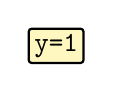
\begin{tikzpicture}[baseline=(ybox.base)]
				\node[
				draw=black,
				line width=0.8pt,
				fill=brightyellow,
				text=black,
				rectangle,
				rounded corners=1pt,
				inner sep=2pt
				] (ybox) {\texttt{y=1}};
			\end{tikzpicture}\\[-2.5pt]
			\begin{minipage}{0.8cm}
				\begin{lstlisting}[language=CustomPseudoCode,numbers=none,basicstyle=\tiny\ttfamily]
// end
				\end{lstlisting}
			\end{minipage}
		};
		
		%––– Response "1" –––
		\node[
		right=0.6cm of state2,
		draw=black,
		line width=0.8pt,
		fill=RedViolet!20,
		text=black,
		diamond,
		aspect=2,
		inner sep=2pt,
		scale=0.7,
		font=\Large
		] (resp1) {\texttt{1}};
		
		%––– Arrows –––
		\draw[->] (main) -- (state1);
		
		% Single transition label: X=0 -> X=1
		\draw[->] (state1) -- node[above] {%
			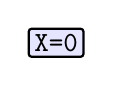
\begin{tikzpicture}[baseline=(a.base)]
				\node[draw=black,line width=0.8pt,fill=blue!10,rectangle,rounded corners=1pt,inner sep=2pt] (a) {\texttt{X=0}};
			\end{tikzpicture}
			$\to$
			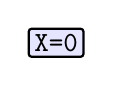
\begin{tikzpicture}[baseline=(b.base)]
				\node[draw=black,line width=0.8pt,fill=blue!10,rectangle,rounded corners=1pt,inner sep=2pt] (b) {\texttt{X=0}};
			\end{tikzpicture}
		} (state2);
		
		% To response "1"
		\draw[->] (state2) -- (resp1);
		
	\end{tikzpicture}
	
	\caption{Network System for interleaving executions of the program in Listing~\ref{lst:MotivatingExample1Ser}.}
\label{fig:code1ExampleNS}
\end{figure}



%\begin{figure}[!htbp]
%	\centering
%	\includegraphics[width=0.9\textwidth]{plots/code_1_NS.png}
%	\caption{Network System for interleaving executions of the program in Listing~\ref{lst:MotivatingExample1Ser}.}
%	\label{fig:code1ExampleNS}
%\end{figure}


%\begin{figure}[!htbp]
%	\centering
%	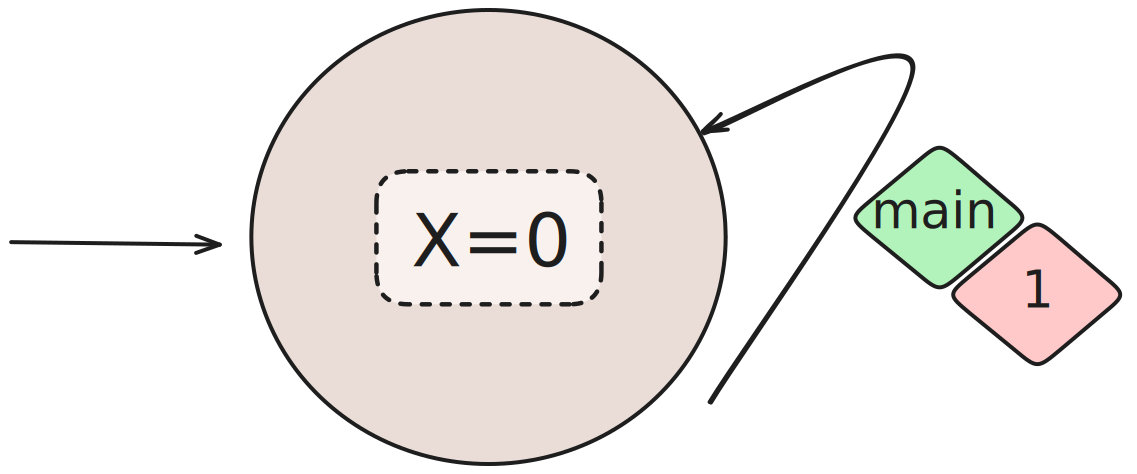
\includegraphics[width=0.35\textwidth]{plots/code_1_NFA.png}
%	\caption{NFA for serial executions of the program in Listing~\ref{lst:MotivatingExample1Ser}.}
%	\label{fig:code1ExampleNFA}
%\end{figure}


\begin{figure}  [!htbp]
	\centering
	% \includegraphics[width=0.48\textwidth,trim=0 0 0 0,clip]{plots/code_single_X0_NFA.pdf}
	
	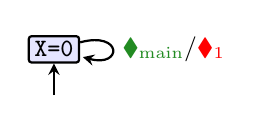
\begin{tikzpicture}[
		->,>=stealth,
		thick,
		node distance=2.5cm,
		state/.style={
			draw=black,
			line width=0.8pt,
			fill=blue!10,
			rectangle,
			rounded corners=1pt,
			inner sep=2pt,
			font=\small
		},
		every node/.style={font=\small}
		]
		% Single state
		\node[state] (X0) {\texttt{X=0}};
		
		% Initial state arrow
		\draw[->] ([yshift=-0.4cm]X0.south) -- (X0.south);
		
		% Self-loop with main/1 using the paper's colored lozenge notation
		\draw[->] (X0) edge[loop right]
		node[right] {${\color{ForestGreen}\blacklozenge_{\mathrm{main}}}/{\color{red}\blacklozenge_1}$} (X0);
	\end{tikzpicture}
	
	\caption{NFA for serial executions of the program in Listing~\ref{lst:MotivatingExample1Ser}.}
\label{fig:code1ExampleNFA}
\end{figure}




\begin{figure}[H]
	\centering
	\includegraphics[width=0.6\textwidth]{plots/code_1_PN_with_annotation.png}
	\caption{Petri net for interleaving executions of the program in Listing~\ref{lst:MotivatingExample1Ser}.}
	\label{fig:code1ExamplePN}
\end{figure}


%

\subsection{Translation Example: Listing~\ref{lst:MotivatingExample2NonSer}}
\label{appendix:subsec::Ex1B:NS}

The Network System, Serializability NFA, and Pet net of Listing~\ref{lst:MotivatingExample2NonSer} are depicted in the main text (see subsec.~\ref{subsec:SerToNsTranslation}).
%
We present in Fig.~\ref{fig:code2ExampleNSSecondPart} the mappings \(\delta\), $req$, and $resp$.

\begin{figure}[!htbp]
	\centering
	%–––– Network system diagram ––––
	% \includegraphics[width=\textwidth]{plots/code_2_NS.png}\\[1ex]
	
	%–––– req, resp, and δ definitions ––––
	\[
	\begin{array}{@{}r@{\;}l}
		req \coloneq & 
		\big\{
		\big[
		\begin{array}{c c c}
			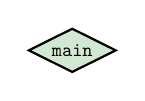
\begin{tikzpicture}[baseline=(textnode.base)]
				\node[
				draw=black,
				line width=0.8pt,
				fill=ForestGreen!20,
				text=black,
				diamond,
				aspect=2,
				inner sep=2pt,
				scale=0.7
				] (textnode) {\texttt{main}};
			\end{tikzpicture}
			&\!\!\rightarrow\!\!&
			\begin{array}{c}
				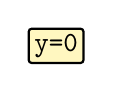
\begin{tikzpicture}[baseline=(ybox.base)]
					\node[
					draw=black,
					line width=0.8pt,
					fill=brightyellow,
					text=black,
					rectangle,
					rounded corners=1pt,
					inner sep=2pt
					] (ybox) {\texttt{y=0}};
				\end{tikzpicture}\vspace{-2pt}
				\\
				\begin{minipage}{0.20\linewidth}
					\begin{lstlisting}[language=CustomPseudoCode,numbers=none,basicstyle=\tiny\ttfamily]
X := 1 
yield 
y := X
X := 0
return y
					\end{lstlisting}
				\end{minipage}
			\end{array}
		\end{array}
		\big]
		\big\}
		\\[2em]
		resp \coloneq &
		\big\{
		\big[
		\begin{array}{c c c}
			\begin{array}{c}
				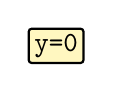
\begin{tikzpicture}[baseline=(ybox.base)]
					\node[
					draw=black,
					line width=0.8pt,
					fill=brightyellow,
					text=black,
					rectangle,
					rounded corners=1pt,
					inner sep=2pt
					] (ybox) {\texttt{y=0}};
				\end{tikzpicture}\vspace{-2pt}
				\\
				\begin{minipage}{0.11\linewidth}
					\begin{lstlisting}[language=CustomPseudoCode,numbers=none,basicstyle=\tiny\ttfamily]
// end
					\end{lstlisting}
				\end{minipage}
			\end{array}
			&\!\!\rightarrow\!\!&
			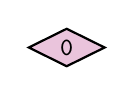
\begin{tikzpicture}[baseline=(textnode.base),scale=0.7]
				\node[
				draw=black,
				line width=0.8pt,
				fill=RedViolet!20,
				text=black,
				diamond,
				aspect=2,
				inner sep=2pt,
				font=\small
				] (textnode) {\texttt{0}};
			\end{tikzpicture}
		\end{array}
		\big]\,{},
		\big[
		\begin{array}{c c c}
			\begin{array}{c}
				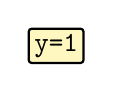
\begin{tikzpicture}[baseline=(ybox.base)]
					\node[
					draw=black,
					line width=0.8pt,
					fill=brightyellow,
					text=black,
					rectangle,
					rounded corners=1pt,
					inner sep=2pt
					] (ybox) {\texttt{y=1}};
				\end{tikzpicture}\vspace{-2pt}
				\\
				\begin{minipage}{0.11\linewidth}
					\begin{lstlisting}[language=CustomPseudoCode,numbers=none,basicstyle=\tiny\ttfamily]
// end
					\end{lstlisting}
				\end{minipage}
			\end{array}
			&\!\!\rightarrow\!\!&
			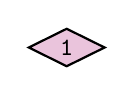
\begin{tikzpicture}[baseline=(textnode.base),scale=0.7]
				\node[
				draw=black,
				line width=0.8pt,
				fill=RedViolet!20,
				text=black,
				diamond,
				aspect=2,
				inner sep=2pt,
				font=\small
				] (textnode) {\texttt{1}};
			\end{tikzpicture}
		\end{array}
		\big]
		\big\}
		\\[2em]
		\delta \coloneq & 
		\big\{\big[(
		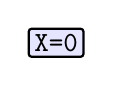
\begin{tikzpicture}[baseline=(ybox.base)]
			\node[
			draw=black,
			line width=0.8pt,
			fill=blue!10,
			text=black,
			rectangle,
			rounded corners=1pt,
			inner sep=2pt
			] (ybox) {\texttt{X=0}};
		\end{tikzpicture}\,{},
		\begin{array}{c}
			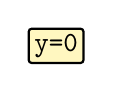
\begin{tikzpicture}[baseline=(ybox.base)]
				\node[
				draw=black,
				line width=0.8pt,
				fill=brightyellow,
				text=black,
				rectangle,
				rounded corners=1pt,
				inner sep=2pt
				] (ybox) {\texttt{y=0}};
			\end{tikzpicture}\vspace{-2pt}
			\\
			\begin{minipage}{0.14\linewidth}
				\begin{lstlisting}[language=CustomPseudoCode,numbers=none,basicstyle=\tiny\ttfamily]
X := 1
yield
y := X
X := 0
return y
				\end{lstlisting}
			\end{minipage}
		\end{array}
		)
		\;\rightarrow\;
		(
		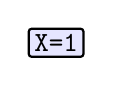
\begin{tikzpicture}[baseline=(ybox.base)]
			\node[
			draw=black,
			line width=0.8pt,
			fill=blue!10,
			text=black,
			rectangle,
			rounded corners=1pt,
			inner sep=2pt
			] (ybox) {\texttt{X=1}};
		\end{tikzpicture}\,{},
		\begin{array}{c}
			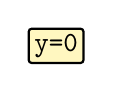
\begin{tikzpicture}[baseline=(ybox.base)]
				\node[
				draw=black,
				line width=0.8pt,
				fill=brightyellow,
				text=black,
				rectangle,
				rounded corners=1pt,
				inner sep=2pt
				] (ybox) {\texttt{y=0}};
			\end{tikzpicture}\vspace{-2pt}
			\\
			\begin{minipage}{0.14\linewidth}
				\begin{lstlisting}[language=CustomPseudoCode,numbers=none,basicstyle=\tiny\ttfamily]
y := X
X := 0
return y
				\end{lstlisting}
			\end{minipage}
		\end{array}
		)
		\big],
		\\[0.5em]
		& \phantom{\big\{}
		\big[(
		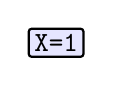
\begin{tikzpicture}[baseline=(ybox.base)]
			\node[
			draw=black,
			line width=0.8pt,
			fill=blue!10,
			text=black,
			rectangle,
			rounded corners=1pt,
			inner sep=2pt
			] (ybox) {\texttt{X=1}};
		\end{tikzpicture}\,{},
		\begin{array}{c}
			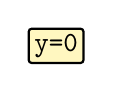
\begin{tikzpicture}[baseline=(ybox.base)]
				\node[
				draw=black,
				line width=0.8pt,
				fill=brightyellow,
				text=black,
				rectangle,
				rounded corners=1pt,
				inner sep=2pt
				] (ybox) {\texttt{y=0}};
			\end{tikzpicture}\vspace{-2pt}
			\\
			\begin{minipage}{0.14\linewidth}
				\begin{lstlisting}[language=CustomPseudoCode,numbers=none,basicstyle=\tiny\ttfamily]
y := X
X := 0
return y
				\end{lstlisting}
			\end{minipage}
		\end{array}
		)
		\;\rightarrow\;
		(
		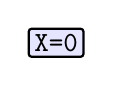
\begin{tikzpicture}[baseline=(ybox.base)]
			\node[
			draw=black,
			line width=0.8pt,
			fill=blue!10,
			text=black,
			rectangle,
			rounded corners=1pt,
			inner sep=2pt
			] (ybox) {\texttt{X=0}};
		\end{tikzpicture}\,{},
		\begin{array}{c}
			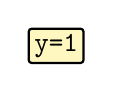
\begin{tikzpicture}[baseline=(ybox.base)]
				\node[
				draw=black,
				line width=0.8pt,
				fill=brightyellow,
				text=black,
				rectangle,
				rounded corners=1pt,
				inner sep=2pt
				] (ybox) {\texttt{y=1}};
			\end{tikzpicture}
			\vspace{-2pt}
			\\
			\begin{minipage}{0.11\linewidth}
				\begin{lstlisting}[language=CustomPseudoCode,numbers=none,basicstyle=\tiny\ttfamily]
// end
				\end{lstlisting}
			\end{minipage}
		\end{array}
		)
		\big],
		\ldots
		\big\}
	\end{array}
	\]
	\caption{The \(\delta\) transition function, and the \(req\) and \(resp\) mappings for the program in Listing~\ref{lst:MotivatingExample2NonSer}.}
	\label{fig:code2ExampleNSSecondPart}
\end{figure}



\subsection{Translation Example: Listing~\ref{lst:MotivatingExample3Ser}}
\label{appendix:subsec:Ex1C:NS}


For our third motivating example, presented in Listing~\ref{lst:MotivatingExample3Ser}, we denote the Network System in Fig.~\ref{fig:code3ExampleNS}, the Serializability NFA in Fig.~\ref{fig:code3ExampleNFA}, and the Interleaving Petri net in Fig.~\ref{fig:code3ExamplePN}.

%\begin{minipage}[t]{0.3\textwidth}
%	\begin{lstlisting}[caption={With yield and lock (serializable)}]
%		request foo: 
%			// lock
%			while (L == 1): 
%				yield
%			L := 1 
%		
%			X := 1
%			yield
%			y := X 
%			X := 0
%		
%			// unlock    
%			L := 0
%			return y 
%	\end{lstlisting}
%\end{minipage}
%
%This program corresponds to the following Network System (NS):

%\begin{figure}[!htbp]
%	\centering
%	\includegraphics[width=1.1\textwidth]{plots/code_3_NS.png}
%	\caption{Network System for interleaving executions of the program in Listing~\ref{lst:MotivatingExample3Ser}.}
%	\label{fig:code3ExampleNS}
%\end{figure}


\begin{figure}[!htbp]
	\centering
	% \includegraphics[width=\textwidth]{plots/code_locking_NS.png}\\[1ex]
	
	\begin{tikzpicture}[
		node distance=1.5cm and 2.5cm,
		>=stealth,
		thick,
		every node/.style={font=\small}
		]
		%–––– Request (green diamond) ––––
		\node[
		draw=black,
		line width=0.8pt,
		fill=ForestGreen!20,
		text=black,
		diamond,
		aspect=2,
		inner sep=2pt,
		scale=0.7
		] (main) {\texttt{main}};
		
		%–––– State 1: y=0 + locked program ––––
		\node[right=0.7cm of main, align=center] (state1) {
			\begin{tikzpicture}[baseline=(ybox.base)]
				\node[
				draw=black,
				line width=0.8pt,
				fill=brightyellow,
				text=black,
				rectangle,
				rounded corners=1pt,
				inner sep=2pt
				] (ybox) {\texttt{y=0}};
			\end{tikzpicture}\\[-2.5pt]
			\begin{minipage}{2.6cm}
				\begin{lstlisting}[language=CustomPseudoCode,numbers=none,basicstyle=\tiny\ttfamily]
while (L == 1):
	yield
L := 1

X := 1
yield
y := X
X := 0

// unlock
L := 0
return y
				\end{lstlisting}
			\end{minipage}
		};
		
		%–––– State 2: y=0 + tail program ––––
		\node[right=of state1, xshift=12mm, align=center] (state2) {
			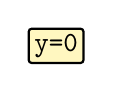
\begin{tikzpicture}[baseline=(ybox.base)]
				\node[
				draw=black,
				line width=0.8pt,
				fill=brightyellow,
				text=black,
				rectangle,
				rounded corners=1pt,
				inner sep=2pt
				] (ybox) {\texttt{y=0}};
			\end{tikzpicture}\\[-2.5pt]
			\begin{minipage}{2.0cm}
				\begin{lstlisting}[language=CustomPseudoCode,numbers=none,basicstyle=\tiny\ttfamily]
y := X
X := 0

// unlock
L := 0
return y
				\end{lstlisting}
			\end{minipage}
		};
		
		%–––– State 3 (top-right): //end, y=0 ––––
		\node[above right=-0.5cm and 2.2cm of state2, align=center] (state3) {
			\begin{tikzpicture}[baseline=(ybox.base)]
				\node[
				draw=black,
				line width=0.8pt,
				fill=brightyellow,
				text=black,
				rectangle,
				rounded corners=1pt,
				inner sep=2pt
				] (ybox) {\texttt{y=0}};
			\end{tikzpicture}\\[-2.5pt]
			\begin{minipage}{0.9cm}
				\begin{lstlisting}[language=CustomPseudoCode,numbers=none,basicstyle=\tiny\ttfamily]
// end
				\end{lstlisting}
			\end{minipage}
		};
		
		%–––– State 4 (bottom-right): //end, y=1 ––––
		\node[below right=-0.2cm and 2.2cm of state2, align=center] (state4) {
			\begin{tikzpicture}[baseline=(ybox.base)]
				\node[
				draw=black,
				line width=0.8pt,
				fill=brightyellow,
				text=black,
				rectangle,
				rounded corners=1pt,
				inner sep=2pt
				] (ybox) {\texttt{y=1}};
			\end{tikzpicture}\\[-2.5pt]
			\begin{minipage}{0.9cm}
				\begin{lstlisting}[language=CustomPseudoCode,numbers=none,basicstyle=\tiny\ttfamily]
// end
				\end{lstlisting}
			\end{minipage}
		};
		
		%–––– Responses ––––
		\node[
		right=0.6cm of state3,
		draw=black,
		line width=0.8pt,
		fill=RedViolet!20,
		text=black,
		diamond,
		aspect=2,
		inner sep=2pt,
		scale=0.7,
		font=\Large
		] (resp0) {\texttt{0}};
		
		\node[
		right=0.6cm of state4,
		draw=black,
		line width=0.8pt,
		fill=RedViolet!20,
		text=black,
		diamond,
		aspect=2,
		inner sep=2pt,
		scale=0.7,
		font=\Large
		] (resp1) {\texttt{1}};
		
		%–––– Arrows ––––
		\draw[->] (main) -- (state1);
		
		% Self-loop on state1: (X=1,L=1) -> (X=1,L=1)
		\draw[->] (state1) edge[loop above]
		node[above] {%
			\begin{tikzpicture}[baseline=(a.base)]
				\node[draw=black,line width=0.8pt,fill=blue!10,rectangle,rounded corners=1pt,inner sep=2pt] (a) {\texttt{X=1, L=1}};
			\end{tikzpicture}
			$\to$
			\begin{tikzpicture}[baseline=(b.base)]
				\node[draw=black,line width=0.8pt,fill=blue!10,rectangle,rounded corners=1pt,inner sep=2pt] (b) {\texttt{X=1, L=1}};
			\end{tikzpicture}
		} (state1);
		
		% Transition state1 -> state2: (X=0,L=0) -> (X=1,L=1)
		\draw[->] (state1) -- node[above] {%
			\begin{tikzpicture}[baseline=(a.base)]
				\node[draw=black,line width=0.8pt,fill=blue!10,rectangle,rounded corners=1pt,inner sep=2pt] (a) {\texttt{X=0, L=0}};
			\end{tikzpicture}
			$\to$
			\begin{tikzpicture}[baseline=(b.base)]
				\node[draw=black,line width=0.8pt,fill=blue!10,rectangle,rounded corners=1pt,inner sep=2pt] (b) {\texttt{X=1, L=1}};
			\end{tikzpicture}
		} (state2);
		
		% Transition state2 -> state3: (X=0,L=0) -> (X=0,L=0)
		\draw[->] ([yshift=4pt]state2.east) to[out=50,in=180]
		node[above,sloped] {%
			\begin{tikzpicture}[baseline=(a.base)]
				\node[draw=black,line width=0.8pt,fill=blue!10,rectangle,rounded corners=1pt,inner sep=2pt] (a) {\texttt{X=0, L=0}};
			\end{tikzpicture}
			$\to$
			\begin{tikzpicture}[baseline=(b.base)]
				\node[draw=black,line width=0.8pt,fill=blue!10,rectangle,rounded corners=1pt,inner sep=2pt] (b) {\texttt{X=0, L=0}};
			\end{tikzpicture}
		} (state3.west);
		
		% Transition state2 -> state4: (X=1,L=1) -> (X=0,L=0)
		\draw[->] ([yshift=-16pt]state2.east) to[out=-50,in=180]
		node[below,sloped] {%
			\begin{tikzpicture}[baseline=(a.base)]
				\node[draw=black,line width=0.8pt,fill=blue!10,rectangle,rounded corners=1pt,inner sep=2pt] (a) {\texttt{X=1, L=1}};
			\end{tikzpicture}
			$\to$
			\begin{tikzpicture}[baseline=(b.base)]
				\node[draw=black,line width=0.8pt,fill=blue!10,rectangle,rounded corners=1pt,inner sep=2pt] (b) {\texttt{X=0, L=0}};
			\end{tikzpicture}
		} (state4.west);
		
		% To responses
		\draw[->] (state3) -- (resp0);
		\draw[->] (state4) -- (resp1);
		
	\end{tikzpicture}
	
	\caption{Network System for interleaving executions of the program in Listing~\ref{lst:MotivatingExample3Ser}.}
\label{fig:code3ExampleNS}
\end{figure}



%\begin{figure}[!htbp]
%	\centering
%	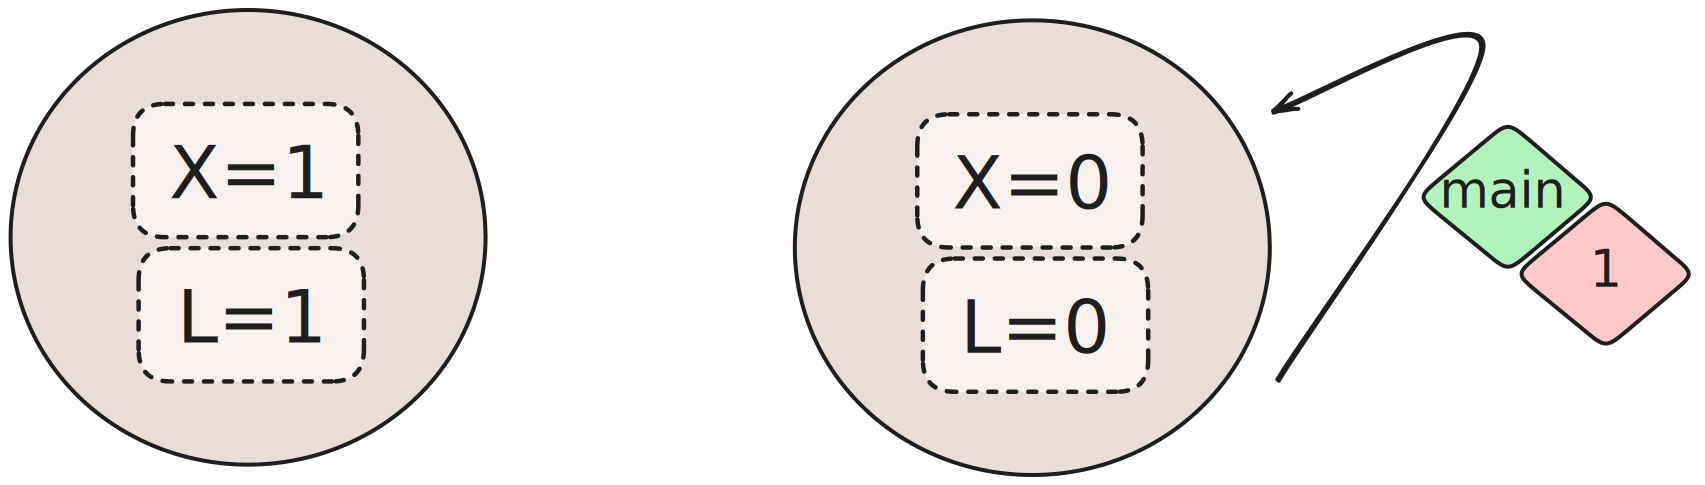
\includegraphics[width=0.4\textwidth]{plots/code_3_NFA.png}
%	\caption{NFA for serial executions of the program in Listing~\ref{lst:MotivatingExample3Ser}.}
%	\label{fig:code3ExampleNFA}
%\end{figure}


\begin{figure}  [!htbp]
	\centering
	% \includegraphics[width=0.48\textwidth,trim=0 0 0 0,clip]{plots/code_two_states_XL_NFA.pdf}
	
	\begin{tikzpicture}[
		->,>=stealth,
		thick,
		node distance=2.5cm,
		state/.style={
			draw=black,
			line width=0.8pt,
			fill=blue!10,
			rectangle,
			rounded corners=1pt,
			inner sep=2pt,
			font=\small
		},
		every node/.style={font=\small}
		]
		% States
		\node[state] (X1L1) {\texttt{X=1, L=1}};
		\node[state, right of=X1L1] (X0L0) {\texttt{X=0, L=0}};
		
		% No edges to or from X=1, L=1 (isolated)
		
		% Self-loop on X=0, L=0 with main/1 (colored lozenge notation)
		\draw[->] (X0L0) edge[loop right]
		node[right] {${\color{ForestGreen}\blacklozenge_{\mathrm{main}}}/{\color{red}\blacklozenge_1}$} (X0L0);
	\end{tikzpicture}
	
	\caption{NFA for serial executions of the program in Listing~\ref{lst:MotivatingExample3Ser}.}
\label{fig:code3ExampleNFA}
\end{figure}




\begin{figure}[!htbp]
	\centering
	\includegraphics[width=0.8\textwidth]{plots/code_3_PN_with_annotation.png}
	\caption{Petri net for interleaving executions of the program in Listing~\ref{lst:MotivatingExample3Ser}.}
	\label{fig:code3ExamplePN}
\end{figure}

%\newpage
	\clearpage

\section{Translating Network Systems to Petri Nets}
\label{appendix:NS-to-PN-formulation}


We denote with \(\mathbf0\) a zero vector of dimension \(|P|\), and with \(\mathbf1_{p}\) a \(|P|\)-sized indicator vector that has 0 in every coordinate except the one corresponding to place \(p \in P\), which has 1. 
% 
The flow functions $\mathsf{pre},\mathsf{post}:T\to\{0,1\}^{|P|}$ assign to each transition $t$ a binary vector over $P$ whose $1$-entries mark the places from which tokens are consumed (for $\mathsf{pre}(t)$) and to which tokens are produced (for $\mathsf{post}(t)$) when $t$ fires.
A transition $t$ is enabled at $M$ iff $\mathsf{pre}(t)\le M$ (component-wise); firing yields
\(
M\xrightarrow{t}M' \quad\text{where}\quad M' = M-\mathsf{pre}(t)+\mathsf{post}(t)
\).	

\medskip
\textit{Construction.}
We generate the Petri net:
\[
N_{\mathrm{int}}(\mathcal S)
= (P,\,T,\,\mathsf{pre},\,\mathsf{post},\,M_0),
\]
where
\[
P
=
P_G \;\cup\; P_{REQ,L} \;\cup\; P_{REQ,RESP}
\]

for 
\[
\begin{aligned}
	P_G
	&= \{\,p_g \mid g\in G\},\quad
	P_{REQ,L}
	= \bigl\{\,p_{({\color{ForestGreen}\blacklozenge_{\mathit{req}}},\ell)}
	\mid {\color{ForestGreen}\blacklozenge_{\mathit{req}}}\in\mathit{REQ},\,\ell\in  L\bigr\},\\[1ex]
	P_{REQ,RESP}
	&= \bigl\{\,p_{({\color{ForestGreen}\blacklozenge_{\mathit{req}}}/{\color{red}\blacklozenge_{\mathit{resp}}})}
	\mid {\color{ForestGreen}\blacklozenge_{\mathit{req}}}\in\mathit{REQ},\,
	{\color{red}\blacklozenge_{\mathit{resp}}}\in\mathit{RESP}\bigr\}.
\end{aligned}
\]


%	\[
%	\begin{aligned}
	%		P_G &= \{\,p_g \mid g\in G\},\;\,
	%		P_{REQ,L} = \{\,p_{{\color{ForestGreen}\blacklozenge_{\mathit{req}}}/\ell}
	%		\mid {\color{ForestGreen}\blacklozenge_{\mathit{req}}}\in\mathit{REQ},\,\ell\in L\},\\
	%		P_{REQ,RESP} &= \{\,p_{{\color{ForestGreen}\blacklozenge_{\mathit{req}}}/{\color{red}\blacklozenge_{\mathit{resp}}}}
	%		\mid {\color{ForestGreen}\blacklozenge_{\mathit{req}}}\in\mathit{REQ},\,
	%		{\color{red}\blacklozenge_{\mathit{resp}}}\in\mathit{RESP}\}.
	%	\end{aligned}
%	\]

%	\[
%	P_G 
%	= \{\,p_g \mid g\in G\}
%	\quad 
%%	P_L 
%%	= \{\,p_\ell \mid \ell\in L\}
%%	\quad
%	P_{REQ,L} =
%	\{\,p_{{\color{ForestGreen}\blacklozenge_{\mathit{req}}}/\ell} \mid
%	{\color{ForestGreen}\blacklozenge_{\mathit{req}}}\in \mathit{REQ}, \ell\in L\},%\\
%	\quad
%	P_{REQ,RESP}=
%	\{\,p_{{\color{ForestGreen}\blacklozenge_{\mathit{req}}}/{\color{red}\blacklozenge_{\mathit{resp}}}} \mid
%	{\color{ForestGreen}\blacklozenge_{\mathit{req}}}\in \mathit{REQ}, {\color{red}\blacklozenge_{\mathit{resp}}}\in \mathit{RESP}\},
%	\]
%	\{\,p_{{\color{ForestGreen}\blacklozenge_{\mathit{req}}}/{\color{red}\blacklozenge_{\mathit{resp}}}} \mid
%	{\color{ForestGreen}\blacklozenge_{\mathit{req}}}\in \mathit{REQ}, {\color{red}\blacklozenge_{\mathit{resp}}}\in \mathit{RESP}\},
%	\]

%	\[
%	P_{REQ,RESP}=
%	\{\,p_{{\color{ForestGreen}\blacklozenge_{\mathit{req}}}/{\color{red}\blacklozenge_{\mathit{resp}}}} \mid
%	{\color{ForestGreen}\blacklozenge_{\mathit{req}}}\in \mathit{REQ}, {\color{red}\blacklozenge_{\mathit{resp}}}\in \mathit{RESP}\},
%	\]

with \(G\) being the set of global states, \(L\) being the set of local states (in the case of a \toolname-derived NS, this is the coupling of the local variable assignments of an in-flight request and its remaining \toolname{} program to execute), \(\mathit{REQ}\) denotes the request labels; and \(\mathit{RESP}\) denotes the response labels.

\medskip
Transitions are partitioned as:
\[
T = T_{\mathit{req}} \;\cup\; T_{\delta}\;\cup\;T_{\mathit{resp}}
\]
where

%	\[
%	T_{\mathit{req}} = \{\,t_{({\color{ForestGreen}\blacklozenge_{\mathit{req}}},\ell)} \mid {(\color{ForestGreen}\blacklozenge_{\mathit{req}}},\ell)\in\mathit{req}\},\quad
%	T_{\delta} = \{\,t_{(\ell,g)\to(\ell',g')} \mid (\ell,g)\xrightarrow{}(\ell',g')\in\delta\},\quad
%	T_{\mathit{resp}} = \{\,t_{(\ell,{\color{red}\blacklozenge_{\mathit{resp}}})} \mid (\ell,{\color{red}\blacklozenge_{\mathit{resp}}})\in\mathit{resp}\}.
%	\]

\begin{align*}
	T_{\mathit{req}}
	&= \{\,t_{({\color{ForestGreen}\blacklozenge_{\mathit{req}}},\ell)} \mid {(\color{ForestGreen}\blacklozenge_{\mathit{req}}},\ell)\in\mathit{req}\},\\[1ex]
	T_{\delta}
	&= \bigl\{\,t_{((\ell,g),(\ell',g'))} 
	\mid ((\ell,g),(\ell',g'))\in\delta\bigr\},\quad
	T_{\mathit{resp}}
	= \{\,t_{(\ell,{\color{red}\blacklozenge_{\mathit{resp}}})} \mid (\ell,{\color{red}\blacklozenge_{\mathit{resp}}})\in\mathit{resp}\}.
\end{align*}



%\smallskip
%Given a local state \(\ell\) which resulted from a request \({\color{ForestGreen}\blacklozenge_{\mathit{req}}}\) (either directly or downstream due to program execution) --- the transitions are:
Their \(\mathsf{pre}\) and \(\mathsf{post}\) flow functions are:
\[
\begin{alignedat}{3}
	\mathsf{pre}\bigl(t_{({\color{ForestGreen}\blacklozenge_{\mathit{req}}},\ell)}\bigr)
	&= \mathbf0, &
	\mathsf{post}\bigl(t_{({\color{ForestGreen}\blacklozenge_{\mathit{req}}},\ell)}\bigr)
	&= \mathbf1_{p_{({\color{ForestGreen}\blacklozenge_{\mathit{req}}},\ell)}}, 
	&&\text{for }({\color{ForestGreen}\blacklozenge_{\mathit{req}}},\ell)\in\mathit{req},\\
	\mathsf{pre}\bigl(t_{((\ell,g),(\ell',g'))}\bigr)
	&= \mathbf1_{p_{({\color{ForestGreen}\blacklozenge_{\mathit{req}}},\ell)}} + \mathbf1_{p_g}, &
	\mathsf{post}\bigl(t_{((\ell,g),(\ell',g'))}\bigr)
	&= \mathbf1_{p_{({\color{ForestGreen}\blacklozenge_{\mathit{req}}},\ell')}} + \mathbf1_{p_{g'}}, 
	&&\text{for }{{\color{ForestGreen}\blacklozenge_{\mathit{req}}}\in\mathit{REQ}}, ((\ell,g),(\ell',g'))\in\delta,\\
	\mathsf{pre}\bigl(t_{(\ell,{\color{red}\blacklozenge_{\mathit{resp}}})}\bigr)
	&= \mathbf1_{p_{({\color{ForestGreen}\blacklozenge_{\mathit{req}}},\ell)}}, &
	\mathsf{post}\bigl(t_{(\ell,{\color{red}\blacklozenge_{\mathit{resp}}})}\bigr)
	&= \mathbf1_{p_{({\color{ForestGreen}\blacklozenge_{\mathit{req}}}/{\color{red}\blacklozenge_{\mathit{resp}}})}}, 
	&&\text{for }{{\color{ForestGreen}\blacklozenge_{\mathit{req}}}\in\mathit{REQ},(\ell,\color{red}\blacklozenge_{\mathit{resp}}})\in\mathit{resp}
	%\ %(\ell\text{ the matching local state).
		%		}
\end{alignedat}
\]

Where for the last two cases, \({\color{ForestGreen}\blacklozenge_{\mathit{req}}}\) concerns requests that eventually give rise to a local state \(\ell \in L\) that originated downstream (during execution).

\medskip
The initial marking is a single token on the single place representing the initial global state $g_0$ of the NS:
\[
M_0(p_{g_0}) = 1,
\quad
M_0(p) = 0 \text{ for all }p\neq p_{g_0},
\]
%	where \(g_0\) is the initial global state of the network system \(\mathcal S\).  



Define the projection \(\pi\) to solely include the markings of places representing completed request/response pairs.
% (with the exception of a single token on a state in \(P_G\)).
%\[
%\pi \;:\;\mathbb N^P \;\longrightarrow\;\mathbb N^{P_R}
%\quad\bigl(\pi(M)\bigr)(p_{({{\color{ForestGreen}\blacklozenge_{\mathit{req}}}/{\color{red}\blacklozenge_{\mathit{resp}}}})})\;=\;M(p_{({{\color{ForestGreen}\blacklozenge_{\mathit{req}}}/{\color{red}\blacklozenge_{\mathit{resp}}}})})\text{ for }p_{({{\color{ForestGreen}\blacklozenge_{\mathit{req}}}/{\color{red}\blacklozenge_{\mathit{resp}}}})}\in P_{REQ,RESP}.
%\]
Then, the multiset of all  (${{\color{ForestGreen}\blacklozenge_{\mathit{req}}}/{\color{red}\blacklozenge_{\mathit{resp}}}}$) pairs of the NS, obtained by \textit{any} interleaving, is:
\[
\mathsf{Int}(\mathcal S)
\;=\;
\bigl\{\;\pi(M)\;\bigm|\;M_0 \xrightarrow{}^{*} M\text{ in }N_{\mathrm{int}}(\mathcal S)\bigr\}.
\]
	
\section{Example: Serializable Program}
\label{appendix:ns-serializable}


Now, we observe again the adjusted program with a spin-lock (as previously described in Listing~\ref{lst:MotivatingExample3Ser}), of which we depicted figures of the corresponding Network System (Fig.~\ref{fig:code3ExampleNS}), Serializability NFA (Fig.~\ref{fig:code3ExampleNFA}), and the interleaving Petri net (Fig.~\ref{fig:code3ExamplePN}) in Appendix~\ref{appendix:MoreNsExamples}.
%
In this case, serializability corresponds to the Petri net being unable to reach a marking satisfying the same semilinear formula \(\mathcal {F}\) as in the non-serializable case described in the main text (subsec.~\ref{subsec:SerToNsTranslation}):

\[
\mathcal {F}:
\quad
P_1 = 0 \wedge 
\textcolor{blue}{P_2} \ge 0 \wedge \textcolor{blue}{P_3} \ge 0  \wedge P_4 = 0
\wedge P_5 = 0 \wedge P_6 = 0 \wedge \textcolor{red}{P_7} \ge 0 \wedge \textcolor{red}{P_8} \ge 1.
\]

% (note however, that this is not always the case). 
%(but this time each place $P_i$ corresponds to the new PN). 
%following formula:
%
%\[
%\textcolor{blue}
%P_1 = 0 \wedge 
%{P_2} \ge 0 \wedge \textcolor{blue}{P_3} \ge 0  \wedge P_4 = 0
%\wedge P_5 = 0 \wedge P_6 = 0 \wedge \textcolor{red}{P_7} = 0 \wedge \textcolor{red}{P_8} \ge 1.
%\]


In addition, although the target set is the same as in the previous example, the Petri net places $(P_1,\ldots,P_8)$ encode different states that correspond to the updated network system. For instance, now each place in the PN that encodes a global state accounts for two global variables, \texttt{X} and \texttt{L}, and the initial global state corresponds to the place encoding the initial assignment \textcolor{blue}{[X=0, L=0]}, etc.
%
Furthermore, unlike the case in Listing~\ref{lst:MotivatingExample2NonSer} (covered in subsec.~\ref{subsec:SerToNsTranslation}), this target set of markings (encoding request/response pairs of non-serial executions) is \textit{unreachable}, as witnessed by the inductive invariant:


\[
\begin{aligned}
	&(P_{1},\textcolor{blue}{P_{2}},\textcolor{blue}{P_{3}},P_{4},P_{5},P_{6},\textcolor{red}{P_{7}},\textcolor{red}{P_{8}})
	\;\mapsto\;\\
	&\quad
	\exists\,e_{0},\dots,e_{5}\ge0.\;
	\Bigl(
	e_{2}-e_{1}+\textcolor{blue}{P_{3}}-1=0\;\land\;
	e_{2}+P_{1}-e_{5}=0\;\land\;
	P_{5}-e_{1}+e_{4}=0\;\land\\
	&\qquad\quad
	-\,e_{4}+\textcolor{red}{P_{7}}=0\;\land\;
	P_{6}+e_{3}-e_{0}=0\;\land\;
	\textcolor{red}{P_{8}}-e_{3}=0\;\land\\
	&\qquad\quad
	-\,e_{2}+e_{1}+e_{0}+P_{4}=0\;\land\;
	-\,e_{2}+e_{1}+\textcolor{blue}{P_{2}}=0
	\Bigr)
	\;\land\;
	\bigl(P_{4}-1\ge0\;\lor\;\textcolor{blue}{P_{3}}-1\ge0\bigr).
\end{aligned}
\]


We then revert and project it on the request/response pairs of the network system.
%
We get the following inductive invariants for each of the two (reachable) global states:

\begin{proof}
	
	\medskip\noindent
	For global state \textcolor{blue}{[L=0,X=0]} the projected invariant is:
	\[
	\bigl(\,\text{\color{ForestGreen}$\blacklozenge_{\text{main}}$}/\text{\color{red}$\blacklozenge_{0}$},\;
	\text{\color{ForestGreen}$\blacklozenge_{\text{main}}$}/\text{\color{red}$\blacklozenge_{1}$}\bigr)
	\;\mapsto\;
	\exists\,e_{0},\dots,e_{5}\ge0.\;
	\begin{aligned}[t]
		& e_{2}-e_{1}=0,\quad
		e_{2}-e_{5}=0,\quad
		-e_{1}+e_{4}=0,\\
		& -e_{4}+\bigl(\text{\color{ForestGreen}$\blacklozenge_{\text{main}}$}/\text{\color{red}$\blacklozenge_{1}$}\bigr)=0,\quad
		-e_{0}+e_{3}=0,\\
		& -e_{3}+\bigl(\text{\color{ForestGreen}$\blacklozenge_{\text{main}}$}/\text{\color{red}$\blacklozenge_{0}$}\bigr)=0,\quad
		-e_{2}+e_{1}+e_{0}=0,\\
		& -e_{2}+e_{1}=0.
	\end{aligned}
	\]
	\noindent From 
	\[e_{1}=e_{2}=e_{4}=e_{5}=(\;
	\text{\color{ForestGreen}$\blacklozenge_{\text{main}}$}/\text{\color{red}$\blacklozenge_{1}$}),\;
	e_{0}=e_{3}=
	(\text{\color{ForestGreen}$\blacklozenge_{\text{main}}$}/\text{\color{red}$\blacklozenge_{0}$})
	\]
	
	it follows that \[-e_{2}+e_{1}+e_{0}=0\;\Longrightarrow\;e_{0}=0,\]
	
	thus: 
	\[
	(	\text{\color{ForestGreen}$\blacklozenge_{\text{main}}$}/\text{\color{red}$\blacklozenge_{0}$})
	=0 \quad \text{and} \quad (	\text{\color{ForestGreen}$\blacklozenge_{\text{main}}$}/\text{\color{red}$\blacklozenge_{1}$})
	=0
	\]
	
	indicating that  (\(\text{\color{ForestGreen}$\blacklozenge_{\text{main}}$}/\text{\color{red}$\blacklozenge_{0}$}\)) cannot be obtained from the global state
	\textcolor{blue}{[L=0,X=0]}.
	
	\medskip\noindent
	In the second case, for the global state \textcolor{blue}{[L=1, X=1]}
	the projected invariant is:
	
	
	\[
	\bigl(\,\text{\color{ForestGreen}$\blacklozenge_{\text{main}}$}/\text{\color{red}$\blacklozenge_{0}$},\;
	\text{\color{ForestGreen}$\blacklozenge_{\text{main}}$}/\text{\color{red}$\blacklozenge_{1}$}\bigr)
	\;\mapsto\;
	\exists\,e_{0},\dots,e_{5}.\;\bot,
	\]
	which is unsatisfiable. Hence, no completed request/response pair, and in particular, no (\(\text{\color{ForestGreen}$\blacklozenge_{\text{main}}$}/\text{\color{red}$\blacklozenge_{0}$}\)) pair can be produced from this state via \textit{any} execution. Intuitively, this aligns with the fact that there cannot be any output generated via an interleaving, given that the spin-lock is acquired (\textcolor{blue}{[L=1]}).
	%	\guy{Mark/Jules is this part correct?}
	
	\medskip
	\noindent\textbf{Conclusion.}
	In every reachable state, no request/response pair of the form
	($	\text{\color{ForestGreen}$\blacklozenge_{\text{main}}$}/\text{\color{red}$\blacklozenge_{0}$})
	$
	can occur. Consequently, the only possible pairs are
	($	\text{\color{ForestGreen}$\blacklozenge_{\text{main}}$}/\text{\color{red}$\blacklozenge_{1}$})
	$,
	all of which lie within the NFA’s language for serial executions (Fig.~\ref{fig:code3ExampleNFA}).
	Hence, the program is serializable. Moreover, as proven in subsection~\ref{appendix:subsec:InductiveInvariantExample},
	these invariants are inductive: they hold in the initial state and are preserved under every transition.
\end{proof}

%	\medskip\noindent
%	\textbf{Conclusion.}
%	In all reachable states
%	it holds that there cannot be any request/response pair of type
%	(	$	\text{\color{ForestGreen}$\blacklozenge_{\text{main}}$}/\text{\color{red}$\blacklozenge_{0}$}
%	$).
%	%
%	Furthermore, this indicates that the only attainable request/response pairs are of the form 	($	\text{\color{ForestGreen}$\blacklozenge_{\text{main}}$}/\text{\color{red}$\blacklozenge_{1}$})
%	$, which are included in the language of of NFA for serial executions. Thus, this program is serializable.
%	%
%	We further show (in Appendix~\ref{appendix:InductiveInvariantExample}) that these invariants are \textit{inductive}: they encompass the system’s initial state and, once satisfied, remain true for all subsequent executions.




%\newpage


%\subsection{Time/Space Complexity}
%
%\guy{Should we add something about time/space complexity?}

%\newpage

\subsection{Proof of Inductive Invariant}
\label{appendix:subsec:InductiveInvariantExample}


\begin{proof}
	
	Define the predicate
	\[
	\begin{aligned}
		I(P_{1},\dots,\textcolor{red}{P_{8}})
		:={}&
		(P_{1},\textcolor{blue}{P_{2}},\textcolor{blue}{P_{3}},P_{4},P_{5},P_{6},\textcolor{red}{P_{7}},\textcolor{red}{P_{8}})
		\;\mapsto\;\\
		&\quad
		\exists\,e_{0},\dots,e_{5}\ge0.\;
		\Bigl(
		e_{2}-e_{1}+\textcolor{blue}{P_{3}}-1=0\;\land\;
		e_{2}+P_{1}-e_{5}=0\;\land\;
		P_{5}-e_{1}+e_{4}=0\;\land\\
		&\qquad\quad
		-\,e_{4}+\textcolor{red}{P_{7}}=0\;\land\;
		P_{6}+e_{3}-e_{0}=0\;\land\;
		\textcolor{red}{P_{8}}-e_{3}=0\;\land\\
		&\qquad\quad
		-\,e_{2}+e_{1}+e_{0}+P_{4}=0\;\land\;
		-\,e_{2}+e_{1}+\textcolor{blue}{P_{2}}=0
		\Bigr)
		\;\land\;
		\bigl(P_{4}-1\ge0\;\lor\;\textcolor{blue}{P_{3}}-1\ge0\bigr).
	\end{aligned}
	\]
	
	
	\medskip\noindent
	\textbf{(1) Initialization.}
	The initial marking has $\textcolor{blue}{P_{3}}=1$ and $P_{1}=\textcolor{blue}{P_{2}}=P_{4}=P_{5}=P_{6}=\textcolor{red}{P_{7}}=\textcolor{red}{P_{8}}=0$.
	Choose $e_{0}=\cdots=e_{5}=0$.  Then
	\[
	e_{i}\ge0,\quad
	e_{2}-e_{1}+\textcolor{blue}{P_{3}}-1=0-0+1-1=0,\;\dots,\;-e_{2}+e_{1}+P_{2}=0,
	\]
	and 
	\[
	P_{4}-1\ge0\;\lor\;\textcolor{blue}{P_{3}}-1\ge0
	\;=\;-1\ge0\;\lor\;0\ge0
	\;=\;\texttt{FALSE}\;\lor\;\texttt{TRUE}
	\;=\;\texttt{TRUE}.
	\]
	Thus $I$ holds initially.
	
	\medskip\noindent
	\textbf{(2) Consecution.}
	One checks for each transition $t_{k}$ of the Petri net that
	\[
	I(M)\;\Longrightarrow\;I\bigl(t_{k}(M)\bigr).
	\]
	In each case, the same $(e_{0},\dots,e_{5})$ can be adjusted (per the \texttt{SMT} certificate) to show that the eight equalities and the disjunction remain valid. See our accompanying artifact~\cite{ArtifactRepository} for generating a full proof in the standard \texttt{SMT-LIB} format~\cite{BaStTi10}.
	
	\medskip\noindent
	\textbf{(3) Refutation of the property.}
	Suppose by contradiction that there exists a marking $P$ for which both $I(P)$ and $\mathcal {F}(P)$ hold:
	\[
	\mathcal {F}(P):\quad
	P_{1}=0,\;
	\textcolor{blue}{P_{2}}\ge0,\;
	\textcolor{blue}{P_{3}}\ge0,\;
	P_{4}=0,\;
	P_{5}=0,\;
	P_{6}=0,\;
	\textcolor{red}{P_{7}}\ge0,\;
	\textcolor{red}{P_{8}}\ge1.
	\] 
	
	\noindent
	From
	\[
	e_{2}-e_{1}+\textcolor{blue}{P_{3}}-1=0
	\quad\text{and}\quad
	-e_{2}+e_{1}+\textcolor{blue}{P_{2}}=0
	\]
	we get
	\[
	\textcolor{blue}{P_{2}}=1-\textcolor{blue}{P_{3}}.
	\]
	From
	\[
	\textcolor{red}{P_{8}}-e_{3}=0
	\quad\text{and}\quad
	P_{6}+e_{3}-e_{0}=0
	\]
	and from the assumption that $P_6=0$, we get
	\[
	e_{0}=e_{3}=\textcolor{red}{P_{8}}.
	\]
	
	
	\noindent
	Similarly, the invariant equalities 
	$(-\,e_{2}+e_{1}+e_{0}+P_{4}=0)$ and $(	-\,e_{2}+e_{1}+\textcolor{blue}{P_{2}}=0)$
	induce
	\[
	\textcolor{blue}{P_{2}}=P_{4}+e_{0}=P_{4}+\textcolor{red}{P_{8}},
	\]
	thus, and as we also assume that $P_4=0$, then:
	\[
	\textcolor{red}{P_{8}}=\textcolor{blue}{P_2}-P4=(1-\textcolor{blue}{P_{3}})-P_{4}=1-\textcolor{blue}{P_{3}}-0=1-\textcolor{blue}{P_{3}}
	\]
	
	
	
	
%	\medskip
	\noindent
	However, $\mathcal {F}(P)$ also induces $\textcolor{blue}{P_{3}}\ge0$ and $\textcolor{red}{P_{8}}\ge1$, and hence $\textcolor{blue}{P_{3}}=0$.  
	Furthermore, as our invariant includes a conjunction with $\bigl(P_{4}-1\ge0\;\lor\;\textcolor{blue}{P_{3}}-1\ge0\bigr)$, then it necessarily holds that \(P_{4}\ge1\). This contradicts \(P_{4}=0\) as required for the semilinear set to be reachable.
	%
	Thus, $I\land\mathcal {F}$ is unsatisfiable, i.e., 
	%\[
	$
	I(P)\;\Longrightarrow\;\neg\mathcal {F}(P)$.
	%\]
	This completes the proof that $I$ is an inductive invariant refuting property $\mathcal {F}$.
\end{proof}


%\newpage
	%% Appendix
%\appendix
\clearpage

\section{Proof: Bidirectional Slicing Correctness}
\label{appendix:BidirectionalProof}

%\subsection{Preliminaries}
%
%
%\begin{definition}[Petri Net]
%	A \emph{Petri net} is a tuple
%	\[
%	N = (P,\,T,\,\Pre,\,\Post)
%	\]
%	where
%	\begin{itemize}
%		\item $P$ is a finite set of \emph{places},
%		\item $T$ is a finite set of \emph{transitions},
%		\item $\Pre: P\times T \to \mathbb{N}$ is the \emph{pre-incidence} function,
%		\item $\Post: P\times T \to \mathbb{N}$ is the \emph{post-incidence} function.
%	\end{itemize}
%\end{definition}
%
%\begin{definition}[Marking]
%	A \emph{marking} is a function $M: P \to \mathbb{N}$. We write $M(p)$
%	for the number of tokens in place $p$.  The initial marking is
%	denoted $M_0$.  A transition $t\in T$ is \emph{enabled} at marking
%	$M$ if $\forall p\in P:\,M(p)\ge\Pre(p,t)$.  Firing $t$ yields the
%	new marking
%	\[
%	M' = M - \Pre(\cdot,t) + \Post(\cdot,t),
%	\]
%	written $M \xrightarrow{t} M'$.
%\end{definition}
%
%\begin{definition}[Firing Sequence]
%	A sequence $\sigma = t_1 t_2 \cdots t_k \in T^*$ is \emph{fireable}
%	from $M_0$ if there exist markings $M_1,\dots,M_k$ such that
%	$M_0\xrightarrow{t_1}M_1\cdots\xrightarrow{t_k}M_k$.  We write
%	$M_0 \xrightarrow{\sigma} M_k$.
%\end{definition}
%
%\begin{definition}[Semilinear Target Set]
%	A \emph{semilinear} set $S\subseteq \mathbb{N}^P$ is a finite union of
%	linear sets.  We assume $S$ is given by a finite description of its
%	linear components.  We view $S$ as the \emph{target} set of markings
%	we wish to reach.
%\end{definition}

\subsection{The Bidirectional Slicing Algorithm}

Let $N=(P,T,\Pre,\Post, M_0)$ be a Petri net and $S\subseteq\mathbb{N}^P$ be a target set.
%
By convention, we assume that $P$ and $T$ are disjoint.
 
\begin{definition}[Forward Over-Approximation]
	Define the operator $\mathcal{F}:\mathcal{P}(P\cup T)\to\mathcal{P}(P\cup T)$ by
	\[
	X \mapsto X
	~\cup~
	\{\,t\in T \mid \forall p\in P:\; \Pre(t,p)>0 \implies p\in X\}
	~\cup~
	\{\,p\in P \mid \exists t\in X\cap T,\ \Post(t,p)>0\}.
	\]
	Starting from $X_0 = \{\,p\mid M_0(p)>0\}$, iterate
	$X_{i+1} = \mathcal{F}(X_i)$ until a least fixed-point
	$X^*=\bigcup_i X_i$ is reached.  Call $X^*_P = X^*\cap P$ the set of
	forward-reachable places.
\end{definition}

\begin{definition}[Backward Over-Approximation]
	Let
	\[
	Y_0 = \{\,p\in P \mid \exists M\in S:\;M(p)\neq0\}
	\]
	be the places unconstrained to zero by the target.  Define
	$\mathcal{B}:\mathcal{P}(P\cup T)\to\mathcal{P}(P\cup T)$ by
	\[
	Y \mapsto Y
	~\cup~
	\{\,t\in T \mid \forall p\in P:\; \Post(t,p)>0 \implies p\in Y\}
	~\cup~
	\{\,p\in P \mid \exists t\in Y\cap T,\ \Pre(t,p)>0\}.
	\]
	Starting from $Y_0$, defined as the set of all places that are not constrained to zero in the target set $S$ and also have a token in $M_0$;
	iterate $Y_{i+1} = \mathcal{B}(Y_i)$ until a least fixed-point
	$Y^*=\bigcup_i Y_i$ is reached.  Call $Y^*_P = Y^*\cap P$ the set of
	backward-relevant places.
\end{definition}

\begin{definition}[Sliced Net]
  Let
  \begin{align*}
    P' &= X^*_P \;\cap\; Y^*_P,
    \\
    T' &= \{\,t\in T \mid
    \forall p:\;\Pre(t,p)>0\implies p\in P',\;
    \forall p:\;\Post(t,p)>0\implies p\in P'
    \}.
  \end{align*}
  If $M_0(p) > 0$ for any $p \not\in P'$, then the sliced subnet is undefined.
  Otherwise, the sliced subnet is
  \[
  N' = \bigl(P',\,T',\,\Pre|_{P'\times T'},\,\Post|_{P'\times T'}, M_0|_{P'}\bigr).
  \]
\end{definition}

\subsection{Invariant and Correctness}

Intuitively, $P'$ contains an over-approximation of all the places reachable by a firing sequence starting with marking $M_0$ and ending with a marking in $S$.

\begin{definition}[Witnessable Place]
	A place $p\in P$ is \emph{witnessable} if there exist firing
	sequences $\sigma_1,\sigma_2\in T^*$ and markings $M$ and $M'$ such that
	\[
	M_0 \xrightarrow{\sigma_1} M
	\quad\text{and}\quad
	M \xrightarrow{\sigma_2} M'
	\quad\text{with}\quad
	M(p)>0
	\quad\text{and}\quad
	M'\in S.
	\]
	In other words, $p$ can carry a token in some execution from $M_0$ to a marking in the target set $S$.
\end{definition}

\begin{theorem}[Slicing Invariant]
	\label{thm:invariant}
	If a place $p$ is witnessable, then $p\in P'$.
\end{theorem}

\begin{proof}
	We split the argument into two parts.
	
	\medskip
	\noindent
	\textbf{(1) Forward-reachability.}
	Suppose $p$ is witnessable.  Then there is a prefix
	$\sigma_1\in T^*$ such that $M_0\xrightarrow{\sigma_1}M$ and
	$M(p)>0$.  By standard Petri-net monotonicity, every place that
	receives a token in the course of $\sigma_1$ must appear in the
	forward fixed-point $X^*_P$.  Hence $p\in X^*_P$.
	
	\medskip
	\noindent
	\textbf{(2) Backward-relevance.}
	Again, since $p$ is witnessable, there is a suffix
	$\sigma_2\in T^*$ from $M$ to $M'\in S$ with $M(p)>0$.  Working
	backward from $S$, every place that can contribute to satisfying the
	semilinear constraints appears in the backward fixed-point $Y^*_P$.
	Thus $p\in Y^*_P$.
	
	\paragraph{Conclusion.}
	Combining (1) and (2) yields $p\in X^*_P\cap Y^*_P = P'$, as desired.
\end{proof}

\begin{corollary}
  If $M_0(p) > 0$ for any $p \not\in P'$ (\textit{i.e.}, if the sliced net is undefined), then $S$ is not reachable from $M_0$.
\end{corollary}

\begin{corollary}[Bidirectional Slicing Soundness]
	Let $N = (P, T, \Pre, \Post, M_0)$ be a Petri net and $S$ a target set.  
	Let $N' = (P',T',\,\Pre|_{P'\times T'},\,\Post|_{P'\times T'},\,M_0|_{P'})$ be the sliced net.  
	Then $S$ is reachable from $N$ iff it is reachable from $N'$.
\end{corollary}

%\medskip
%\noindent
%\textbf{Termination and Complexity}
\subsection{Termination and Complexity}

\begin{lemma}
	Each iteration of $\mathcal{F}$ and $\mathcal{B}$ strictly increases
	the set of included elements (unless already at the fixed point), and
	the total number of elements is finite.  Hence, both reach their
	fixed points in at most $|P|+|T|$ iterations each.
\end{lemma}

\begin{proof}
	Immediate from monotonicity and finiteness.
\end{proof}

\noindent
Therefore, the bidirectional slicing converges in polynomial time and preserves an over-approximation of the
places and transitions that \emph{may} appear in some firing sequence from
$M_0$, as part of a marking ending in the target semilinear set $S$.


%\newpage



%\begin{figure}[H]
%	\centering
%	
%	% Top row: (a), (b)
%	\begin{subfigure}[b]{0.45\textwidth}
%		\centering
%		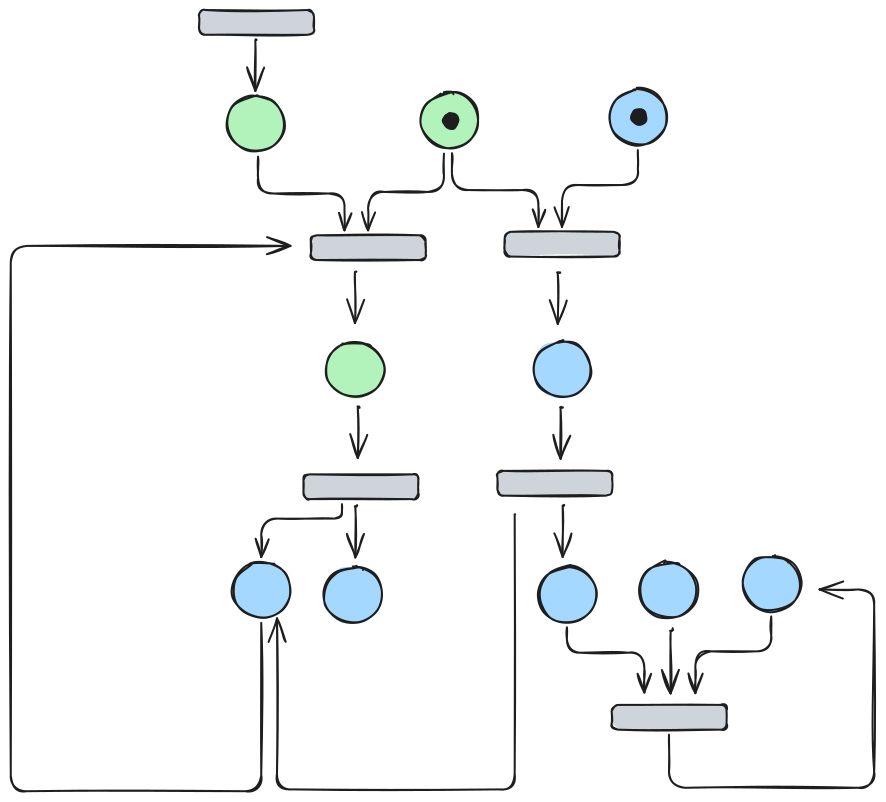
\includegraphics[width=\textwidth]{plots/bidirectional_pruning_step_a_updated.pdf}
%		\caption{Step 0: initial Petri net, before slicing.}
%		\label{fig:step:a}
%	\end{subfigure}\hfill
%	\begin{subfigure}[b]{0.45\textwidth}
%		\centering
%		\includegraphics[width=\textwidth]{plots/bidirectional_pruning_step_b_updated.pdf}
%		\caption{Step 1: first forward pass.}
%		\label{fig:step:b}
%	\end{subfigure}
%	
%	\vspace{1em}
%	
%	% Bottom row: (c), (d), and (e) matching (d)’s height
%	\begin{subfigure}[b]{0.30\textwidth}
%		\centering
%		\includegraphics[width=\textwidth]{plots/bidirectional_pruning_step_c_updated.pdf}
%		\caption{Step 2: first backward pass.}
%		\label{fig:step:c}
%	\end{subfigure}\hfill
%	\begin{subfigure}[b]{0.23\textwidth}
%		\centering
%		\includegraphics[width=\textwidth]{plots/bidirectional_pruning_step_d_updated_2.pdf}
%		\caption{Step 3: second forward pass.}
%		\label{fig:step:d}
%	\end{subfigure}\hfill
%	% <-- three-arg form: [vpos][total height][inner vpos]
%	\begin{subfigure}[b][\subfigheight][b]{0.23\textwidth}
%		\centering
%		\includegraphics[width=\textwidth]{plots/bidirectional_pruning_step_e_updated_2.pdf}
%		\caption{Step 4: final Petri net.}
%		\label{fig:step:e}
%	\end{subfigure}
%	
%	\caption{A Petri net during three rounds of bidirectional slicing: two forward passes and one backward pass. Black dots represent initial token markings; green places represent places that are allowed to be reachable in our constraints (i.e., aren't fixed to zero tokens in the final marking). Dashed shapes represent places and transitions that are identified as removable in the current iteration, and will be removed after it ends.}
%	\label{fig:bidirectional_pruning}
%\end{figure}

%\newpage

	\clearpage

\section{Evaluation: Full Results}
\label{appendix:full_results}

See Table~\ref{tab:benchmarks-all}.
%\begin{table}[htbp]
%	\centering
%	% Load the tabular from the external file:
%	\begin{table}[H]
	\centering
	\begin{tabular}{l r r r r}
		\toprule
		& \multicolumn{2}{c}{Average time (ms)} 
		& \multicolumn{2}{c}{Median time (ms)} \\
		\cmidrule(lr){2-3} \cmidrule(lr){4-5}
		Category
		& \shortstack{certificate\\generation}
		& total
		& \shortstack{certificate\\generation}
		& total \\
		\midrule
		Serializable      &   2{,}273 &  25{,}531 &  1{,}178 &  2{,}238 \\
		Not serializable  &  42{,}076 &  42{,}980 &   773 &   830 \\
		All               &  39{,}613 &  52{,}858 &   797 &  2{,}080 \\
		\bottomrule
	\end{tabular}
\end{table}

%	\caption{Average and median runtime. Values are rounded to the nearest integer, to reduce clutter. The \textit{total} column also includes the time for validation.}
%	\label{tab:stats-summary}
%\end{table}


\todo{check table}
\begin{table}[h]
	\centering
	\small
	\setlength{\tabcolsep}{5pt}
	\renewcommand{\arraystretch}{0.9}
	
	\begin{tabular*}{\textwidth}{@{\extracolsep{\fill}}%
			p{1.5cm}   % Category
			p{1.0cm}   % Benchmark
			c          % Serializable
			c c c c c c % Features
			r r        % Cert, Total
		}
		\toprule
		\multicolumn{2}{c}{\textbf{Benchmark}}
		& \textbf{Serializable}
		& \multicolumn{6}{c}{\textbf{Features}}
		& \multicolumn{2}{c}{\textbf{Runtime (ms)}} \\
		\cmidrule(lr){1-2} \cmidrule(lr){3-3} \cmidrule(lr){4-9} \cmidrule(lr){10-11}
		&
		&
		& If & While & \texttt{?} & Arith & Yield & Multi-req
		& Cert. & Total \\
		\midrule
		
		% Core expressions
		\multirow{7}{=}{Core expressions} 
		& \texttt{a1.ser} & \greencmark &  & \cmark &  &  &       &   & 2 & 47 \\
		& \texttt{a2.ser} & \xmark &  &        &  &  & \cmark &   & 280 & 296 \\
		& \texttt{a3.ser} & \greencmark &  &        &  &  &       &   & 1 & 32 \\
		& \texttt{a4.ser} & \greencmark &  &        &  &  & \cmark & \cmark & 637 & 1{,}071 \\
		& \texttt{a5.ser} & \greencmark &  & \cmark &  &  & \cmark & \cmark & 3{,}234 & 13{,}624 \\
		& \texttt{a6.ser} & \xmark &  &        &  &  & \cmark & \cmark & 757 & 775 \\
		& \texttt{a7.ser} & \greencmark & \cmark & \cmark &  &  & \cmark &   & 4 & 33 \\
		\midrule
		
		% State machines
		\multirow{4}{=}{State machines} 
		& \texttt{b1.json} & \greencmark & \cmark &        &  &  & \cmark & \cmark & 683 & 968 \\
		& \texttt{b2.json} & \greencmark & \cmark &        &  &  & \cmark & \cmark & 2{,}063 & 7{,}802 \\
		& \texttt{b3.json} & \greencmark & \cmark &        &  &  & \cmark & \cmark & 730 & 2{,}080 \\
		& \texttt{b4.json} & \greencmark & \cmark &        &  &  & \cmark & \cmark & 660 & 1{,}909 \\
		\midrule
		
		% Mixed arithmetic
		\multirow{8}{=}{Mixed arithmetic} 
		& \texttt{c1.ser} & \xmark &  & \cmark &  & \cmark & \cmark & \cmark & 356{,}195 & 356{,}299 \\
		& \texttt{c2.ser} & \greencmark &  & \cmark &  & \cmark & \cmark & \cmark & 9{,}858 & 292{,}228 \\
		& \texttt{c3.ser} & \greencmark &  & \cmark &  & \cmark & \cmark & \cmark & 1{,}886 & 2{,}397 \\
		& \texttt{c4.ser} & \greencmark &  & \cmark &  & \cmark & \cmark & \cmark & 4{,}336 & 7{,}193 \\
		& \texttt{c5.ser} & \xmark &  & \cmark &  & \cmark & \cmark & \cmark & 43{,}694 & 43{,}735 \\
		& \texttt{c6.ser} & \xmark &  & \cmark &  & \cmark & \cmark & \cmark & 629 & 698 \\
		& \texttt{c7.ser} & \xmark &  & \cmark &  & \cmark & \cmark & \cmark & 797 & 875 \\
		& \texttt{c8.ser} & \greencmark &  & \cmark &  & \cmark & \cmark & \cmark & 4{,}357 & 8{,}931 \\
		\midrule
		
		% Circular increment
		\multirow{5}{=}{Circular increment} 
		& \texttt{d1.ser} & \greencmark & \cmark & \cmark & \cmark &  & \cmark &   & 2{,}391 & 5{,}373 \\
		& \texttt{d2.ser} & \xmark & \cmark &        & \cmark &  &   \cmark &   & 628 & 731 \\
		& \texttt{d3.ser} & \greencmark & \cmark & \cmark & \cmark &  &  \cmark &   & 2{,}642 & 10{,}266 \\
		& \texttt{d4.ser} & \greencmark & \cmark & \cmark & \cmark &  &     \cmark &   & 5{,}604 & 22{,}249 \\
		& \texttt{d5.ser} & \xmark & \cmark &        &  &  & \cmark &   & 495 & 554 \\
		\midrule
		
		% Concurrency & locking loops
		\multirow{7}{=}{Concurrency \& locking loops} 
		& \texttt{e1.ser} & \greencmark &  & \cmark &  &  & \cmark &   & 351 & 502 \\
		& \texttt{e2.ser} & \xmark & \cmark & \cmark &  & \cmark & \cmark & \cmark & \texttt{TIMEOUT} & \texttt{TIMEOUT} \\
		& \texttt{e3.ser} & \xmark & \cmark & \cmark &  & \cmark &   \cmark & \cmark & 24{,}899 & 25{,}039 \\
		& \texttt{e4.ser} & \xmark & \cmark & \cmark &  &  \cmark &   \cmark & \cmark & 273{,}062 & 273{,}351 \\
		& \texttt{e5.ser} & \greencmark & \cmark & \cmark & \cmark &  & \cmark &   & 2 & 55 \\
		& \texttt{e6.ser} & \greencmark & \cmark & \cmark & \cmark &  & \cmark &   & 10 & 114 \\
		& \texttt{e7.ser} & \greencmark &  & \cmark &  &  &   \cmark &   & 299 & 444 \\
		\midrule
		
		% Non-determinism
		\multirow{9}{=}{Non-determinism} 
		& \texttt{f1.ser} & \greencmark & \cmark &    \cmark    & \cmark &  & \cmark &   & 388 & 494 \\
		& \texttt{f2.ser} & \xmark & \cmark &   \cmark     & \cmark &  & \cmark &   & 612 & 676 \\
		& \texttt{f3.ser} & \xmark &  &        &  & \cmark &   \cmark & \cmark & 653 & 716 \\
		& \texttt{f4.ser} & \greencmark &  &     \cmark   &  & \cmark & \cmark & \cmark & 1{,}626 & 9{,}515 \\
		& \texttt{f5.ser} & \greencmark & \cmark &        & \cmark &  &       &   & 7{,}401 & 11{,}301 \\
		& \texttt{f6.ser} & \xmark & \cmark &        & \cmark &  & \cmark &   & 646 & 830 \\
		& \texttt{f7.ser} & \xmark & \cmark &        & \cmark &  &  \cmark &   & 400 & 427 \\
		& \texttt{f8.ser} & \xmark & \cmark &        & \cmark &  &   \cmark &   & 773 & 802 \\
		& \texttt{f9.ser} & \greencmark & \cmark &        & \cmark &  &  \cmark &   & 10 & 94 \\
		\midrule
		
		% Network & system protocols
		\multirow{7}{=}{Network \& system protocols} 
		& \texttt{g1.ser} & \xmark & \cmark & \cmark &  & \cmark & \cmark & \cmark & 59{,}312 & 74{,}539 \\
		& \texttt{g2.ser} & \greencmark & \cmark & \cmark &  & \cmark & \cmark & \cmark & \texttt{TIMEOUT} & \texttt{TIMEOUT} \\
		& \texttt{g3.ser} & \xmark & \cmark & \cmark & \cmark & \cmark & \cmark & \cmark & 20{,}557 & 20{,}954 \\
		& \texttt{g4.ser} & \xmark & \cmark & \cmark & \cmark & \cmark & \cmark & \cmark & 6{,}859 & 7{,}047 \\
		& \texttt{g5.ser} & \greencmark & \cmark & \cmark & \cmark & \cmark &   \cmark & \cmark & 3{,}047 & 12{,}324 \\
		& \texttt{g6.ser} & \xmark & \cmark &        & \cmark & \cmark & \cmark &   & 8{,}193 & 8{,}285 \\
		& \texttt{g7.ser} & \greencmark & \cmark &        & \cmark & \cmark &       &   & 6{,}886 & 252{,}752 \\
		\bottomrule
	\end{tabular*}
	
	\caption{Overview of our benchmarks and semilinear set reductions (timeouts: 500 ms).}
	\label{tab:benchmarks-all}
\end{table}



%\begin{table}[htbp]
%	\centering
%	% Load the tabular from the external file:
%	\begin{table}[H]
	\centering
	\small
	% increase horizontal padding between columns
	\setlength{\tabcolsep}{5pt}
	\renewcommand{\arraystretch}{0.9}
	\begin{tabular*}{\textwidth}{@{\extracolsep{\fill}}%
			p{1.5cm}   % Category
			p{1.0cm} % Benchmark
			c        % Serializable
			c c c c c c % Features
			r r       % Cert, Total
		}
		\toprule
		\multicolumn{2}{c}{\textbf{Benchmark}}
		& \textbf{Serializable}
		& \multicolumn{6}{c}{\textbf{Features}}
		& \multicolumn{2}{c}{\textbf{Runtime (ms)}} \\
		\cmidrule(lr){1-2} \cmidrule(lr){3-3} \cmidrule(lr){4-9} \cmidrule(lr){10-11}
		&
		&
		& If & While & \texttt{?} & Arith & Yield & Multi-req
		& Cert. & Total \\
		\midrule
		\multirow{7}{=}{Core expressions} & \texttt{a1.ser} & \greencmark &  & \cmark &  &  &       &   & 2 & 47 \\
		 & \texttt{a2.ser} & \xmark &  &        &  &  & \cmark &   & 280 & 296 \\
		 & \texttt{a3.ser} & \greencmark &  &        &  &  &       &   & 1 & 32 \\
		 & \texttt{a4.ser} & \greencmark &  &        &  &  & \cmark & \cmark & 637 & 1{,}071 \\
		 & \texttt{a5.ser} & \greencmark &  & \cmark &  &  & \cmark & \cmark & 3{,}234 & 13{,}624 \\
		 & \texttt{a6.ser} & \xmark &  &        &  &  & \cmark & \cmark & 757 & 775 \\
		 & \texttt{a7.ser} & \greencmark & \cmark & \cmark &  &  & \cmark &   & 4 & 33 \\
		\midrule
		\multirow{4}{=}{State machines} & \texttt{b1.json} & \greencmark & \cmark &        &  &  & \cmark & \cmark & 683 & 968 \\
		 & \texttt{b2.json} & \greencmark & \cmark &        &  &  & \cmark & \cmark & 2{,}063 & 7{,}802 \\
		 & \texttt{b3.json} & \greencmark & \cmark &        &  &  & \cmark & \cmark & 730 & 2{,}080 \\
		 & \texttt{b4.json} & \greencmark & \cmark &        &  &  & \cmark & \cmark & 660 & 1{,}909 \\
		\midrule
		\multirow{8}{=}{Mixed arithmetic} & \texttt{c1.ser} & \xmark &  & \cmark &  & \cmark & \cmark & \cmark & 356{,}195 & 356{,}299 \\
		 & \texttt{c2.ser} & \greencmark &  & \cmark &  & \cmark & \cmark & \cmark & 9{,}858 & 292{,}228 \\
		 & \texttt{c3.ser} & \greencmark &  & \cmark &  & \cmark & \cmark & \cmark & 1{,}886 & 2{,}397 \\
		 & \texttt{c4.ser} & \greencmark &  & \cmark &  & \cmark & \cmark & \cmark & 4{,}336 & 7{,}193 \\
		 & \texttt{c5.ser} & \xmark &  & \cmark &  & \cmark & \cmark & \cmark & 43{,}694 & 43{,}735 \\
		 & \texttt{c6.ser} & \xmark &  & \cmark &  & \cmark & \cmark & \cmark & 629 & 698 \\
		 & \texttt{c7.ser} & \xmark &  & \cmark &  & \cmark & \cmark & \cmark & 797 & 875 \\
		 & \texttt{c8.ser} & \greencmark &  & \cmark &  & \cmark & \cmark & \cmark & 4{,}357 & 8{,}931 \\
		\midrule
		\multirow{5}{=}{Circular increment} & \texttt{d1.ser} & \greencmark & \cmark & \cmark & \cmark &  & \cmark &   & 2{,}391 & 5{,}373 \\
		 & \texttt{d2.ser} & \xmark & \cmark &        & \cmark &  &   \cmark &   & 628 & 731 \\
		 & \texttt{d3.ser} & \greencmark & \cmark & \cmark & \cmark &  &  \cmark &   & 2{,}642 & 10{,}266 \\
		 & \texttt{d4.ser} & \greencmark & \cmark & \cmark & \cmark &  &     \cmark &   & 5{,}604 & 22{,}249 \\
		 & \texttt{d5.ser} & \xmark & \cmark &        &  &  & \cmark &   & 495 & 554 \\
		\midrule
		\multirow{7}{=}{Concurrency \& locking loops} & \texttt{e1.ser} & \greencmark &  & \cmark &  &  & \cmark &   & 351 & 502 \\
		 & \texttt{e2.ser} & \xmark & \cmark & \cmark &  & \cmark & \cmark & \cmark & \texttt{TIMEOUT} & \texttt{TIMEOUT} \\
		 & \texttt{e3.ser} & \xmark & \cmark & \cmark &  & \cmark &   \cmark & \cmark & 24{,}899 & 25{,}039 \\
		 & \texttt{e4.ser} & \xmark & \cmark & \cmark &  &  \cmark &   \cmark & \cmark & 273{,}062 & 273{,}351 \\
		 & \texttt{e5.ser} & \greencmark & \cmark & \cmark & \cmark &  & \cmark &   & 2 & 55 \\
		 & \texttt{e6.ser} & \greencmark & \cmark & \cmark & \cmark &  & \cmark &   & 10 & 114 \\
		 & \texttt{e7.ser} & \greencmark &  & \cmark &  &  &   \cmark &   & 299 & 444 \\
		\midrule
		\multirow{9}{=}{Non-deterministic \& randomness} & \texttt{f1.ser} & \greencmark & \cmark &    \cmark    & \cmark &  & \cmark &   & 388 & 494 \\
		 & \texttt{f2.ser} & \xmark & \cmark &   \cmark     & \cmark &  & \cmark &   & 612 & 676 \\
		 & \texttt{f3.ser} & \xmark &  &        &  & \cmark &   \cmark & \cmark & 653 & 716 \\
		 & \texttt{f4.ser} & \greencmark &  &     \cmark   &  & \cmark & \cmark & \cmark & 1{,}626 & 9{,}515 \\
		 & \texttt{f5.ser} & \greencmark & \cmark &        & \cmark &  &       &   & 7{,}401 & 11{,}301 \\
		 & \texttt{f6.ser} & \xmark & \cmark &        & \cmark &  & \cmark &   & 646 & 830 \\
		 & \texttt{f7.ser} & \xmark & \cmark &        & \cmark &  &  \cmark &   & 400 & 427 \\
		 & \texttt{f8.ser} & \xmark & \cmark &        & \cmark &  &   \cmark &   & 773 & 802 \\
		 & \texttt{f9.ser} & \greencmark & \cmark &        & \cmark &  &  \cmark &   & 10 & 94 \\
		\midrule
		\multirow{7}{=}{Networking \& system protocols} & \texttt{g1.ser} & \xmark & \cmark & \cmark &  & \cmark & \cmark & \cmark & 59{,}312 & 74{,}539 \\
		 & \texttt{g2.ser} & \greencmark & \cmark & \cmark &  & \cmark & \cmark & \cmark & \texttt{TIMEOUT} & \texttt{TIMEOUT} \\
		 & \texttt{g3.ser} & \xmark & \cmark & \cmark & \cmark & \cmark & \cmark & \cmark & 20{,}557 & 20{,}954 \\
		 & \texttt{g4.ser} & \xmark & \cmark & \cmark & \cmark & \cmark & \cmark & \cmark & 6{,}859 & 7{,}047 \\
		 & \texttt{g5.ser} & \greencmark & \cmark & \cmark & \cmark & \cmark &   \cmark & \cmark & 3{,}047 & 12{,}324 \\
		 & \texttt{g6.ser} & \xmark & \cmark &        & \cmark & \cmark & \cmark &   & 8{,}193 & 8{,}285 \\
		 & \texttt{g7.ser} & \greencmark & \cmark &        & \cmark & \cmark &       &   & 6{,}886 & 252{,}752 \\
		\midrule
\bottomrule
	\end{tabular*}
\end{table}

%	\caption{Overview of our benchmarks (\texttt{TIMEOUT} is $500$ seconds).}
%	\label{tab:benchmarks-all}
%\end{table}





\subsection{Optimization Analysis}
\label{subsec:optimization-results}

%Next of our four optimizations, and analyzed their effect on the overall runtime and space resources.
%
%All experiments were run with a \texttt{TIMEOUT} value of $150$ seconds.


\subsubsection{Runtime optimization.}

We ran all benchmarks with each of the following six optimization configurations: 
(i) without any optimization (marked [\texttt{\textbf{\text{-}\text{-}\text{-}\text{-}}}] in Fig.~\ref{fig:timeout_cumulative_solved_log}); (ii) with bidirectional slicing (marked [\texttt{\textbf{\text{B}\text{-}\text{-}\text{-}}}]); (iii) with redundant constraint elimination (marked [\texttt{\textbf{\text{-}\text{R}\text{-}\text{-}}}]); (iv) with generation of fewer constraints (marked [\texttt{\textbf{\text{-}\text{-}\text{G}\text{-}}}]);
(v) with strategic Kleene elimination (marked [\texttt{\textbf{\text{-}\text{-}\text{-}\text{S}}}]);
and finally, (vi) with all optimizations altogether (marked [\texttt{\textbf{\text{B}\text{R}\text{G}\text{S}}}]).
%
The results of the aggregated runtimes are presented in Fig.~\ref{fig:timeout_cumulative_solved_log} and show that over $28\%$ more benchmarks are solved when using all optimizations compared to running without any optimization.
%
Not surprisingly, the best configuration is the one with all optimizations on. 
%
Furthermore, the best single-optimization configurations with regard to runtime are [\texttt{\textbf{\text{-}\text{-}\text{G}\text{-}}}] and [\texttt{\textbf{\text{B}\text{-}\text{-}\text{-}}}], solving over $74\%$ and $72\%$ of the benchmarks respectively. 
%
We also note that the two remaining optimizations, [\texttt{\textbf{\text{-}\text{R}\text{-}\text{-}}}] and [\texttt{\textbf{\text{-}\text{-}\text{-}\text{S}}}], performed slightly worse (although not significantly) than without the optimizations when counting overall timeouts.
%
However, when analyzing the redundant constraint optimization (  [\texttt{\textbf{\text{-}\text{R}\text{-}\text{-}}}]), we identified instances in which it still \textit{strictly} improves runtime.
%
For example, the optimization affords a speedup of between $72.2\%$ and $85.2\%$ for benchmarks \texttt{a3.ser} and \texttt{a7.ser},  when compared to the baseline.

\subsubsection{Space optimization.}
Our optimizations also reduce the space complexity of the two main components --- the Petri net and the semilinear set.

\noindent
(1) \textbf{Petri net.} Bidirectional slicing (Fig.~\ref{fig:petri_size_reduction}) 
eliminates the average number of places \textit{by roughly half} --- from $23.91$ down to $12.79$. This optimization proved even more effective on transitions, \textit{eliminating about two-thirds}: from $37.3$ down to $12.61$. 
%Note that the pre-pruning averages were computed over $47$ nets (one per benchmark), whereas the post-pruning averages span $224$ nets, since each pre-pruning net gives rise to a separate pruned net per each disjunct.  
%\\

\noindent
(2) \textbf{Semilinear sets.} We ran an ablation experiment in which we compared all optimizations against runs where each of the three semilinear optimizations (i.e., all but PN slicing) was disabled. The redundant-constraint elimination (with a negated effect in [\texttt{\textbf{\text{B}\textcolor{red}{-}\text{G}\text{S}}}]) and the fewer-constraint generation elimination (with a negated effect in [\texttt{\textbf{\text{B}\text{R}\textcolor{red}{-}\text{S}}}]) \textit{drastically} reduced component counts, with the latter being especially effective in reducing the \textit{maximal} number of components to be up to $\mathbf{931\times}$ smaller, and the \textit{average} number of components to be up to $\mathbf{223\times}$ smaller (Table~\ref{tab:semilinear-size-reduction}), when compared to the baseline executions configured with all optimizations on ([\texttt{\textbf{\text{B}\text{R}\text{G}\text{S}}}]). 
%
For fairness, we measured only benchmarks completed under all configurations, excluding cases where semilinear sets exploded beyond $2^{30}$ components and timed out. Thus, our reported improvements actually \textit{understate} the true impact of these optimizations on memory. Such blowups, %especially common in state-machine benchmarks with NS loops, 
render even simple programs intractable without these optimizations.


%\subsubsection{Space Optimization}
%
%Our optimizations also reduce the space complexity of the two main components --- the Petri Net and the semilinear set.
%
%\smallskip
%\noindent
%\textbf{Petri Net size reduction.}
%%
%With all optimizations enabled, we evaluated (Fig.~\ref{fig:petri_size_reduction}) the impact of our bidirectional pruning by comparing, across all benchmarks, the average number of places and transitions removed due to this optimization. On average, pruning reduced the number of places \textit{by roughly half} --- dropping from $23.91$ places before pruning to $12.79$ places afterward. Pruning proved even more effective on transitions, \textit{eliminating about two-thirds} of them: from $37.3$ transitions on average before pruning down to $12.61$ afterward. Note that the pre-pruning averages were computed over $47$ nets (one per benchmark), whereas the post-pruning averages span $224$ nets, since each pre-pruning net gives rise to a separate pruned net per each disjunct. 
%of our reachability query. 
%These results are summarized in Fig.~\ref{fig:petri_size_reduction}.

%When running our tool with all optimizations on, we analyzed the effect of our bidirectional pruning, This was done be counting the average number of places and transitions before and after pruning, on all benchmarks.
%%
%The pruning resulted in a reduction of about half the number of original places --- from $23.91$ places on average \textit{before} pruning to $12.79$ places on average \textit{after} pruning.
%%
%The bidirectional was even more effective in reducing the transitions, as demonstrated by a removing about two thirds of the transitions --- resulting in pruned Petri Nets with $37.30$ transitions on average \textit{before} pruning to $12.61$ transitions on average \textit{after} pruning.
%%
%We note that the averaging for the pre-pruning step was done on $47$ nets, once per each benchmark, while the averaging for the post-pruning step was done on $224$ nets, as each pre-pruning net can give rise to multiple post-pruning nets, one per each disjunct in our reachability query.
%%
%These results are presented in Fig.~\ref{fig:petri_size_reduction}.


%Number of values for 'Before' bars:          47
%Number of values for 'After' bars:           224
%Average number of places before pruning:     23.91
%Average number of places after pruning:      12.79
%Average number of transitions before pruning: 37.30
%Average number of transitions after pruning:  12.61






%\smallskip
%\noindent
%\textbf{Semilinear set size reduction.}
%%
%Finally, our last experiment batch analyzed the size reduction among the semilinear sets.
%%
%Towards this end, we ran all our benchmarks with all optimizations to serve as a baseline. 
%%
%Then, we analyzed the effect of the three semilinear-related optimizations, i.e., all but the bidirectional pruning. For each of these three optimizations, we ran the benchmarks with all optimizations \textit{except} the one checked.
%%
%%Table~\ref{tab:semilinear-size-reduction} include a summary of the results, when comparing the semilinear set size.
%%
%Specifically, we compare both the average and the maximal (i) number of components; and (ii) period vectors per each component, as summarized in Table~\ref{tab:semilinear-size-reduction}.
%%
%The redundant constraint elimination and the generate-less-constraints optimizations had a highly significant effect on the number of components, with the latter being especially effective in reducing the maximal number of components to be $931$ times more compact, as well as the average number of components to be $223$ times more compact, when compared to the baseline.
%%
%To ensure a fair comparison, we only measured benchmarks that were completed under every configuration, deliberately excluding any case where the optimized semilinear set exploded beyond $2^{30}$ components and timed out. By excluding these intractable runs, our reported performance improvements actually \textit{understate} the true impact of these optimizations. This explosive growth and the resulting timeouts are especially pervasive among our state-machine benchmarks due to loops in their NS, rendering even simple programs infeasible without optimizations.
%
%In fact, for both these optimizations are even more effective as, in order to conduct a fair comparison, we analyzed only benchmarks that terminated in all combinations, an hence we do not include cases in which these two optimizations rendered the original semilinear set intractable, due to having over $2^{30}$ components (!), hence timing-out and being excluded from the analysis.
%%
%This occurs pervasively in our state-machine benchmarks which have loops in their network systems --- and hence even simple programs of this category cannot be analyzed with respect to serializability.

%\todo{understand why this is related to loops in the NS}

%
%\begin{center}
%	\begin{minipage}[htbp]{0.48\textwidth}
%		\centering
%		\includegraphics[width=\linewidth]{figures/cactus_plot.pdf}
%		\captionof{figure}{Solved instances (\texttt{TIMEOUT} $150$ s).}
%		\label{fig:timeout_cumulative_solved_log}
%	\end{minipage}\hfill
%	\begin{minipage}[htbp]{0.48\textwidth}
%		\centering
%		\includegraphics[width=\linewidth]{figures/petri_size_reduction_plot.pdf}
%		\captionof{figure}{PN size reduction via slicing.}
%		%(timeout 150 seconds)
%		%.}
%	\label{fig:petri_size_reduction}
%\end{minipage}
%\end{center}

%


\begin{figure}[h]
	\centering
	\includegraphics[width=0.68\linewidth]{figures/cactus_plot.pdf}
	\caption{Solved instances (\texttt{TIMEOUT} is 150 seconds).}
	\label{fig:timeout_cumulative_solved_log}
\end{figure}

%\begin{table}[!htbp]
%	\centering
%		\includegraphics[width=0.68\linewidth]{figures/cactus_plot.pdf}
%	\captionof{figure}{Solved instances (\texttt{TIMEOUT} is $150$ seconds).}
%	\label{fig:timeout_cumulative_solved_log}
%\end{table}


\begin{figure}[h]
	\centering
	\includegraphics[width=0.68\linewidth]{figures/petri_size_reduction_plot.pdf}
	\caption{PN size reduction via slicing.}
	\label{fig:petri_size_reduction}
\end{figure}



%\begin{table}[!htbp]
%	\centering
%	\includegraphics[width=0.68\linewidth]{figures/petri_size_reduction_plot.pdf}
%	\captionof{figure}{PN size reduction via slicing.}
%	%(timeout 150 seconds)
%	%.}
%	\label{fig:petri_size_reduction}
%\end{table}

%\begin{table}[!htbp]
%\centering
%\begin{minipage}[t]{0.48\linewidth}
%	\centering
%	\begin{table}[H]
	\centering
	\begin{tabular}{l r r r r}
		\toprule
		& \multicolumn{2}{c}{Average (ms)} 
		& \multicolumn{2}{c}{Median (ms)} \\
		\cmidrule(lr){2-3} \cmidrule(lr){4-5}
		Category
		& \shortstack{cert.}
		& total
		& \shortstack{cert.}
		& total \\
		\midrule
		\textcolor{ForestGreen}{Serializable}      &   2{,}273 &  25{,}531 &  1{,}178 &  2{,}238 \\
		\textcolor{red}{Not serializable}  &  42{,}076 &  42{,}980 &   773 &   830 \\
		All               &  39{,}613 &  52{,}858 &   797 &  2{,}080 \\
		\bottomrule
	\end{tabular}
\end{table}

%	\caption{Runtime for generated certificates (\texttt{total} also includes validation).}
%	%			Values are rounded to the nearest integer, to reduce clutter. 
%	%The \textit{total} column also includes the time for validation.}
%% NOTE - this excludes the 2 non-terminating runs (artifact also includes TIMEOUTs I think)
%\label{tab:stats-summary}
%\end{minipage}\hfill
%\begin{minipage}[t]{0.48\linewidth}
%\centering
%\begin{table}[H]
	\centering
	\begin{tabular}{l c c c c}
		\toprule
		& \multicolumn{2}{c}{components} & \multicolumn{2}{c}{periods/component} \\
		\cmidrule(lr){2-3} \cmidrule(lr){4-5}
		& average & max & average & max \\
		\midrule
	\texttt{\text{B}\text{R}\text{G}\text{S}} & 2.91 & 22 & 1.33 & 4 \\
	\texttt{\text{B}\textcolor{red}{-}\text{G}\text{S}} & 8.79 & 194 & \textbf{1.64} & 11 \\
	\texttt{\text{B}\text{R}\textcolor{red}{-}\text{S}} & \textbf{651.41} & \textbf{20{,}484} & 1.28 & \textbf{15} \\
	\texttt{\text{B}\text{R}\text{G}\textcolor{red}{-}} & 2.91 & 22 & 1.35 & 4 \\
  \bottomrule
	\end{tabular}
\end{table}

%\caption{Semilinear set size reduction via optimizations (baseline is [\texttt{\text{B}\text{R}\text{G}\text{S}}]).}
%\label{tab:semilinear-size-reduction}
%\end{minipage}
%\end{table}





%\begin{table}[!htbp]
%	\centering
%	\begin{table}[H]
	\centering
	\begin{tabular}{l c c c c}
		\toprule
		& \multicolumn{2}{c}{components} & \multicolumn{2}{c}{periods/component} \\
		\cmidrule(lr){2-3} \cmidrule(lr){4-5}
		& average & max & average & max \\
		\midrule
	\texttt{\text{B}\text{R}\text{G}\text{S}} & 2.91 & 22 & 1.33 & 4 \\
	\texttt{\text{B}\textcolor{red}{-}\text{G}\text{S}} & 8.79 & 194 & \textbf{1.64} & 11 \\
	\texttt{\text{B}\text{R}\textcolor{red}{-}\text{S}} & \textbf{651.41} & \textbf{20{,}484} & 1.28 & \textbf{15} \\
	\texttt{\text{B}\text{R}\text{G}\textcolor{red}{-}} & 2.91 & 22 & 1.35 & 4 \\
  \bottomrule
	\end{tabular}
\end{table}

%	\caption{Semilinear set size reduction via optimizations (baseline is [\texttt{\text{B}\text{R}\text{G}\text{S}}]).}
%	\label{tab:semilinear-size-reduction}
%\end{table}

\todo{check table}
%
\begin{table}[h]
	\centering
	\begin{tabular}{l c c c c}
		\toprule
		& \multicolumn{2}{c}{components} & \multicolumn{2}{c}{periods/component} \\
		\cmidrule(lr){2-3} \cmidrule(lr){4-5}
		& average & max & average & max \\
		\midrule
		\texttt{BRGS} & 2.91 & 22 & 1.33 & 4 \\
		\texttt{B}\textcolor{red}{-}\texttt{GS} & 8.79 & 194 & \textbf{1.64} & 11 \\
		\texttt{BR}\textcolor{red}{-}\texttt{S} & \textbf{651.41} & \textbf{20{,}484} & 1.28 & \textbf{15} \\
		\texttt{BRG}\textcolor{red}{-} & 2.91 & 22 & 1.35 & 4 \\
		\bottomrule
	\end{tabular}
	\caption{Semilinear set size reduction via optimizations (baseline is \texttt{BRGS}).}
	\label{tab:semilinear-size-reduction}
\end{table}


	
\end{document}